 %\documentclass[1.5headlines,twoside, a4paper, 11pt, automark,final,headsepline]{scrreprt}
\documentclass[1.5headlines,twoside, openright, a4paper, 12pt, automark,final,headsepline, hidelinks]{scrbook}

%%****************
%% define medatata
%%________________
%\def\Title{An Example Document}
%\def\Author{Some Name}
%\def\Subject{An Example Document}
%\def\Keywords{LaTeX,Example,Document}
% 
%%***************************************************************************
%% \convertDate converts D:20080419103507+02'00' to 2008-04-19T10:35:07+02:00
%%___________________________________________________________________________
%\def\convertDate{%
%    \getYear
%}
% 
%{\catcode`\D=12
% \gdef\getYear D:#1#2#3#4{\edef\xYear{#1#2#3#4}\getMonth}
%}
%\def\getMonth#1#2{\edef\xMonth{#1#2}\getDay}
%\def\getDay#1#2{\edef\xDay{#1#2}\getHour}
%\def\getHour#1#2{\edef\xHour{#1#2}\getMin}
%\def\getMin#1#2{\edef\xMin{#1#2}\getSec}
%\def\getSec#1#2{\edef\xSec{#1#2}\getTZh}
%\def\getTZh +#1#2{\edef\xTZh{#1#2}\getTZm}
%\def\getTZm '#1#2'{%
%    \edef\xTZm{#1#2}%
%    \edef\convDate{\xYear-\xMonth-\xDay T\xHour:\xMin:\xSec+\xTZh:\xTZm}%
%}
% 
%\expandafter\convertDate\pdfcreationdate 
% 
%%**************************
%% get pdftex version string
%%__________________________
%\newcount\countA
%\countA=\pdftexversion
%\advance \countA by -100
%\def\pdftexVersionStr{pdfTeX-1.\the\countA.\pdftexrevision}
% 
% 
%%*********
%% XMP data
%\usepackage{xmpincl}
%
%
%\providecommand{\xmpAuthorURI}{} \providecommand{\xmpJournalnumber}{} \providecommand{\xmpVolume}{} \providecommand{\xmpIssue}{} \providecommand{\xmpCoverDisplayDate}{} \providecommand{\xmpCoverDate}{} \providecommand{\xmpJournaltitle}{} \providecommand{\xmpFirstpage}{} \providecommand{\xmpLastpage}{} \providecommand{\xmpDoi}{}
%
%
%\providecommand{\xmpProducer}{LaTeX2e}
%\providecommand{\xmpOrg}{MyOrg}
%\providecommand{\xmpTitle}{MyTitle}
%\providecommand{\xmpAuthor}{MyAuthor, mymail@gmail.com}
%\providecommand{\xmpKeywords}{MyKeywords}
%\providecommand{\xmpSubject}{MySubject}
%\providecommand{\xmpCreatorTool}{\pdftexbanner}
%\providecommand{\convDate}{\pdfcreationdate}
%\makeatletter
%
%\includexmp{pdfa-1b}
%\makeatother
% 
%%********
%% pdfInfo
%%________
%\pdfinfo{%
%    /Title    (\Title)
%    /Author   (\Author)
%    /Subject  (\Subject)
%    /Keywords (\Keywords)
%    /ModDate  (\pdfcreationdate)
%    /Trapped  /False
%}
%%****************************************
%% include the packages, commands and glossaries
\usepackage[a-1b]{pdfx}
\usepackage{xmpincl}
\usepackage[inner=3.0cm,outer=2cm,top=2cm,bottom=2cm,includeheadfoot]{geometry}
\usepackage[onehalfspacing]{setspace}
%\setstretch{baselinestretch}
%\linespread{1.5} % line spacing 
 
\usepackage[headsepline,plainheadsepline]{scrpage2}
\let\endgraph\endgraf        % necessary for "chapterprefix" in \documentclass call

% Header and footer definition
\clearscrheadfoot            % clear header and footer
\ohead[\headmark]{\headmark} % chapter names at top
\automark[section]{chapter}
\pagestyle{scrheadings}      % choose page style
%
%% % try to solve the width problem in PDF/A
%\usepackage[T1]{fontenc}

\ofoot[\pagemark]{\pagemark} % page number on the upper right side
%--------- separate abstract and content with one blank page---------- %
\usepackage{afterpage}
\newcommand\blankpage{%
    \null
    \thispagestyle{empty}%
    \addtocounter{page}{-1}%
    \newpage}
%\usepackage[backend=biber]{biblatex}
% ------ Language and Text Options
\usepackage[english]{babel}
\usepackage[latin9]{inputenc}
%\usepackage{pdflatex}
%\usepackage{color}
\usepackage{float}
%\usepackage{xmpincl}
\usepackage{hyperref}

%******** complexity O()*******
\usepackage{flushend}
\renewcommand{\O}[1]{$\mathcal{O}(#1)$}


%*********inline list
\usepackage{enumerate}
\usepackage[inline,shortlabels]{enumitem}

%%********inkscape to latex*************
%\usepackage{pstricks}
%%\usepackage{pst-plot}

%\usepackage[pdftex,
%        pdftoolbar=true, hyperfootnotes=false,breaklinks=true,
%        pdfpagelabels=true,
%        bookmarks, bookmarksopen, bookmarksnumbered, bookmarksopenlevel=1,
%        pdfauthor={Yanqiu Huang},
%        pdfsubject={Dissertation},%
%        pdfkeywords={WSNs, Energy efficiency, Data compression},
%        pdftitle={Dissertation,Yanqiu Huang,Uni-Bremen,2017},
%        pdfstartview={FitH},
%        pdfborder={0 0 0},  %Farbe aller Linkumrandung auf Wei� gesetzt
%        plainpages=false]{hyperref}
%\def\UrlBreaks{\do\/\do-}

% this package is used to remove the double printed math symbole problem
\usepackage{newtxtext,newtxmath}

\usepackage{etoc}
% ------ Math Packages
\usepackage{amsfonts}
\usepackage{amsmath}
\usepackage{bm}
%\usepackage{amssymb}
\newcommand\numberthis{\addtocounter{equation}{1}\tag{\theequation}}
%\usepackage{mathtools}
\usepackage[detect-none]{siunitx}
\usepackage[capitalize]{cleveref}
% ------ Source Code
\usepackage{listings}
%\usepackage{enumerate}
% ----- Floating Opjects
\usepackage{graphicx}
\usepackage{subfig}
\usepackage{xcolor}

%***packages for inputing the tikz pictures**********
\newlength\figureheight 
\newlength\figurewidth

\usepackage{pgfplots}
%******** change the tick, label size of the tikz figures********
\pgfplotsset{every axis/.append style={
		label style={font=\small},
		tick label style={font=\small}  
	}}
	
\usepackage{units}	
\usepackage{color}
	
\usepackage{epstopdf}
\usepackage{rotating}
\usepackage{multirow}		% -- multirow and multicolumn
\usepackage{booktabs}		% -- professional tables in LaTeX ,
\usepackage{longtable}
\usepackage{capt-of}
%\usepackage[bf]{caption}		% -- customise Captions
\usepackage{caption}		% -- customise Captions
\usepackage{placeins} 		% -- FloatBarrier
\usepackage{xspace}			% -- for a better layout of spaces


% ------ Table of Contents
\usepackage{minitoc}
%\dominitoc % for minitoc, default left-bounded
\setcounter{tocdepth}{4}
\setcounter{secnumdepth}{2}

% Packages for acronyms and list of symbols
%\usepackage{acronym}
\usepackage{makeidx}
\usepackage[section,style=alttree, sort=use]{glossaries}
\glssetwidest{ADCADCA}% widest name
\renewcommand*{\glsnamefont}[1]{\textmd{#1}}
\GlsSetQuote{+}
\usepackage{ifthen}

% *** SPECIALIZED LIST PACKAGES ***
\usepackage[flushleft]{threeparttable}
\usepackage[ruled, vlined, linesnumbered]{algorithm2e}
%\usepackage{algpseudocode}
%\usepackage[ruled,vlined,linesnumbered]{algorithm2e}
\usepackage{algorithmic}
\newtheorem{theorem}{Theorem}
\newenvironment{proof}[1][Proof]{\begin{trivlist}
\item[\hskip \labelsep {\bfseries #1}]}{\end{trivlist}}
%------ package for list of symbols
%\usepackage{glossaries}
\usepackage[]{appendix}		% -- include packages
% -- define your own commands
\newcommand\Fig[1]{\textbf{Fig.}~\ref{#1}}
\newcommand\fig[1]{\textbf{Fig.}~\ref{#1}}
\newcommand\Tab[1]{\textbf{Tab.}~\ref{#1}}
\newcommand\tab[1]{\textbf{Tab.}~\ref{#1}}
\newcommand\Equ[1]{\textbf{Eq.}~(\ref{#1})}
\newcommand\equ[1]{\textbf{Eq.}~(\ref{#1})}
\newcommand\Sect[1]{\textbf{Sec.}~\ref{#1}}
\newcommand\sect[1]{\textbf{Sec.}~\ref{#1}}
\newcommand\Refs[1]{\textbf{Ref.}~\cite{#1}}
\newcommand\refs[1]{\textbf{Ref.}~\cite{#1}}
\newcommand\Algo[1]{\textbf{Algorithm}~\ref{#1}}
\newcommand\algo[1]{\textbf{Algorithm}~\ref{#1}}
		% -- define your own commands
 %\clearpage
%\chapter{List of glossaries}
%\makeglossaries
%\makenoidxglossaries
%\printglossary
%\printnoidxglossary
%\newglossary*{acronym}{Acronym}
%\newglossary{acronym}{1i}{1o}{Acronym}
%\newacronym{wsn}{WSN}{wireless sensor network}
%\newacronym{pdf}{PDF}{probability density function}
\newacronym{cdf}{CDF}{Cumulative Density Function}
%\newacronym{mvn}{MVN}{multivariate normal}
%\newacronym{ridp}{Rand-idp}{Reconstruction solution using spatial and temporal correlation under random transmission}
\newcommand{\Axor}{A_\textnormal{{xor}}} % Size of a xor in math mode
\newcommand{\Aand}{A_\textnormal{{and}}} % Size of an and in math mode
\newcommand{\Amux}{A_\textnormal{{mux}}} % Size of an xor in math mode
\newcommand{\Aff}{A_\textnormal{{ff}}} % Size of an xor in math mode
\newcommand{\Txor}{T_\textnormal{{xor}}} % Size of a xor in math mode
\newcommand{\Tand}{T_\textnormal{{and}}} % Size of an and in math mode
\newcommand{\Tmux}{T_\textnormal{{mux}}} % Size of an xor in math mode
\newcommand{\ldceil}[1]{\lceil\log_2{\left({#1}\right)}\rceil}
\newcommand{\T}{{{S}}}
\newcommand{\cf}{{\delta}}
\newcommand{\PerM}{\mathbf{I}_\pi} % Definition of the Permutation matrix (I because der of Identity matrix)
\newcommand{\AssM}{\mathbf{I}_\sigma} % Definition of the assignment matrix (aus dem deutschen wikipedia "vozeichenbehaftete permutatiosnmatrix)
\newcommand{\AssOpt}{\mathbf{{I}_{\sigma,\textnormal{power-opt}}}} % Power-optimal assignment
\newcommand{\PerMCacOpt}{\mathbf{I}_{\pi,\textnormal{perf-opt}}}  % perf/CAC-opt assignment
\newcommand{\PerMTCOpt}{\mathbf{I}_{\pi,\textnormal{$\mathit{TC}$-opt}}} %Power+Perf.-opt assignment

% mean probability entry for the capacitance model
\newcommand{\meanP}{\bar{p}}

%----------------symbols------------------- %
\newglossary{math}{2i}{2o}{General mathematical symbols and specific operators}

%% \newglossaryentry{gf2}
%% { type=math, 
%%   name={\ensuremath{\mathbb{F}_2}},
%%   description={binary Galois field 2},
%%   %sort={F_2}
%% }

\newglossaryentry{log2}
{ type=math, 
	name={\ensuremath{\log_2(x)}},
	description={binary (base 2) logarithm of $x$},
	sort={log_2}
}




\newglossaryentry{bn}
{ type=math, 
	name={\ensuremath{\mathbb{N}}},
	description={set of  natural numbers: \{0,1,2,3,\dots \}},
	%sort={N}
}



%% \newglossaryentry{bb}
%% { type=math,
%%   name={\ensuremath{\mathbb{B}}},
%%   description={set of  binary numbers: \{0,1\}},
%%   %sort={B}
%% }

%% \newglossaryentry{bb_vec}
%% { type=math,
%%   name={\ensuremath{\mathbb{B}^n}},
%%   description={vector of $n$   binary numbers},
%%   %sort={B_n}
%% }

%% \newglossaryentry{bnm}
%% { type=math,
%%   name={\ensuremath{\mathbb{B}^{n\times m}}},
%%   description={matrix with $n$ rows and $m$ columns of binary numbers},
%%   %sort={B_nm}
%% }

%% \newglossaryentry{must_satisfy}
%% { type=math,
%%   name={\ensuremath{\stackrel{{ !}}{=}}},
%%   description={demanded equality},
%%   %sort={OPERATOR: demanded equality}
%% }



%% \newglossaryentry{defined}
%% { type=math,
%%   name={\ensuremath{\stackrel{{\textnormal{def}}}{=} }},
%%   description={defined as being equal to},
%%   %sort={OPERATOR: defined as being equal to}
%% }


%% \newglossaryentry{frobenius}
%% { type=math,
%%   name={\ensuremath{\langle \matr{M}_1, \matr{M}_2 \rangle }},
%%   description={Frobenius inner product of the matrices $\matr{M}_1$ and $\matr{M}_2$},
%%   %sort={OPERATOR: frobenius} 
%% }

%% \newglossaryentry{hadamard}
%% { type=math,
%%   name={\ensuremath{\matr{M}_1\circ \matr{M}_2}},
%%   description={Hadamard-product of the of  $\matr{M}_1$ and $\matr{M}_2$},
%%   %sort={OPERATOR: Hadamard}
%% }

\newglossaryentry{boolean_xor}
{ type=math,
	name={\ensuremath{\oplus}},
	description={Boolean \gls{xor} operator },
	%sort={OPERATOR: bit-wise boolean negation}
}


%% \newglossaryentry{max_matr}
%% { type=math, 
%%   name={\ensuremath{\max(\matr{M}_1, \matr{M}_2)}},
%%   description={maximum matrix of  $\matr{M}_1$ and $\matr{M}_2$ (entry-by-entry)},
%%   sort={F: maximum matrix}
%% }

%% \newglossaryentry{spark_matr}
%% { type=math, 
%%   name={\ensuremath{\spark(\matr{M})}},
%%   description={spark of a  matrix, \textit{i.e.,} the smallest integer $i$ such that there exists a set of $i$ columns of $\matr{M}$ that are linearly dependent.},
%%   sort={F: spark}
%% }




%% \newglossaryentry{proportional}
%% { type=math,
%%   name={\ensuremath{{\sim}}},
%%   description={proportionality},
%%   %sort={OA:Operator  proportionality}
%% }


%% \newglossaryentry{max_vector}
%% { type=math,
%%   name={\ensuremath{\max_{k,\,i}(\vec{V})}},
%%   description={maximum entry of a discrete-time vector, $\vec{V}$, over all cycles},
%%   sort={F: max vector} 
%% }


%% \newglossaryentry{maxdiag}
%% { type=math,
%%   name={\ensuremath{\maxdiag(\matr{M})}},
%%   description={maximum diagonal entry of  $\matr{M}$},
%%   sort={F: max diag}
%% }



%% \newglossaryentry{laplace_trans}
%% { type=math,
%%   name={\ensuremath{\mathcal{L}\{f(t)\}}},
%%   description={Laplace transform of $f(t)$},
%%   %sort={FUNCTION: Laplace transform}
%% }

\newglossaryentry{absolute_value}
{ type=math,
	name={\ensuremath{|X|}},
	description={the absolute value of variable $X$},
	%sort={FUNCTION: Operator Expectation}
}

\newglossaryentry{expected_value}
{ type=math,
	name={\ensuremath{\mathbb{E}\big[X\big]}},
	description={expectation operator for a value discrete variable $X$},
	%sort={FUNCTION: Operator Expectation}
}

\newglossaryentry{probability}
{ type=math,
	name={\ensuremath{Pr\big[x_i\big]}},
	description={probability of $x_i$ being 1},
	%sort={FUNCTION: Operator Expectation}
}

\newglossaryentry{average}
{ type=math,
	name={\ensuremath{\mu}},
	description={average error},
	%sort={$\sigma$}
}


\newglossaryentry{sigma}
{ type=math,
	name={\ensuremath{\sigma}},
	description={standard deviation of error},
	%sort={$\sigma$}
}

\newglossaryentry{variance}
{ type=math,
	name={\ensuremath{\sigma^2}},
	description={variance of error},
	%sort={$\sigma^2$}
}


\newglossaryentry{vdd}
{ type=math,
	name={\ensuremath{V_\textnormal{dd}}},
	description={power-supply voltage},
	%sort={v_dd}
}

\newglossaryentry{tclk}
{ type=math,
	name={\ensuremath{T_\textnormal{clk}}},
	description={period time of the clock determining the pattern duration},
	%sort={t_clk}
}

\newglossaryentry{fclk}
{ type=math,
	name={\ensuremath{f}},
	description={frequency equal to $\nicefrac{1}{T_\textnormal{clk}}$},
	%sort={f}
}


\newglossaryentry{tpd}
{ type=math,
	name={\ensuremath{T_\textnormal{pd}}},
	description={50\%--50\% propagation delay},
	%sort={t_pd}
}


% \newglossaryentry{expected_value_cont}
% { type=math,
%   name={\ensuremath{\mathbb{E}\{x\}}},
%   description={expectation operator for a value continuous variable $x$},
%   sort={OE:Operator Expectation Continuous}
% }



% --------------physical parameters--------------- %
%\newglossary{geometrics}{2i}{2o}{Defined Symbols}



% \newglossaryentry{Ee}
% { type=symbols,
%   name={\ensuremath{E_{\textnormal{e},i}}},
%   description={extracted  energy from the driver of the $i^\textnormal{th}$ interconnect},
%   sort={P:Clock-period}
% }

% \newglossaryentry{Ee}
% { type=symbols,
%   name={\ensuremath{i_{i}}},
%   description={extracted  energy from the driver of the $i^\textnormal{th}$ interconnect},
%   sort={P:Clock-period}
% }





%----------------symbols high level power and perforamance------------------- %
%\newglossary{symbol}{2i}{2o}{Defined Symbols used in Multiple Chapters}

%% \newglossaryentry{wl}
%% { type=symbol,
%%   name={\ensuremath{\nicefrac{W}{L_\textnormal{min}}}},
%%   description={width-over-minimum-length ratio of a transistor},
%%   sort=WL
%% }

%% \newglossaryentry{rho}
%% { type=symbol, 
%%   name={\ensuremath{\rho}},
%%   description={Word-level correlation of the data},
%%   sort={$\rho$}
%% }


%% \newglossaryentry{rtsv}
%% { type=symbol,
%%   name={\ensuremath{r_\textnormal{tsv}}},
%%   description={\acrshort{tsv} radius},
%%   sort={r_tsv}
%% }


%% \newglossaryentry{mxn}
%% { type=symbol,
%%   name={\ensuremath{M \times N}},
%%   description={row and column count of the \acrshort{tsv} array},
%%   sort={MxN}
%% }


%% \newglossaryentry{tox}
%% { type=symbol,
%%   name={\ensuremath{t_\textnormal{ox}}},
%%   description={\acrshort{tsv} oxide thickness},
%%   sort={t_ox}
%% }

%% \newglossaryentry{wdep}
%% { type=symbol,
%%   name={\ensuremath{w_{\textnormal{dep},i}}},
%%   description={depletion-region width for \acrshort{tsv} $i$},
%%   sort={w_dep}
%% }


%% \newglossaryentry{dmin}
%% { type=symbol,
%%   name={\ensuremath{d_\textnormal{min}}},
%%   description={minimum \acrshort{tsv} pitch},
%%   sort={d_min}
%% }

%% \newglossaryentry{ltsv}
%% { type=symbol,
%%   name={\ensuremath{l_\textnormal{tsv}}},
%%   description={through-silicon-via length/depth},
%%   sort={l_tsv}
%% }


%% \newglossaryentry{vdd}
%% { type=symbol,
%%   name={\ensuremath{V_\textnormal{dd}}},
%%   description={power-supply voltage},
%%   sort={v_dd}
%% }

%% \newglossaryentry{tclk}
%% { type=symbol,
%%   name={\ensuremath{T_\textnormal{clk}}},
%%   description={period time of the clock determining the pattern duration},
%%   sort={t_clk}
%% }

%% \newglossaryentry{fclk}
%% { type=symbol,
%%   name={\ensuremath{f}},
%%   description={frequency equal to $\nicefrac{1}{T_\textnormal{clk}}$},
%%   sort={f}
%% }

%% \newglossaryentry{c_ij}
%% { type=symbol,
%%   name={\ensuremath{C_{i,j}}},
%%   description={coupling capacitance between interconnect $i$ and $j$ for $i\neq j$; self/ground capacitance of interconnect $i$ for $i=j$},
%%     sort={c_ij}
%% }

%% \newglossaryentry{P}
%% { type=symbol,
%%   name={\ensuremath{P}},
%%   description={interconnect power consumption},
%%   sort={P}
%% }

%% \newglossaryentry{tpd}
%% { type=symbol,
%%   name={\ensuremath{T_\textnormal{pd}}},
%%   description={interconnect 50\%--50\% propagation delay},
%%   sort={t_pd}
%% }


%% \newglossaryentry{fs}
%% { type=symbol,
%%   name={\ensuremath{f_\textnormal{s}}},
%%   description={significant frequency of the \acrshort{tsv} signals},
%%   sort={f_s}
%% }


%% \newglossaryentry{binary_signal}
%% { type=symbol,
%%   name={\ensuremath{b_{i}}},
%%   description={clock-cycle based bit signal ($b_i \in \mathbb{B}$)},
%%   sort={b_i}
%% }

%% \newglossaryentry{binary_signal_switch}
%% { type=symbol,
%%   name={\ensuremath{\Delta b_{i}}},
%%   description={clock-cycle based switching of $b_i$ ($\Delta b_i$  $\in \{-1,0,1\}$)},
%%   sort={$\Delta$ b_i}
%% }


% \newglossaryentry{misalignment}
% { type=symbol,
%   name={\ensuremath{T_{\textnormal{skew},i,j}}},
%   description={temporal misalignment/skew between the switching times of two binary signals $b_i$ and $ b_j$},
%   sort={T_skew}
%}

%% \newglossaryentry{edge_delay}
%% { type=symbol,
%%   name={\ensuremath{T_{\textnormal{edge},i}}},
%%   description={delay on the signal edges on $b_i$ compared to the rising clock edge},
%%   sort={T_edge}
%% }



%% \newglossaryentry{effective_capacitance}
%% { type=symbol,
%%   name={\ensuremath{C_{\textnormal{eff},i}}},
%%   description={clock-cycle-based effective capacitance  for interconnect $i$},
%%   sort={c_eff}
%% }


%% \newglossaryentry{mean_effective_capacitance}
%% { type=symbol,
%%   name={\ensuremath{\bar{C}_{\textnormal{eff},i}}},
%%   description={mean effective capacitance  for interconnect $i$},
%%   sort={c_eff_mean}
%% }

% \newglossaryentry{hat_effective_capacitance_single}
% { type=symbol,
%   name={\ensuremath{\hat{C}_{\textnormal{eff},i}}},
%   description={maximum possible effective capacitance  for interconnect $i$},
%   sort={c_eff_max}
% }

%% \newglossaryentry{hat_effective_capacitance}
%% { type=symbol,
%%   name={\ensuremath{\hat{C}_{\textnormal{eff}}}},
%%   description={maximum possible effective capacitance  for all interconnects},
%%   sort={c_eff_max2}
%% }





%% \newglossaryentry{coup_capacitance_mw}
%% { type=symbol,
%%   name={\ensuremath{{C}_{\textnormal{mw,c}}}},
%%   description={capacitance of adjacent metal wires },
%%   sort={c_mw_c}
%% }


%% \newglossaryentry{ground_capacitance_mw}
%% { type=symbol,
%%   name={\ensuremath{{C}_{\textnormal{mw,g}}}},
%%   description={ground capacitance of a metal wire},
%%   sort={c_mw_g}
%% }

%% \newglossaryentry{coup_capacitance_tsv}
%% { type=symbol,
%%   name={\ensuremath{{C}_{\textnormal{n}}}},
%%   description={coupling capacitance of  direct adjacent middle \acrshortpl{tsv}},
%%   sort={c_n}
%% }


%% \newglossaryentry{coup_capacitance_tsv_diag}
%% { type=symbol,
%%   name={\ensuremath{{C}_{\textnormal{d}}}},
%%   description={coupling capacitance of diagonal adjacent \acrshortpl{tsv}},
%%   sort={c_d}
%% }


%% \newglossaryentry{self_capacitance_tsv_edge}
%% { type=symbol,
%%   name={\ensuremath{{C}_{\textnormal{e0}}}},
%%   description={ground capacitance of an edge \acrshort{tsv} located not at a corner},
%%   sort={c_e0}
%% }


%% \newglossaryentry{coupling_capacitance_tsv_edge}
%% { type=symbol,
%%   name={\ensuremath{{C}_{\textnormal{e1}}}},
%%   description={coupling capacitance of two direct adjacent edge \acrshortpl{tsv} located not at a corner},
%%   sort={c_e1}
%% }

%% \newglossaryentry{coupling_capacitance_tsv_edge2}
%% { type=symbol,
%%   name={\ensuremath{{C}_{\textnormal{e2}}}},
%%   description={coupling capacitance of two indirect adjacent edge \acrshort{tsv} located not at a corner},
%%   sort={c_e2}
%% }


%% \newglossaryentry{self_capacitance_tsv_corner}
%% { type=symbol,
%%   name={\ensuremath{{C}_{\textnormal{c0}}}},
%%   description={ground capacitance of a corner \acrshort{tsv}},
%%   sort={c_c0}
%% }


%% \newglossaryentry{coupling_capacitance_tsv_corner}
%% { type=symbol,
%%   name={\ensuremath{{C}_{\textnormal{c1}}}},
%%   description={coupling capacitance of a corner \acrshort{tsv} and  a direct adjacent  \acrshort{tsv}},
%%   sort={c_c1}
%% }

%% \newglossaryentry{coupling_capacitance_tsv_corner2}
%% { type=symbol,
%%   name={\ensuremath{{C}_{\textnormal{c2}}}},
%%   description={coupling capacitance of a corner \acrshort{tsv} and  an indirect adjacent  \acrshort{tsv}},
%%   sort={c_c2}
%% }

%% \newglossaryentry{p_i}
%% { type=symbol,
%%   name={\ensuremath{p_{i}}},
%%   description={probability of the  $b_i$  being 1 ($\mathbb{E}\{b_i\}$)},
%%   sort={p_i}
%% }
% \newglossaryentry{p_ij}
% { type=symbol,
%   name={\ensuremath{\meanP_{i,j}}},
%   description={ mean  1-bit probability for  $b_i$ and $b_j$ ($\nicefrac{\left(p_i+p_j\right)}{2}$)  },
%   sort={p_ij}
% }

% \newglossaryentry{matr_p_ij}
% { type=symbol,
%   name={\ensuremath{\bar{\matr{PR}}}},
%   description={Matrix containing the $\meanP_{i,j}$ values.  },
%   sort={N:matrix  probability bit }
% }



%% \newglossaryentry{alpha_i}
%% { type=symbol,
%%   name={\ensuremath{\alpha_{i}}},
%%   description={toggle/switching activity of $b_i$  ($\mathbb{E}\{\Delta b^2_i \}$)},
%%   sort={$\alpha$_i}
%% }



%% \newglossaryentry{alpha}
%% { type=symbol,
%%   name={\ensuremath{\gamma_{i,j}}},
%%   description={toggle/switching correlation of $b_i$ and $b_j$},  %($\mathbb{E}\{\Delta b_i\Delta b_j \}$ for temporal aligned transitions, else 0)},
%%   sort={$\gamma$_ij}
%% }

%% \newglossaryentry{driver_resistance}
%% { type=symbol,
%%   name={\ensuremath{{R}_{\textnormal{D}}}},
%%   description={Driver equivalent resistance of the pull-up and pull-down path in the conductive state},
%%   sort={R_D}
%% }


%% \newglossaryentry{driver_delay_offset}
%% { type=symbol,
%%   name={\ensuremath{T_{\text{D},0}}},
%%   description={Driver-induced offset in the propagation delay},
%%   sort={T_D0}
%% }



%% \newglossaryentry{delay}
%% { type=symbol,
%%   name={\ensuremath{\hat{T}_\textnormal{pd}}},
%%   description={maximum 50\%--50\% interconnect propagation delay},
%%   sort={T_pd2}
%% }


%% \newglossaryentry{ceff_vec}
%% { type=symbol,
%%   name={\ensuremath{\vec{C}_{\textnormal{eff}}}},
%%   description={clock-cycle based vector containing the  $C_{\textnormal{eff},i}$ values},
%%   sort={c_eff_vec}
%% }



%% \newglossaryentry{switching_matrix}
%% { type=symbol,
%%   name={\ensuremath{\T}},
%%   description={switching matrix for the   $b_i$ values},
%%   sort={S}
%% }



%% \newglossaryentry{worst_case_switching_matrix}
%% { type=symbol,
%%   name={\ensuremath{\T_\text{wc}}},
%%   description={worst-case switching matrix for the   $b_i$ values},
%%   sort={S_wc}
%% }

%% \newglossaryentry{crosstalk_factor_matrix}
%% { type=symbol,
%%   name={\ensuremath{\T}},
%%   description={clock-cycle based crosstalk factor for $b_ib_j$ },
%%   sort={$\cf_{i,j}$}
%% }

%% \newglossaryentry{permutation_matrix}
%% { type=symbol,
%%   name={\ensuremath{\PerM}},
%%   description={permutation matrix},
%%   sort={I_pi}
%% }


%% \newglossaryentry{set_ofpermutation_matrix}
%% { type=symbol,
%%   name={\ensuremath{\mathbb{S}_{\PerM,n}}},
%%   description={set of all valid $n\times n$ permutation matrices},
%%   sort={$\mathbb{S}_{\PerM,n}$}
%% }


%% \newglossaryentry{perf_opt_assignment}
%% { type=symbol,
%%   name={\ensuremath{\PerMCacOpt}},
%%   description={performance-optimal net-to-\acrshort{tsv} assignment expressed as a permutation matrix},
%%   sort={I_pi,perf-opt}
%% }






%% \newglossaryentry{mean_switching_matrix}
%% { type=symbol,
%%   name={\ensuremath{\T_\mathbb{E}}},
%%   description={expected switching matrix for the   $b_i$ values},
%%   sort={S_E}
%% }

%% \newglossaryentry{capacitance_matrix}
%% { type=symbol,
%%   name={\ensuremath{\mathbf{C}}},
%%   description={capacitance matrix containing the $C_{i,j}$ values},
%%   sort={C matrix}
%% }


%% \newglossaryentry{capacitance_ground_matrix}
%% { type=symbol,
%%   name={\ensuremath{\matr{C}_\textnormal{G}}},
%%   description={capacitance matrix containing the ${C}_{\textnormal{G},i,j}$ values},
%%   sort={C_G matrix}
%% }




%% \newglossaryentry{capacitance_ground}
%% { type=symbol,
%%   name={\ensuremath{{C}_{\textnormal{G},i,j}}},
%%   description={ fitted  $C_{i,j}$ value  for $p_{i}$ and $p_{j}$ equal to 0},
%%   sort={C_G}
%% }



%% \newglossaryentry{capacitance_random}
%% { type=symbol,
%%   name={\ensuremath{{C}_{\textnormal{R},i,j}}},
%%   description={ fitted $C_{i,j}$ value  for $p_{i}$ and $p_{j}$ equal to 0.5},
%%   sort={C_R}
%% }


%% \newglossaryentry{capacitance_random_matrix}
%% { type=symbol,
%%   name={\ensuremath{\matr{C}_\textnormal{R}}},
%%   description={capacitance matrix containing the ${C}_{\textnormal{R},i,j}$ values},
%%   sort={C_R matrix}
%% }




%% \newglossaryentry{capacitance_vdd_matrix}
%% { type=symbol,
%%   name={\ensuremath{\matr{\Delta C}}},
%%   description={capacitance matrix containing the ${\Delta C}_{i,j}$ values},
%%   sort={$\Delta$_C matrix}
%% }

%% \newglossaryentry{capacitance_delta}
%% { type=symbol, 
%%   name={\ensuremath{{\Delta C}_{i,j}}},
%%   description={derivation in   $C_{i,j}$  with increasing $p_i$ and $p_j$},
%%   sort={$\Delta$_C}
%% }





%%----------------symbols optimization techniques------------------- %
%\newglossary{symbol}{2i}{2o}{Symbols used for the Optimization Techniques}
% \newglossaryentry{enc}
% { type=symbol,
%   name={\ensuremath{\mathbf{\Gamma}}},
%   description={encoding matrix in the Galois field 2},
%   sort=$\Gamma$
% }

% \newglossaryentry{dec}
% { type=symbol,
%   name={\ensuremath{\mathbf{\Phi}}},
%   description={decoding matrix in the Galois field 2},
%   sort=$\Phi$
% }


% \newglossaryentry{encf}
% { type=symbol,
%   name={\ensuremath{{\Gamma}()}},
%   description={function describing the encoding },
%   sort=efunction-Encoding
% }

% \newglossaryentry{decf}
% { type=symbol,
%   name={\ensuremath{{\Phi}()}},
%   description={function describing the decoding function},
%   sort=efunction-decoding-function
% }

% \newglossaryentry{busfact}
% { type=symbol,
%   name={\ensuremath{\lambda}},
%   description={bus factor},
%   sort={A:bus}
% }


% \newglossaryentry{alfact}
% { type=symbol,
%   name={\ensuremath{\mathit{A}_{i,j}}},
%   description={temporal alignment factor for signal edges on  $b_i$ and $b_j$},
%   sort={A_ij}
% }





%%%----------------ADD ALL SYMBOLS TO BE PRINTED
%\glsaddall[types={math,symbol}]
\glsaddall[types={math}]















%----------------abbreviation (not shown)------------------- %
\newglossary{abbreviation}{1i}{1o}{Abbreviation}



\newglossaryentry{gnd}{
	type=abbreviation,
	name={GND},%
	description={ground}%
	first={ground~(GND)}
}


%----------------unit (not shown)------------------- %
%% \newglossary{unit}{3i}{3o}{Units}
%% \newglossaryentry{pp}{
%% type=unit,
%% name={\unit{pp}},%
%% first={percentage points~(\unit{pp})},
%% description={percentage point},%
%% sort={U:pp}
%% }

%% \newglossaryentry{ge}{
%% type=unit,
%% name={\unit{GE}},%
%% first={gate equivalents~(\unit{GE})},
%% description={gate equivalent},
%% sort={U:GE}
%% }



% \newglossaryentry{alfacthat}
% { type=symbol,%   name={\ensuremath{\hat{\mathit{A}}}},
%   description={Alignment factor for signal edges},
%   sort=Alignment-factor
% }

%-- define new commands to add the symbols more smoothl
\newcommand{\BB}{\gls{bb}}
% \newcommand{\ENC}{\gls{enc}}
% \newcommand{\ENCF}{\gls{encf}} % ENCODING AS A FUNCTION
% \newcommand{\DEC}{\gls{dec}}  
% \newcommand{\DECF}{\gls{decf}} % DECODING AS A FUNCTION
\newcommand{\ENC}{\mathbf{\Gamma}}
\newcommand{\ENCF}{{\Gamma}} % ENCODING AS A FUNCTION
\newcommand{\DEC}{\mathbf{\Phi}}  
\newcommand{\DECF}{{\Phi}} % DECODING AS A FUNCTION
\newcommand{\AlFact}{\ensuremath{\mathit{A}}} % alignment factor symbol
\newcommand{\BusFac}{\ensuremath{\lambda}} % alignment factor symbol
\newcommand{\AlFactHat}{\hat{{A}}} % alignment factor symbol
\newcommand{\AlFactMean}{\bar{{A}}} % alignment factor symbol

% % math commadn for the last chapter covering yield enhancement
\renewcommand{\k}{\ensuremath{m}} % unencoded bit width
\newcommand{\n}{\ensuremath{n}} % encoded bit width % keep as always
\newcommand{\m}{\ensuremath{p}} % errors to be corrected
%% math commands
\newcommand{\laplacian}[1]{\mathcal{L} \{#1 \}}
% \newcommand{\Axor}[1]{A_\textnormal{\acrshort{xor}{#1}}} % Size of an xor in math mode
% \newcommand{\Amux}[1]{A_\textnormal{{mux}{#1}}} % Size of an xor in math mode
% \newcommand{\Aff}[1]{A_\textnormal{\acrshort{ff}{#1}}} % Size of an xor in math mode
% \newcommand{\Axor}{A_\textnormal{\acrshort{xor}}} % Size of a xor in math mode
% \newcommand{\Aand}{A_\textnormal{\acrshort{and}}} % Size of an and in math mode
%  \newcommand{\Amux}{A_\textnormal{{MUX}}} % Size of an xor in math mode
%  \newcommand{\Aff}{A_\textnormal{\acrshort{ff}}} % Size of an xor in math mode
% \newcommand{\Txor}{T_\textnormal{\acrshort{xor}}} % Size of a xor in math mode
% \newcommand{\Tand}{T_\textnormal{\acrshort{and}}} % Size of an and in math mode
%  \newcommand{\Tmux}{T_\textnormal{{MUX}}} % Size of an xor in math mode
% \newcommand{\Axor}{A_\textnormal{{xor}}} % Size of a xor in math mode
% \newcommand{\Aand}{A_\textnormal{{and}}} % Size of an and in math mode
%  \newcommand{\Amux}{A_\textnormal{{mux}}} % Size of an xor in math mode
%  \newcommand{\Aff}{A_\textnormal{{ff}}} % Size of an xor in math mode
% \newcommand{\Txor}{T_\textnormal{{xor}}} % Size of a xor in math mode
% \newcommand{\Tand}{T_\textnormal{{and}}} % Size of an and in math mode
%  \newcommand{\Tmux}{T_\textnormal{{mux}}} % Size of an xor in math mode
%  \newcommand{\ldceil}[1]{\lceil\log_2{\left({#1}\right)}\rceil}
% \newcommand{\T}{{\mathbf{S}}}
% \newcommand{\cf}{{\delta}}
% \newcommand{\PerM}{\mathbf{I_\pi}} % Definition of the Permutation matrix (I because der of Identity matrix)
% \newcommand{\AssM}{\mathbf{I_\sigma}} % Definition of the assignment matrix (aus dem deutschen wikipedia "vozeichenbehaftete permutatiosnmatrix)
% \newcommand{\AssOpt}{\mathbf{{I}_{\sigma\textnormal{,power-opt.}}}} % Definition of the Permutation matrix

% % mean probability entry for the capacitance model
% \newcommand{\meanP}{\mathcal{P}}



\newcommand{\NC}{\ensuremath{\nicefrac{\omega_\textnormal{m}}{\omega_\textnormal{e}}}}



%----------------------------------- acronym ------------------- %

% common that are ignored
\setacronymstyle{long-sm-short}


\newacronym{ai}{AI}{Artificial Intelligence}

\newacronym{pvt}{PVT}{Process Voltage Temperature}
\newacronym{itrs}{ITRS}{International Technology Roadmap for Semiconductors}
\newacronym{lsb}{LSB}{Least Significant Bit}
\newacronym{lsp}{LSP}{Lower Significant Partial product}
\newacronym{msb}{MSB}{Most Significant Bit}
\newacronym{pp}{PP}{Partial Product}
\newacronym{ppt}{PPT}{Partial Product Tree}
\newacronym{etm}{ETM}{Error Tolerant Multiplier}
\newacronym{bam}{BAM}{Broken-Array Multiplier}
\newacronym{udm}{UDM}{UnderDesigned Multiplier}
\newacronym{loa}{LOA}{Lower-part OR Adder}
\newacronym{esa}{ESA}{Equally Segmented Adder}
\newacronym{eta2}{ETAII}{Error Tolerant Adder type II}
\newacronym{aca}{ACA}{Almost Correct Adder}
\newacronym{gear}{GeAr}{Generic Accuracy-configurable Adder}
\newacronym{oloca}{OLOCA}{Optimized Lower-part OR-Constant Adder}
\newacronym{mac}{MAC}{Multiply-Accumulate Unit}
\newacronym{nn}{NN}{Neural Network}
\newacronym{rtl}{RTL}{Register-Transfer Level}
\newacronym{rca}{RCA}{Ripple-Carry Adder}
\newacronym{cla}{CLA}{Carry Lookahead Adder}
\newacronym{csa}{CSA}{Carry-Save Adder}
\newacronym{fa}{FA}{Full Adder}
\newacronym{ha}{HA}{Half Adder}
\newacronym{alu}{ALU}{Arithmetic and Logical Unit}
\newacronym{vhdl}{VHDL}{Very high speed integrated circuit Hardware Description Language}
\newacronym{fsm}{FSM}{Finite State Machine}
\newacronym{ant}{ANT}{Algorithmic Noise Tolerance}
\newacronym{std}{STD}{Standard Deviation}
\newacronym{fft}{FFT}{Fast Fourier Transform}
\newacronym{mae}{MAE}{Mean Absolute Error}
\newacronym{mse}{MSE}{Mean Squared Error}
\newacronym{smse}{SMSE}{Saturated Mean Squared Error}
\newacronym{mrae}{MRAE}{Mean Relative Absolute Wrror}
\newacronym{nmae}{NMSE}{Normalized Mean Squared Error}
\newacronym{pdf}{PDF}{Probability Density Function}
\newacronym{vlsi}{VLSI}{Very-Large-Scale Integration}
\newacronym{eda}{EDA}{Electronic Design Automation}
\newacronym{sta}{STA}{Static Timing Analysis}
\newacronym{risc}{RISC}{Reduced Instruction Set Computer}
\newacronym{vcd}{VCD}{Value Change Dump} 
\newacronym{spice}{SPICE}{Simulation Program with Integrated Circuit Emphasis}
\newacronym{ic}{IC}{Integrated Circuit}
\newacronym{cad}{CAD}{Computer-Aided Design}
\newacronym{cmos}{CMOS}{Complementary Metal-Oxide-Semiconductor}
\newacronym{mos}{MOS}{Metal-Oxide-Semiconductor}
\newacronym{xor}{XOR}{Logical exclusive disjunction}
\newacronym{xnor}{XNOR}{logical exclusive non-disjunction}
\newacronym{and}{AND}{Logical conjunction}
\newacronym{nand}{NAND}{Logical non-conjunction}
\newacronym{nor}{NOR}{logical non-disjunction}
\newacronym{or}{OR}{logical disjunction}
\newacronym{sram}{SRAM}{Static Random Access Memory}
\newacronym{rgb}{RGB}{Red-Green-Blue}
%\newacronym{io}{I/O}{Input/Output}
\newacronym{dram}{DRAM}{Dynamic Random-Access Memory}
\newacronym{fo4}{FO4}{Fan-Out of 4}
%\newacronym{nldm}{NLDM}{Non-Linear Delay Model}
\newacronym{dsp}{DSP}{Digital Signal Processing}
\newacronym{pdk}{PDK}{Process Design Kit}
\newacronym{saif}{SAIF}{Switching Activity Interchange Format} 
%\newacronym{finfet}{FinFET}{Fin Field-Effect Transistor}
\newacronym{mosfet}{MOSFET}{\Acrshort{mos} Field-Effect Transistor}
\newacronym{rf}{RF}{Radio Frequency}
\newacronym{ff}{FF}{Flip-Flop} 
\newacronym{ram}{RAM}{Random-Access Memory}
\newacronym{rom}{ROM}{Read-Only Memory}
\newacronym{ssim}{SSIM}{Structural Similarity Index Measure}
%\newacronym{fpu}{FPU}{Floating Point Unit}
%\newacronym{er}{ER}{error rate}
\newacronym{fifo}{FIFO}{First-In First-Out}
\newacronym{dag}{DAG}{Directed Acyclic Graph}
\newacronym{snr}{SNR}{Signal-to-Noise Ratio}
\newacronym{fos}{FOS}{Frequency Over-Scaling}
\newacronym{vos}{VOS}{Voltage Over-Scaling}
\newacronym{simd}{SIMD}{Single Instruction, Multiple Data}
\newacronym{sift}{SIFT}{Scale-Invariant Feature Transform}
\newacronym{dma}{DMA}{Direct Memory Access}
\newacronym{ppa}{PPA}{Parallel-Prefix Adder}
%%%%%%%%%%%%%%%%%%%%%%%%%%%%%%%%%%%%%%%%%%%%%%%%%%
\newacronym{snn}{SNN}{spiking neural network}
\newacronym{cnn}{CNN}{convolutional neural network}
\newacronym{ann}{ANN}{artificial neural network}
\newacronym{sbs}{SbS}{Spike-by-Spike}
\newacronym{lif}{LIF}{leaky integrate and fire}
\newacronym{ml}{ML}{machine learning}
\newacronym{qat}{QAT}{quantization-aware training}
\newacronym{tf}{TF}{TensorFlow}
\newacronym{tp}{TP}{tensor processor}
\newacronym{shm}{SHM}{structural health monitoring}
\newacronym{ae}{AE}{acoustic emission}
\newacronym{soc}{SoC}{system-on-chip}
\newacronym{cpu}{CPU}{central processing unit}
\newacronym{fpga}{FPGA}{field-programmable gate array}
\newacronym{hls}{HLS}{high-level synthesis}
\newacronym{iot}{IoT}{Internet-of-Things}
\newacronym{cps}{CPS}{cyber-physical systems}
\newacronym{har}{HAR}{human activity recognition}
\newacronym{hpc}{HPC}{high performance computing}
\newacronym{asic}{ASIC}{application-specific integrated circuit}
\newacronym{hf6}{HF6}{Hybrid-Float6}
\newacronym{npu}{NPU}{neural processing unit}
\newacronym{ip_sbs}{IP}{inference population}
\newacronym{fp}{FP}{floating-point}


%%%%%%%%%%%%%%%%%%%%%%%%%%%%%%%%%%%%%%%%%%%%%%%%%%%%%%%%%

%\newacronym{mae}{MAE}{maximum-absolute error}

%\newacronym{qos}{QoS}{quality-of-service}

%\newacronym{rt}{RT}{register transfer}


%\newacronym{pun}{PUN}{pull-up network}
%\newacronym{pdn}{PDN}{pull-down network}
%\newacronym{pdf}{PDF}{probability density function}

%\newacronym{pe}{PE}{Processing Element}
%
%\newacronym{iu}{IU}{integer unit}
%\newacronym{mpsoc}{MPSOC}{multiprocessor system-on-chip}

%\newacronym{vsoc}{VSoC}{vision system on chip}
%\newacronym{ip}{IP}{Intellectual Property}
%\newacronym{tmr}{TMR}{triple modular redundancy}
%\newacronym{lut}{LUT}{LookUp Table}
%\newacronym{2d}{2D}{two-dimensional}
%\newacronym{3d}{3D}{three-dimensional}
%\newacronym{ams}{AMS}{Analog-Mixed-Signal}
%\newacronym{ms}{MS}{Mixed-Signal}
%\newacronym{lpc}{LP}{Low-Power}

%\newacronym{nvm}{NVM}{non-volatile memory}
%\newacronym{sa1}{SA1}{Stuck-At-1}
%\newacronym{sa0}{SA0}{Stuck-At-0}
\newacronym{pdp}{PDP}{Power-Delay Product}
\newacronym{adp}{ADP}{Area-Delay Product}
\newacronym{edp}{EDP}{Energy-Delay Product}
\newacronym{tx}{Tx}{Transmitter}
\newacronym{rx}{Rx}{Receiver}
%\newacronym{adc}{ADC}{analog-to-digital converter}
%\newacronym{dc}{DC}{direct current} 
%\newacronym{dac}{DAC}{digital-to-analog converter}
%\newacronym{mems}{MEMS}{micro-electro-mechanical systems}
\newacronym{dfg}{DFG}{\emph{German Research Foundation}}
%\newacronym{daad}{DAAD}{\emph{German Academic Exchange Service}}
%\newacronym{bmbf}{BMBF}{\emph{German Federal Ministry of Education and Research}} 


\graphicspath{./figures/}		
\allowdisplaybreaks[1]
\makeindex
\makenoidxglossaries

% to avoid the problem'text cannot be mapped to unicode'
\input glyphtounicode.tex
\input glyphtounicode-cmr.tex
\pdfgentounicode=1

\usepackage[
type={CC},
modifier={by-nc-sa},
version={3.0},
]{doclicense}
\begin{document}
%%-----------------------------------------------------------------
%% ----- Source Code Config------------------------
%%-----------------------------------------------------------------
%\lstset{      
%					basicstyle=\ttfamily\mdseries,
%					language = VHDL, 
%					tabsize= 3,
%					xleftmargin=30pt,
%					commentstyle=\color{gray}
%					}
%					
					
					
					
%-----------------------------------------------------------------
%----------------------------COVER-------------------------
%-----------------------------------------------------------------

\begin{titlepage} % Suppresses displaying the page number on the title page and the subsequent page counts as page 1
	\singlespacing
	%	\raggedleft % Right align the title page
	
	\rule{1pt}{\textheight} % Vertical line
	\hspace{0.03\textwidth} % Whitespace between the vertical line and title page text
	\parbox[b]{0.9\textwidth}{ % Paragraph box for holding the title page text, adjust the width to move the title page left or right on the page
		
		{\Large \bfseries   
			Low-Power Neural Network Accelerators with\\[2mm] %[0.1\baselineskip]
			Custom Floating-Point Computation\\[2mm]
		}\\[2\baselineskip]
		% {\Huge \bfseries
		% Low-Power~Design\\[1mm] %[0.1\baselineskip]
		% for~High-Performance\\[1mm] %[0.1\baselineskip]
		% and~Yield-Enhanced\\[1mm] %[0.12\baselineskip]
		% 3D~Interconnects
		% }\\[2\baselineskip] 
		% 
		%Title 
		{\large\textit{\setstretch{4} Dissertation zur Erlangung des akademischen Grades \\[0.03\baselineskip]
				Doktor-Ingenieur (Dr.-Ing.) im Fach Elektrotechnik \\[0.03\baselineskip]
				und Informationstechnik}}\\[3\baselineskip] % Subtitle or further description
		{\Large\textsc{Yarib Nevarez}}\\[13\baselineskip] % Author name, lower case for consistent small caps     
		%     \vspace{0.42\textheight} 
		\bgroup
		\def\arraystretch{1.2}%  1 is the default, change whatever you need
		{\normalsize
			\begin{tabular}{l l}
				
				
				1.\ Gutachter:  & Prof.~Dr.~Alberto Garc\'ia-Ortiz\\
				2.\ Gutachter: & Prof.~Dr. X \\
				\\ 
				Eingereicht am: & 27.05.2022 \\
				Tag des Promotionskolloquiums: & DD.MM.2022 \\
				
			\end{tabular}
		}
		\egroup
		\vspace{0.1\textheight} % Whitespace between the title block and the publisher
		
		{\hfill 
\includegraphics[height=2.5em,keepaspectratio]{./figures/uni_logo.eps}}
	}
	
\end{titlepage}	

%-----------------------------------------------------------------
%----------------------------Copyright------------------------- 
%-----------------------------------------------------------------

\vspace*{\fill}  
\thispagestyle{empty}
\begin{center} 
\doclicenseThis
\end{center} 
\cleardoublepage

%-----------------------------------------------------------------
%----------------------- Declaration ------------------------
%-----------------------------------------------------------------
%\chapter*{Declaration}
\thispagestyle{empty}
Hereby I declare that my Master's Thesis was written without external support and that I did not use any other sources and auxiliary means than those quoted. All statements which are literally or analogously taken from other publications have been identified as quotations.


\vspace{2cm}
\begin{table}[h]
\begin{flushleft}
		\begin{tabular}{l c r}
		\cline{3-3}   
			Bremen, den \today{} & ~~~~~~~~~~~~~~~~~~~~~~~~~~~~~~~~~~~~~~~~~~~&~~(Given-name Family-name)~~\\   
		\end{tabular}
		\end{flushleft}
\end{table}


%-----------------------------------------------------------------
%----------------------- Acknowledgement ------------------------
%-----------------------------------------------------------------
\chapter*{Acknowledgment}
\thispagestyle{empty}
This work is funded by the \textit{Consejo Nacional de Ciencia y Tecnologia -- CONACYT} (the Mexican National Council for Science and Technology).

I would like to thank Prof. Dr. Alberto Garc\'ia-Ortiz, my Ph.D. supervisor, for his invaluable help in this process. He encouraged me when I underestimated my work and he criticized me when I overestimated it. He knows how to raise students to the level of independent researchers. I would also like to thank Prof. Dr. X for his guidance and for his time to review this work. Moreover, I would like to thank the members of the graduation committee for their review and suggestions. I would like to thank Mexico and Conacyt for financially supporting my PhD. Special thanks to Tovalin, Julian Rosales, Fernando De la Torre, Ulises Ponce, Carlos Cruz, and Kai M\"uller for their inspiration for teaching.

I would also like to thank my colleagues Ardalan Najafi, Amir Najafi, Wanli Yu, Yanqiu Huang, Robert Schmidt, Yizhi Chen, Jinming Sun, and Andreas Beering. They are excellent human beans, professional, supportive, and brilliant minds. I also want to thank David Rotermund and Klaus Pawelzik (Institute for Theoretical Physics, University of Bremen) for their collaboration and guidance. A special thanks to all the students I have supervised during my Ph.D. for helping me understand life better. I would like to thank Kerstin Janssen and Peter Lutzen for their support in the research department. I would also like to thank the University of Bremen and the Studierendenwerk for providing the organization and facilities. I am sure that it would not be possible to reach this point without your kind support.


I would like to thank Atena Berhang and her family for their sweet and constant support. Likewise, I want to thank my parents for their effort and encouragement to practice virtue, universal love, fraternity, brotherhood, and morality since my childhood. I want to thank my brothers Kevin and Efren, great sages, my best friends. I also thank all my family members and friends for their support and good wishes during my doctorate.

I would like to thank Marcus Aurelius, Epictetus, Seneca, and Nezahualc\'oyotl for their meditations, thoughts, poems, and mentorship.


Yarib Nevarez

Bremen, May 2022.






%-----------------------------------------------------------------
%----------------------- ABSTRACT ------------------------
%-----------------------------------------------------------------
\chapter*{Abstract}
\thispagestyle{empty}
The use of \gls{ai} is entering a new era based on the use of ubiquitous connected devices. The sustainability of this transformation requires the adoption of design techniques that reconcile accurate results with cost-effective system architectures. As such, improving the efficiency of \gls{ai} hardware engines as well as \gls{ml} portability must be considered.

In the emerging era of Industry 4.0, \gls{ml} algorithms yield the power of \gls{ai} to massively ubiquitous \gls{iot} devices. Applications in this field become smarter and more profitable as the availability of big data gets expanded, driving evolution of many aspects in science, industry, and daily life. However, state-of-the-art \gls{ml} algorithms, specially \glspl{snn} and \glspl{cnn}, represent elevated computational and energy cost. Therefore, hardware efficiency is one of the major goals to innovate compute engines as they are the machinery of the future.

Energy, performance, and chip-area are the key design concerns in computer systems. Considering the intrinsic error resilience of \gls{ml} algorithms, paradigms such as approximate computing come to the rescue by offering promising efficiency gains to assist the aforementioned design concerns. Approximation techniques are widely used in \gls{ml} algorithms at the model-structure as well as at the hardware processing level. However, state-of-the-art methods do not sufficiently address accelerator designs for \glspl{ann}, in particular with \gls{fp} computation.

To sustain the continuous expansion of \gls{ml} applications on cost-effective compute devices, approximate computing will gradually transform from a design alternative to an essential feature. This dissertation focuses on the investigation of design methodologies to exploit the intrinsic error resilience of \gls{ml} algorithms to optimize \gls{fp} inference in low-power embedded systems.

In the field of \glspl{snn}, this dissertation presents a hardware design methodology for low-power inference of \gls{sbs} neural networks targeting embedded applications. This \gls{ml} algorithm provides noise robustness and reduced complexity compared to conventional \gls{snn} with \gls{lif} mechanism. However, \gls{sbs} networks represent a memory footprint and a computational cost unsuitable for embedded applications. To address this problem, this work exploits the intrinsic error resilience of \gls{sbs} to improve performance and to reduce hardware complexity by approximation. More precisely, we design a vector dot-product module based on approximate computing with configurable quality using hybrid custom \gls{fp} and logarithmic number representations. This approach reduces computational run-time, memory footprint, and power dissipation while preserving inference accuracy. To demonstrate this approach, we address a design exploration flow with \gls{hls} on a \gls{fpga}. The proposed design accelerates run-time $20.5\times$ and reduces memory footprint $8\times$, with less than $0.5\%$ of accuracy degradation without retraining on a handwritten digit classification task.

In the field of \glspl{cnn}, this dissertation presents a hardware design methodology for low-power inference targeting sensor analytics applications. In this work, we present the \gls{hf6} quantization and its dedicated hardware processor. We propose an optimized \gls{fp} \gls{mac} hardware by reducing the mantissa multiplication to a multiplexer-adder operation. We exploit the intrinsic error tolerance of neural networks to further reduce the hardware design with approximation on the subnormal number computation. To preserve model accuracy, we present a \gls{qat} method, which in some cases improves accuracy. We demonstrate this concept in 2D convolution layers. We present a lightweight \gls{tp} implementing a pipelined vector dot-product. For \gls{ml} portability and backward compatibility, the custom \gls{fp} representation is wrapped in the standard \gls{fp} format. The proposed hardware/software architecture is integrated with \gls{tf} Lite. We evaluate the applicability of our approach with a \gls{cnn}-regression model for anomaly localization in a \gls{shm} application based on \glspl{ae}. The embedded hardware/software framework is demonstrated on XC7Z007S, as the smallest Zynq-7000 \gls{soc}. The proposed implementation achieves a peak power efficiency and run-time acceleration of $5.7$ GFLOPS/s/W and $48.3\times$, respectively.

The outcome of this dissertation aims to contribute to the rise of a sustainable next generation of energy efficient neural network processors with \gls{ml} portability and accuracy as design philosophy.
%\chapter*{Kurzfassung}
\thispagestyle{empty}
German version of the abstract. % German abstract

%-----------------------------------------------------------------
%------------ TABLE OF CONTENTS ----------------
%-----------------------------------------------------------------
%\tableofcontents
\pagenumbering{Roman}
\dominitoc[n]% Initialization
\tableofcontents
\newpage
\setcounter{page}{1}
\pagenumbering{arabic}

\afterpage{\blankpage}
%-----------------------------------------------------------------
%-----------INCLUDE YOUR SECTIONS -----------
%-----------------------------------------------------------------
\chapter{Introduction}\label{chap.intro}
\minitoc
\section{Preamble}
\subsection{Industry 4.0}
Industry is the piece of an economy that produces material goods which are highly mechanized and automatized. Since the beginning of industrialization, technological leaps have led to paradigm shifts that are now called "industrial revolutions": from mechanization, electrification, and later, digitalization (the so-called 3rd industrial revolution). Based on the advanced digitalization within factories, the combination of Internet technologies and future-oriented technologies in the field of "smart" things (machines and products) seems to result in a new fundamental paradigm shift in industrial production. Emerging from this future expectation, the term "Industry 4.0" was established for an expected "4th industrial revolution" \cite{lasi2014industry}.


\subsection{Internet-of-Things in Industry}
% Context background
To build the emerging environment of Industry 4.0, disruptive technologies are required to handle autonomous communications between all industrial embedded computers throughout the factory and the Internet. Such technologies offer the potential to transform the industry along the entire production chain and stimulate productivity and overall economic growth \cite{espinoza2020estimating}. These technologies include cloud computing, big data, and specially a new generation of \gls{iot} devices fused with \gls{cps}, safety-security, augmented reality, hardware accelerators, and \gls{ai} in general \cite{alcacer2019scanning}.

\subsection{Artificial Intelligence in Internet-of-Things}
% Particular background
The continuous evolution of \gls{ai} algorithms and \gls{iot} devices has not only made \gls{ai} the major workload running on these embedded devices, but \gls{ai} has become the main approach for industrial solutions, especially in the rise of Industry 4.0 \cite{alcacer2019scanning}. In fact, there is a clear motivation to run \gls{ai}/\gls{ml} algorithms on \gls{iot} devices because of \cite{loh20201}: (1) feasibility of mission-critical real-time processing/inference; (2) privacy and security of data; (3) offline operation capability; and (4) robustness for stressed communication. Hence, the traditional term of \gls{iot} has also been redefined as AI of Things (AIoT) to emphasize the impact of \gls{ai}/\gls{ml} on this technology \cite{zhang2020empowering}.

\subsection{Error Tolerance in Machine Learning Algorithms}
An algorithm can be regarded as error-tolerant or error-resilient when it provides a result with the required accuracy while utilizing processing components with a certain degree of inaccuracy. There are several reasons why an algorithm/application is tolerant of errors as discussed in \cite{chippa2013analysis}. These include noisy or redundant data of the algorithm, approximate or probabilistic computations within the algorithm, and a range of acceptable outcomes. This is the case of \gls{ml} algorithms for \gls{ai} applications.

% Problem to solve
\section{Problem Statement}
The problem lies in the fact that state-of-the-art \gls{ai}/\gls{ml} algorithms, particularly \gls{ann}s, are highly compute and data intensive. This represents significant computational challenges across the spectrum of computing hardware, specially in the scope of embedded systems \cite{venkataramani2016efficient}. One of the most deployed applications is computer vision using \gls{cnn}s. Compared to the conventional image processing methods, the \gls{cnn} accuracy has improved significantly that by 2015, a human can no longer beat a computer in image classification \cite{loh20201}. The early development of \gls{cnn}s before 2016 mainly focused on accuracy improvement without considering computational costs. While accuracy of deep \gls{cnn} for image classification improved 24\% between 2012 and 2016, the demand on hardware resources increased more than $10\times$. Starting from 2017, significant attention was paid to improve hardware efficiency in terms of compute power, memory bandwidth, and power consumption, while maintaining accuracy at a similar level to human perception \cite{venkataramani2016efficient}.

% Consequences of the problem
Consequently, the recent breakthroughs in \gls{ai}/\gls{ml} applications have brought significant advancements in neural network processors \cite{jouppi2017datacenter}. These rapid evolution, however, came at the cost of an important demand for computational power. Hence, to bring the inference speed to an acceptable level, custom \gls{asic} with \gls{npu} are becoming ubiquitous in both embedded and general purpose computing. \gls{npu}s perform several tera operations per second in a confined area. Therefore, they become subject to elevated on-chip power densities that rapidly result in excessive on-chip temperatures during operation \cite{amrouch2020npu}.
These design efforts focused on power-hungry parallel computing techniques, yet unsustainable for resource-constrained devices.
As a result, radical changes to conventional computing approaches are required in order to sustain and improve performance while satisfying mandatory energy and temperature constraints \cite{gillani2020exploiting}.

In the state-of-the-art research, we find plenty of hardware architectures for \gls{cnn} accelerators implemented in \gls{fpga}. Most of the research implements fixed-point quantization, and very limited research focuses on \gls{fp}. Moreover, to the best of our knowledge, there is no research work exploring \gls{fp} inference for low-power embedded systems.

%%%%%%%%%%%%%%%%%%%%%%%%%%
\section{Research Objective}
The main objective for this doctoral research is investigating hardware design methodologies for low-power \gls{fp} neural network accelerators based on approximate computing in the scope of embedded systems.

%%%%%%%%%%%%%%
\section{Working Hypothesis}
% Alternatives and possible solutions for the problem
To overcome the problem, based on the error resilience of \gls{ml} algorithms, an evident solution is approximate computing. This computing paradigm has been used in a wide range of applications to increase the hardware computational efficiency \cite{han2013approximate}. For neural network applications, two main approximation strategies are used, namely network compression and classical approximate computing \cite{bouvier2019spiking}.

\subsection{Network Compression and Quantization}
Researchers focusing on embedded applications started lowering the precision of weights and activation maps to shrink the memory footprint of the large number of parameters representing \gls{ann}s, a method known as network quantization. In this manner, reduced bit precision causes a small accuracy loss \cite{courbariaux2015binaryconnect, han2015deep, hubara2017quantized, rastegari2016xnor}. In addition to quantization, network pruning reduces the model size by removing structural portions of the parameters and its associated computations \cite{lecun1989optimal,hassibi1992second}. This method has been identified as an effective technique to improve the efficiency of \gls{cnn} for applications with limited computational budget \cite{molchanov2016pruning,li2016pruning, liu2018rethinking}. These techniques leverage the intrinsic error-tolerance of neural networks, as well as their ability to recover from accuracy degradation while training.

\subsection{Approximate Computing}
%Geneal background
Approximate computing is an emerging design paradigm that is able to tradeoff computation quality (e.g., accuracy) and computational efficiency (e.g., in run-time, chip-area, and/or energy) by exploiting the error resilience properties of algorithms/applications \cite{gillani2020exploiting, zhang2015approxann}. Data redundancy of neural networks incorporate a certain degree of resilience against random external and internal perturbations, for instance, noisy inputs and random hardware errors. This property can be exploited in a cross-layer resilience approach \cite{carter2010design}: by leveraging error tolerance at algorithmic-level, it can be allowed a certain degree of inaccuracies at the computing-level. This approach consists of designing processing elements that approximate their computation by employing cleverly modified algorithmic logic units \cite{han2013approximate}.

Approximate computing techniques allow substantial enhancement in processing efficiency with moderated accuracy degradation. Some research papers have shown the feasibility of applying approximate computing to the inference stage of neural networks \cite{lotrivc2012applicability, han2013approximate, du2014leveraging, mrazek2016design, sarwar2016multiplier, zervakis2021approximate}. Such techniques usually demonstrated small inference accuracy degradation, but significant enhancement in computational performance, chip-area, and energy consumption. Hence, by taking advantage of the intrinsic error-tolerance of neural networks, approximate computing is positioned as a promising approach for inference on resource-limited devices. Nonetheless, the complex state-of-the-art of \gls{fp} \gls{cnn} inference has not been sufficiently explored with approximate computing techniques.

\section{Motivation}\label{chap1.motivation}
The use of \gls{ai}/\gls{ml} is entering a new era with ubiquitous embedded connected devices. This transformation requires design techniques that reconcile accurate results with cost-effective system architectures. However, state-of-the-art \gls{ai}/\gls{ml} algorithms represent high computational and energy costs. This compromises the sustainability of the progressive expansion towards massive ubiquitous \gls{ai} devices. Therefore, hardware efficiency is one of the major goals to innovate compute engines. This section presents the motivations to investigate design methodologies for low-power hardware acceleration for \gls{sbs} and \gls{cnn}s.

\subsection{Spike-by-Spike Neural Networks}

\gls{snn}s offer advantageous robustness and the potential to achieve a power efficiency closer to that of the human brain. \gls{snn}s operate reliably using stochastic elements that are inherently non-reliable mechanisms \cite{mcdonnell2011benefits}. This provides superior resistance against adversary attacks
\cite{ernst2007efficient, Dapello2020.06.16.154542}. Beside robustness, \gls{snn}s have further advantages like the possibility of a more efficient asynchronous parallelization and higher energy efficiency than conventional \gls{ann}s.

The Spike-by-Spike neural network is a remarkable model for its reduced complexity, which is on the less realistic side of the \gls{snn} scale of biological realism \cite{rotermund2019Backpropagation,ernst2007efficient}. Consequently, the hardware complexity of \gls{sbs} network implementations is greatly reduced \cite{rotermund2018massively}. In spite of this, \gls{sbs} still uses stochastic spikes as a means of transmitting information between populations of neurons and thus retains the advantageous robustness of \gls{snn}s. A significant research effort has been performed in \gls{snn} accelerators, see e.g. \cite{roy2019towards,bouvier2019spiking,
	young2019review,TrueNorth_Trans15,Spinnaker_Trans13,davies2018loihi}.

However, hardware accelerators that focus on \gls{sbs} have only been partially investigated so far \cite{rotermund2018massively}. Enhanced \gls{sbs} accelerators will have a double impact. From application point of view, they will contribute to the deployment of robust neural networks in small embedded systems \cite{nevarez2020accelerator}; from a scientific point of view, they will facilitate fundamental research for neuroscience \cite{ernst2007efficient,rotermund2019recurrentsbs, dayan2001theoretical}.

%%%%%%%%%%%%%%%%%%%%%%%%%%%%%%%%%%%%%%%%%%%%%%%%%%%%%%%%%%%%%%%%%%%%%%
\subsection{Convolutional Neural Networks}
\gls{cnn}s represent the essential building blocks in 2D pattern analytics. Sensor-based applications such as mechanical fault diagnosis \cite{li2019sensor,dong2018rolling}, structural health monitoring \cite{nagayama2007structural}, \gls{har} \cite{wang2019deep}, hazardous gas detection\cite{kim2017hazardous} have been powered by \gls{cnn} models in industry and academia. \gls{cnn} models provide advantages such as local dependency, scale invariance, and noise resilience in analytics\cite{du2014leveraging}. However, these models are computationally intensive and power-hungry. This is particularly challenging for low-power embedded applications in the field of \gls{iot}. As a result, numerous commercial \gls{asic} and \gls{fpga} accelerators have been proposed, targeting both \gls{hpc} for data-centers and embedded systems applications.

However, most accelerators have been implemented to target mid- to high-range \gls{fpga}s for computationally intensive \gls{cnn} models such as AlexNet, VGG-16, and ResNet-18. The main drawbacks of these implementations are power supply demands, physical dimensions, heat sink requirements, air cooling, and a resulting high price. In some cases, these implementations are not feasible for ubiquitous low-power/resource-constrained applications. Furthermore, reducing the compute hardware with aggressive quantization such as binary \cite{courbariaux2015binaryconnect}, ternary \cite{lin2015neural}, and mixed precision (2-bit activations and ternary weights) \cite{colangelo2018exploration} typically incur significant accuracy degradation for very low precisions, especially for complex problems\cite{faraone2019addnet}.

\section{Main Contribution}
This thesis contributes to hardware design methodologies for \gls{fp} neural network accelerators based on approximate computing in the scope of low-power embedded systems. The contributions for \gls{sbs} and \gls{cnn} hardware accelerators are listed below.

\subsection{Spike-by-Spike Neural Networks}
\begin{enumerate}
	\item We develop a hardware component for \gls{fp} vector dot-product approximation. This design increase the performance of computation by performing element-wise multiplication with a quality configurable design based on bit truncation and denormalized accumulation.
	\item We address a design exploration with the proposed dot-product approximation using synaptic weight vectors with custom \gls{fp} and logarithmic representation. We evaluate inference latency, accuracy degradation, resource utilization and power dissipation. Experimental results demonstrate $20.5\times$ latency enhancement versus embedded CPU (ARM Cortex-A9 at $666$MHz), and less than $0.5\%$ of accuracy degradation on a handwritten digit recognition task (MNIST).
	\item We propose a noise tolerance plot as quality monitor, which serves as an intuitive visual model to provide insights into the accuracy degradation of \gls{sbs} networks under approximate processing effects.
	\item Our proposed design for \gls{fp} dot-product approximation is adaptable as a building block for other error resilient applications (e.g., image/video processing).
\end{enumerate}


\subsection{Convolutional Neural Networks}
\begin{enumerate}
	\item
	
	We present the \gls{hf6} quantization and its dedicated hardware design. We propose an optimized hardware \gls{mac} by reducing the mantissa multiplication to a multiplexer-adder operation. We exploit the intrinsic error tolerance of \gls{ann} to further reduce the hardware design with approximation. To preserve model accuracy, we present a quantization-aware training method, which in some cases improves accuracy.
	
	\item We develop a custom hardware/software co-design framework for sensor analytics applications on low-power embedded \gls{fpga}s. This architecture integrates TensorFlow Lite.
	\item We present a customizable tensor processor as a dedicated hardware for \gls{hf6}. This design computes \emph{Conv2D} tensor operations employing a pipelined vector dot-product with parametrized on-chip memory utilization.
	\item We demonstrate the potential of our approach with a \gls{cnn}-regression model for anomaly localization in structural health monitoring based on acoustic emissions. We address a hardware design exploration evaluating accuracy, compute performance, hardware resource utilization, and energy consumption.
\end{enumerate}

\section{Publications}
The outcome of the research of this dissertation, including the collaborative works with our research partners is a list of publications including \cite{nevarez2020accelerator, nevarez2021accelerating, yu2020taac}. In the following, a complete list of the related publications are itemized.

\begin{enumerate}
	
	\subsubsection*{Journal Articles}
	
	\item \textbf{Yarib Nevarez}, David Rotermund, Klaus R Pawelzik, and Alberto Garcia-Ortiz, "Accelerating Spike-by-Spike Neural Networks on FPGA With Hybrid Custom Floating-Point and Logarithmic Dot-Product Approximation," 
	\newblock IEEE Access, vol. 9, pp. 80603--80620, May 2021, doi: 10.1109/ACCESS.2021.3085216.  
	
	\item \textbf{Yarib Nevarez}, David Rotermund, Klaus R Pawelzik, and Alberto Garcia-Ortiz, "CNN Sensor Analytics with Hybrid-Float6
	on Low-Power Resource-Constrained
	Embedded FPGAs.," 
	\newblock IEEE Access, vol. 9, pp. 80603--80620, May 2021, doi: 10.1109/ACCESS.2021.3085216.

	
	\subsubsection*{Conference Proceedings}
	
	\item \textbf{Yarib Nevarez}, Alberto Garcia-Ortiz, David Rotermund, and Klaus R Pawelzik, "Accelerator framework of spike-by-spike neural networks for inference and incremental learning in embedded systems,"
	\newblock 2020 9th International Conference on Modern Circuits and Systems Technologies (MOCAST), Bremen, 2020, pp. 1--5, doi: 10.1109/MOCAST49295.2020.9200288.
	
	\item Wanli Yu, Ardalan Najafi, \textbf{Yarib Nevarez}, Yanqiu Huang and Alberto Garcia-Ortiz, "TAAC: Task Allocation Meets Approximate Computing for Internet of Things," 
	\newblock 2020 IEEE International Symposium on Circuits and Systems (ISCAS), Sevilla, 2020, pp. 1-5, doi: 10.1109/ISCAS45731.2020.9180895.
	
	\item Amir Najafi, Ardalan Najafi, \textbf{Yarib Nevarez} and Alberto Garcia-Ortiz, "Learning-Based On-Chip Parallel Interconnect Delay Estimation," 
	\newblock 2022 11th International Conference on Modern Circuits and Systems Technologies (MOCAST), Bremen, 2022, pp. 1--5, doi: 10.1109/MOCAST49295.2020.9200288.
	
\end{enumerate}

\section{Dissertation Outline}

This dissertation is organized in three main parts: an introduction, where
the state of the art and related background are stated; a central core, where the proposed design methodologies and validation are presented; and a final part with the conclusion. More precisely:

\begin{enumerate}[I]
	\item \textbf{Introduction}: Chapter~\ref{chap.background} introduces the background related to \gls{sbs}, \gls{cnn}, and \gls{fp} number representation.
	\item \textbf{Core}: the proposed hardware design methodologies for \gls{sbs} and \gls{cnn} accelerators are presented in Chapter~\ref{chap.sbs} and Chapter~\ref{chap.cnn}, respectively.
	\item \textbf{Conclusions}: the final conclusions are presented in Chapter~\ref{chap.conclusion}.
\end{enumerate}
\chapter{Background}\label{chap.background}
\minitoc

\section{Spike-by-Spike Neural Networks} 

\label{sec:sbs}

Technically, \gls{sbs} is a spiking neural network approach based on a
generative probabilistic model. It iteratively finds an estimate of
its input probability distribution $p(s)$ (i.e. the probability of
input node $s$ to stochastically send a spike) by its latent variables
via $r(s) = \sum_i h(i) W(s|i)$. 
where $\vec{h}$ is an inference
population composed of a group of neurons that compete with each
other. An \gls{ip_sbs} sees only the spikes $s_t$ (i.e. the
index identifying the input neuron $s$ which generated that spike at
time $t$) produced by its input neurons, not the underlying input
probability distribution $p(s)$ itself. By counting the spikes
arriving at a group of \gls{sbs} neurons, $p(s)$ is estimated by
$\hat{p}(s) = 1/T \sum_t \delta_{s,s^t}$ after $T$ spikes have been
observed in total. The goal is to generate an internal representation
$r(s)$ from the string of incoming spikes $s_t$ such that the negative
logarithm of the likelihood
$L = C - \sum_\mu \sum_s \hat{p}_\mu(s) log\left( r_\mu(s) \right)$ is
minimized. $C$ is a constant which is independent of the internal
representation $r_\mu(s)$ and $\mu$ denotes one input pattern from an
ensemble of input patterns. Applying a multiplicative gradient descent
method on $L$, an algorithm for iteratively updating $h_\mu(i)$ with
every observed input spike $s_t$ could be derived
\cite{ernst2007efficient}
\begin{eqnarray} \label{eq:sbs_update}
h_\mu^{new}(i) = \frac{1}{1+\epsilon} \left(h_\mu(i) + \epsilon \frac{h_\mu(i) W(s_t|i) }{\sum_j h_\mu(j) W(s_t|j)} \right) 
\end{eqnarray}
where $\epsilon$ is a parameter that also controls the strength of sparseness of the distribution of latent variables $h_\mu(i)$. Furthermore, $L$ can also be used to derive online and batch learning rules for optimizing the weights $W(s|i)$. The interested reader is referred to \cite{ernst2007efficient} for a more detailed exposition.

From a practical point of view, \gls{sbs} provides a mechanism to obtain a sparse representation of input patterns. Given a set of
	training samples $\{x_\eta\}$, it learns weights ($W$), that allow
	to express the input patterns as a linear sparse non-negative combination
	of features.  During inference, it provides a mechanism for expressing
	each test input $x_\mu$ as $x_\mu \approx W\, h_\mu$ where all
	entries are non-negative.
	
	The inference procedure consists in generating indices $s_t$
	distributed according to a categorical distribution of the input pattern
	$s_t \sim \mathrm{Categorical}(x_{\mu}(0), x_{\mu}(1), ..,
	x_{\mu}(N-1))$. Starting with a random $h$ and executing
	iteratively \Equ{eq:sbs_update} the \gls{sbs} algorithms finds
	$h_{\mu}$. The fundamental concept of \gls{sbs} can be extended from vector to matrix
	inputs. In this case, the linear operation $W\, h_\mu$ can be replaced by a
	convolution to obtain a convolutional \gls{sbs} layer. A detailed description of the \gls{sbs} algorithm is presented in the Appendix~\ref{chap.append}

\subsection{Basic Network Overview}

\gls{sbs} network models can be constructed in sequential layered structures \cite{rotermund2019Backpropagation}. Each layer consists of many \gls{ip_sbs}s (represented by $\vec{h}$), while the communication between them is organized by a low bandwidth signal -- the spikes.

The \gls{sbs} layer update is summarized in Algorithm~\ref{alg:sbs}. This is an iterative algorithm, where we denote the number of spikes ($N_{Spk}$) as the number of iterations. As a generative model, each iteration updates the internal representation ($H$) based on the input spikes ($S^{in}_t$). A basic \gls{sbs} network architecture for handwritten digit classification (MNIST) is shown in \fig{fig:sbs_network} and \Tab{tab:sbs_network}. Each \gls{ip_sbs} is an independent computational entity, this allows to design specialized hardware architectures that can be massively parallelized (see \fig{fig:SbS_layer}).


\begin{algorithm}[b!]
	\caption{SbS layer update.}\label{alg:sbs}
	
	\begin{algorithmic}[1]
		\FOR {$t \leftarrow 0$ \textbf{to} $N_{Spk}-1$}
		\FOR {$x \leftarrow 0, y \leftarrow 0$ \textbf{to} $N_X-1, N_Y - 1$}
		\STATE $S^{out}_t(x, y) \sim Categorical( H^{}(x, y, :) ) $
		\FOR {$\Delta_X \leftarrow 0, \Delta_Y \leftarrow 0$ \textbf{to} $K_X - 1,K_Y - 1$}
		\STATE $spk \leftarrow S^{in}_t(x + \Delta_X , y + \Delta_Y)$
		\FOR {$i \leftarrow 0$ \textbf{to} $N_H-1$}
		\STATE $\Delta h(i)
		\leftarrow H^{}(x, y,  i) \cdot W^{}(\Delta_X, \Delta_Y, spk, i)$
		\STATE $r \leftarrow r + \Delta h(i)$
		\ENDFOR
		
		\FOR {$i \leftarrow 0$ \textbf{to} $N_H-1$}
		\STATE $H^{new}(x, y, i) \leftarrow \frac{1}{1+\epsilon} \left( H^{}(x, y, i) + \frac{\epsilon}{r} \Delta h(i) \right) $              
		\ENDFOR
		\ENDFOR
		\ENDFOR
		\ENDFOR
	\end{algorithmic} 
\end{algorithm}

\begin{figure*}[b!]
	\centering
	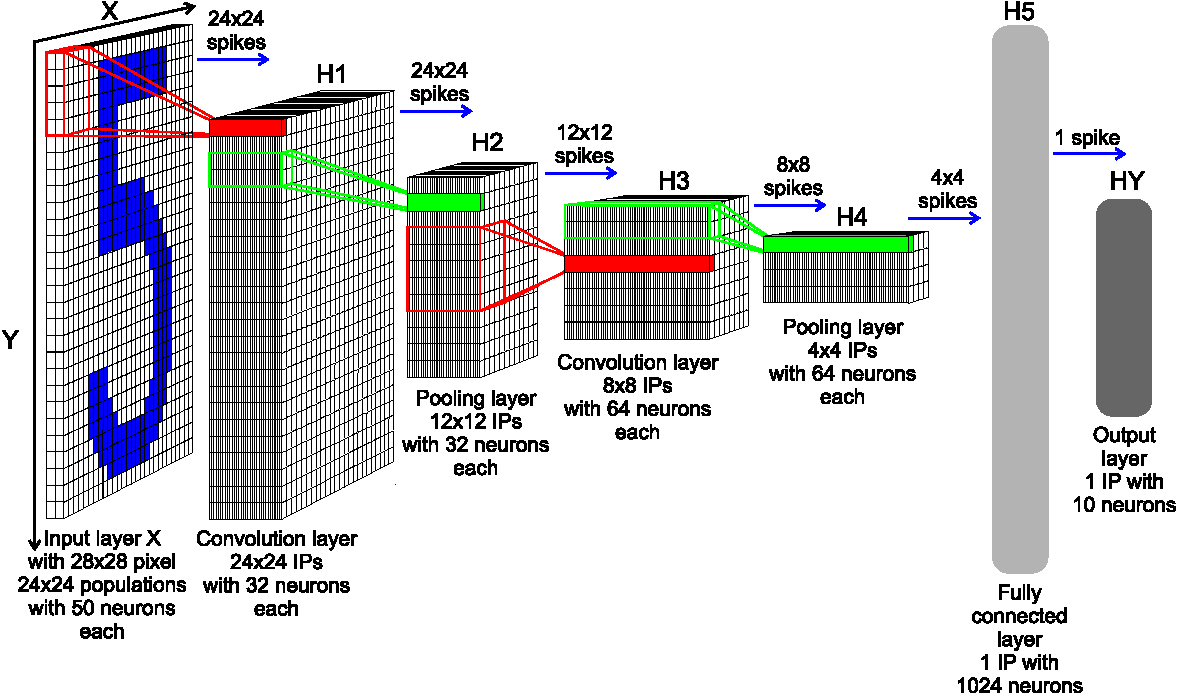
\includegraphics[width=0.5\columnwidth]{./chapters/sbs_accelerator/figures/sbs_network.pdf}
	\caption{\gls{sbs} network architecture for handwritten digit classification task.}
	\label{fig:sbs_network}
\end{figure*}


\begin{table}[t!]\centering
	\caption{\gls{sbs} network architecture for handwritten digit classification task.}
	\label{tab:sbs_network}
	\scriptsize
	\begin{tabular}{lrrrrrrr}\toprule
		&\multicolumn{3}{c}{\textbf{Layer size}} & &\multicolumn{2}{c}{\textbf{Kernel size}} \\\cmidrule{2-4}\cmidrule{6-7}
		\textbf{Layer} ($H^l$) &$N_X$ &$N_Y$ &$N_H$ & &$K_X$ &$K_Y$ \\\midrule
		Input ($HX$) &28 &28 &2 & &- &- \\
		Convolution ($H1$) &24 &24 &32 & &5 &5 \\
		Pooling ($H2$) &12 &12 &32 & &2 &2 \\
		Convolution ($H3$) &8 &8 &64 & &5 &5 \\
		Pooling ($H4$) &4 &4 &64 & &2 &2 \\
		Fully connected ($H5$) &1 &1 &1024 & &4 &4 \\
		Output ($HY$) &1 &1 &10 & &1 &1 \\
		\bottomrule
	\end{tabular}
\end{table}

\subsection{Computational Cost}

The number of \gls{mac} operations required for inference of an \gls{sbs} layer is defined by $NOPS_{MAC}=N_{Spk} N_X N_Y K_X K_Y (3 N_H + 2)$, where $N_{Spk}$ is the number of spikes (iterations), $N_X N_Y$ is the size of the layer, $K_X K_Y$ is the size of the kernel for convolution/pooling, and $N_H$ is the length of $\vec{h}$. The computational cost of \gls{sbs} network models is higher compared to equivalent \gls{cnn} models and lower compared to regular \gls{snn} models (e.g., \gls{lif}) \mbox{\cite{izhikevich2004model}}.


\begin{figure*}[b!]
	\centering
	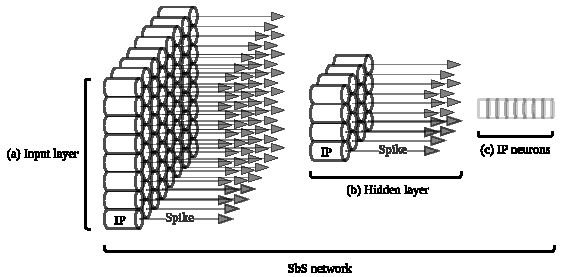
\includegraphics[width=0.5\columnwidth]{./chapters/sbs_accelerator/figures/SbS_layer.pdf}
	\caption{\gls{sbs} \gls{ip_sbs}s as independent computational entities, (a) illustrates an input layer with a massive amount of \glspl{ip_sbs} operating as independent computational entities, (b) shows a hidden layer with an arbitrary amount of \gls{ip_sbs}s as independent computational entities, (c) exhibits a set of neurons grouped in an \gls{ip_sbs}.}
	\label{fig:SbS_layer}
\end{figure*}


\subsection{Error Tolerance}

To illustrate the error tolerance/resilience of \gls{sbs} networks, we present a classification performance under positive additive uniformly distributed noise as external disturbance. \fig{fig:robustnes_sbs} presents a comparison of the classification performance of an \gls{sbs} network and a standard \gls{cnn}, with the same amount of
neurons per layer as well as the same layer structure. We trained both neural networks for handwritten digit classification on MNIST dataset \cite{lecun1998mnist} (see \cite{rotermund2019Backpropagation} for details). The figure shows the correctness for the MNIST test set with its \num[group-separator={,}]{10000} patterns in dependency of the noise level for positive additive
uniformly distributed noise. The blue curve shows the performance for
the \gls{cnn}, while the red curve shows the performance for
the \gls{sbs} network with \num[group-separator={,}]{1200} spikes (iterations). Beginning
with a noise level of 0.1, the respective performances are different
with a p - level of at least $10^{-6}$ (tested with the Fisher exact
test). Increasing the number of spikes per \gls{sbs} population to \num[group-separator={,}]{6000}
(performance values shown as black stars), shows that more spikes can
improve the performance under noise even more.

\begin{figure*}[b!]
	\centering
	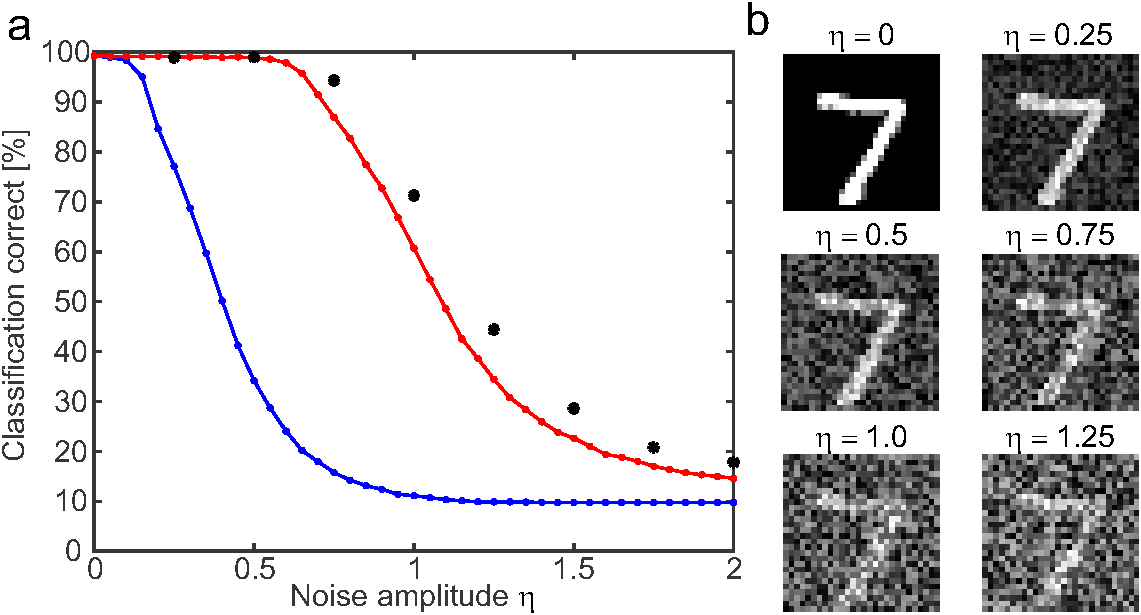
\includegraphics[width=0.5\columnwidth]{./chapters/sbs_accelerator/figures/sbs_robustnes.pdf}
	\caption{(a) Performance classification of \gls{sbs} NN versus equivalent \gls{cnn}, and (b) example of the first pattern in the MNIST test data set with different amounts of positive additive uniformly distributed noise.}
	\label{fig:robustnes_sbs}
\end{figure*}

%%%%%%%%%%%%%%%%%%%%%%%%%%%%%%%%%%%%%%%%%%%%%%%%%%%%%%%%%%%%%%%%%%%%%%%%%%%%%%%%%%%%%%
\section{Conv2D Tensor Operation}
A convolutional layer aims to learn feature representations from an input layer. The convolution layer is made of convolution kernels that are used to compute feature maps. Each unit of a feature map is connected to a region of neighboring units on the input maps (from previous layer). Such a neighborhood of the previous layer is known as the receptive field of the unit. A new feature map can be obtained by first convolving the input maps with a learned kernel and then applying a nonlinear elementwise activation function to the convolved results. All spatial locations on the input maps share a kernel to generate a feature map. All feature maps are obtained by convolving several different kernels~\cite{gu2018recent}.


The 2D convolution process is performed by the \emph{Conv2D} tensor operation, described in \Equ{eq:conv2D}, where $h$ is the input tensor containing the feature maps, $W$ is the convolution kernels (known as filters), and $b$ is the bias vector for the output feature maps~\cite{goodfellow2016deep}. $K\times L\times M$ is the receptive field size, $K\times L$ is the convolution kernel, and $M$ is the number of input channels/feature maps. We denote \emph{Conv} as \emph{Conv2D} operator.
\begin{eqnarray} \label{eq:conv2D}
Conv\left(W,h\right)_{i,j,o}=\sum_{k,l,m}^{K,L,M} h_{(i+k,j+l,m)} W_{(o,k,l,m)}+b_{o}
\end{eqnarray}

\section{Floating-point Number Representation}
The representation of every numerical value, in any number system, is made of an integer and a fractional part. The border that delimits them is called the radix point. The fixed-point format for representing numeric values derives its name from the fact that in this format, the base point is fixed at a certain position. For integer numbers, this position is at the right of the least significant digit.

In scientific computation, it is often necessary to represent very large and very small values. This is difficult to achieve using the fixed-point format because the bit size/width required to maintain both the desired precision and the desired range are very large. In such situations, \gls{fp} formats are used to represent real numbers. Each \gls{fp} number can be divided into three fields: sign $S$, exponent $E$, and mantissa $M$. Using the binary number system, it is possible to represent any \gls{fp} number as:

\begin{eqnarray} \label{eq:float}
(-1)^{S} \times 1.M \times 2^{E-B}
\end{eqnarray}

In \gls{fp} representations the exponent is biased. This bias depends on the bit size of the exponent field in the particular format. This exponent bias is defined by \Equ{eq:float_bias}, where $E_{size}$ is the exponent bit size.

\begin{eqnarray} \label{eq:float_bias}
B=2^{E_{size}-1}-1
\end{eqnarray}

There is a natural trade-off between small bit size requiring fewer hardware resources and larger bit size providing higher precision. Within a given total bit size, it is possible to assign various combinations of sizes to the exponent and mantissa fields, with wider exponents resulting in a higher range and wider mantissa resulting in better precision.

The most widely used format for \gls{fp} arithmetic is the IEEE 754 standard \cite{zuras2008ieee}. The IEEE single-precision format (32-bit) is expressed by \Equ{eq:float} with $B$ = 127, 8 bits for the exponent and 23 bits for the mantissa, see \Fig{fig:floating}(a). In \gls{fp} formats, the numbers are normalized, the leading one is an implicit bit, and only the fractional part is explicitly stored in the mantissa field.

\begin{figure*}[b!]
	\centering
	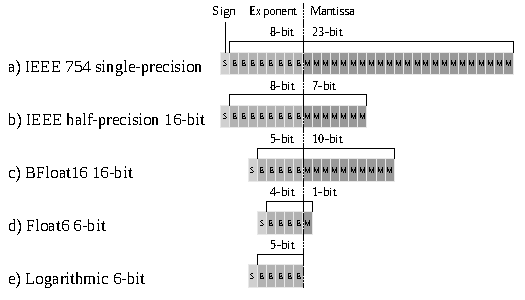
\includegraphics[width=0.5\columnwidth]{./chapters/cnn_accelerator/figures/power_breakdown/floating_point.pdf}
	\caption{Floating-point number representation.}
	\label{fig:floating}
\end{figure*}

Reduced bit size than those specified in the IEEE 754 standard are often sufficient to provide the desired precision. Reduced designs require fewer hardware resources enabling low-power implementations. In custom hardware designs, it is possible to customize the \gls{fp} format implemented. In later sections, we use the term E$a$M$b$ to denote \gls{fp} formats, where $a$ and $b$ are the exponent and mantissa bit size, respectively. For example, E4M1 means 4-bit exponent and 1-bit mantissa, see \Fig{fig:floating}(d).

There are three special definitions in IEEE 754 standard. The first is subnormal numbers when $E=0$, then \Equ{eq:float} is modified to \Equ{eq:float_subnorm}. Infinity and \gls{nan} are the other two special cases but are not used in our work.

\begin{eqnarray} \label{eq:float_subnorm}
(-1)^{S} \times 0.M \times 2^{1-B}
\end{eqnarray}
\chapter{Accelerating Spike-by-Spike Neural Networks} \label{chap.sbs}
\minitoc
\section{Introduction}
\label{sec:introduction}
%%% General intro
The exponential improvement in computing performance and the availability of large amounts of data are boosting the use of \gls{ai} applications in our daily lives. Among the various algorithms developed over the years, neural networks have demonstrated remarkable performance in a variety of image, video, audio, and text analytics tasks~\cite{schmidhuber2015deep,Taigman_2014_CVPR}. Historically, \glspl{ann} can be classified into three different generations \cite{Design_Exploration_SbS_Trans20}: the first one is represented by the classical McCulloch and Pitts neuron model using discrete binary values as outputs; the second one is represented by more complex architectures as \gls{mlp} and \gls{cnn} using continuous activation functions; while the third generation is represented by \gls{snn} using spikes as means for information exchange between groups of neurons. Although the \gls{ai} research is currently dominated by \glspl{dnn} from the second generation, the \glspl{snn} belonging to the third generation are receiving considerable attention \cite{Spinnaker_Trans13,ernst2007efficient,Design_Exploration_SbS_Trans20, SNN_Survey_Trans19}.

\glspl{snn} offer advantageous robustness and the potential to achieve a power efficiency closer to that of the human brain.
%%%
\glspl{snn} operate reliably using stochastic elements that are inherently non-reliable mechanisms \cite{mcdonnell2011benefits}.
This provides superior resistance against adversary attacks
\cite{ernst2007efficient, Dapello2020.06.16.154542}. Beside
robustness, \glspl{snn} have further advantages like the possibility of a more efficient asynchronous parallelization and higher
energy efficiency than \glspl{dnn}. For
example, Loihi \cite{davies2018loihi}, a \gls{snn} developed by Intel, can
solve LASSO optimization problems with an over three orders of
magnitude better energy-delay product than conventional
approaches. These advantages are motivating large research programs by
major companies (e.g., Intel \cite{davies2018loihi} and IBM
\cite{TrueNorth_Trans15}) as well as pan-european projects in the
domain of spiking networks \cite{Spinnaker_Trans13}.


\glspl{snn} emulate the real behavior of neurons in different levels of detail. The more detailed the biological part is emulated, the greater the computational complexity \cite{izhikevich2004model,amunts2019human}. For example, \gls{lif} is a widely used model; however, this model is relatively complex for emulation in embedded applications.
	
	Alternatively, the \gls{sbs} neural network is a remarkable model for its reduced complexity, which is on the less realistic side of the \gls{snn} scale of biological realism~\cite{rotermund2019Backpropagation,ernst2007efficient}. Consequently, the hardware complexity of \gls{sbs} network implementations is greatly reduced
	\cite{nevarez2020accelerator,rotermund2018massively}. In spite of this, \gls{sbs} still uses stochastic spikes as a means of transmitting information between populations of neurons and thus retains the advantageous robustness of \glspl{snn}.


%%% SbS intro
%SbS neural networks \cite{rotermund2019back,ernst2007efficient} are inspired by the %natural information processing of the mammalian brain.
The conceptual model in \gls{sbs} (see Chapter~\ref{sec:sbs} for a review) differs fundamentally from conventional \glspl{ann} since (a) the building blocks of the network are \glspl{ip_sbs} which are an optimized generative representation with non-negative values, (b) time progresses from one spike to the next, preserving the property of stochastically firing neurons, and (c) a network has only a small number of parameters, which is an advantageous noise-robust stochastic version of \gls{nnmf}. The \gls{sbs} network is placed between non-spiking \glspl{nn} and stochastically spiking \glspl{nn}, which offers advantages from both structures \cite{rotermund2019Backpropagation}. On one hand, the \gls{sbs} model incorporates the inherent robustness of \glspl{snn}, which provide the possibility of more efficient asynchronous parallelization and superior resilience against disturbances based on the synaptic stochasticity; on the other hand, the \gls{sbs} model incorporates the regular flow of information from \glspl{cnn}, which are expressed on explicit vector operations.  


%%%%%%% Problem statement
As computational demanding algorithms, \glspl{cnn} and \glspl{snn} in particular, must be addressed by specialized hardware architectures. A significant research effort has been performed in \gls{snn} accelerators, see e.g.~\cite{roy2019towards,bouvier2019spiking, young2019review,TrueNorth_Trans15,Spinnaker_Trans13,davies2018loihi}.
  However, hardware accelerators that focus on \gls{sbs} have only been partially investigated so far~\cite{nevarez2020accelerator,rotermund2018massively}.
  Enhanced \gls{sbs} accelerators will have a double impact. From the application point of view, they will contribute to the deployment of robust neural networks in small embedded systems~\cite{nevarez2020accelerator}; from the scientific point of view, they will facilitate fundamental research for neuroscience~\cite{ernst2007efficient,rotermund2019recurrentsbs, dayan2001theoretical}.

A central point that can be optimized in current \gls{sbs} accelerators
is the use of approximation techniques.
Most \gls{sbs} models use \gls{fp}  numerical representation, which imposes high complexity of the required circuits for the \gls{fp} operations. Model quantization has the potential to improve computational performance; however, this solution is often accompanied by quantization-aware training methods that, in some cases, are problematic or even inaccessible, particularly in deep \gls{snn} algorithms~\cite{zhang2018survey}. 
As an alternative, based on the relaxed need for fully precise or deterministic computation of neural networks, approximate computing techniques allow substantial enhancement in processing efficiency with moderated accuracy degradation. Some research papers have shown the feasibility of applying approximate computing to the inference stage of neural networks~\cite{lotrivc2012applicability, sarwar2016multiplier, mrazek2016design, du2014leveraging}. Such techniques usually demonstrated small inference accuracy degradation, but significant enhancement in computational performance, chip-area, and energy consumption. Hence, by taking advantage of the intrinsic error-tolerance of neural networks, approximate computing is positioned as a promising approach for inference on resource-limited devices.

\begin{figure*}[b!]
	\centering
	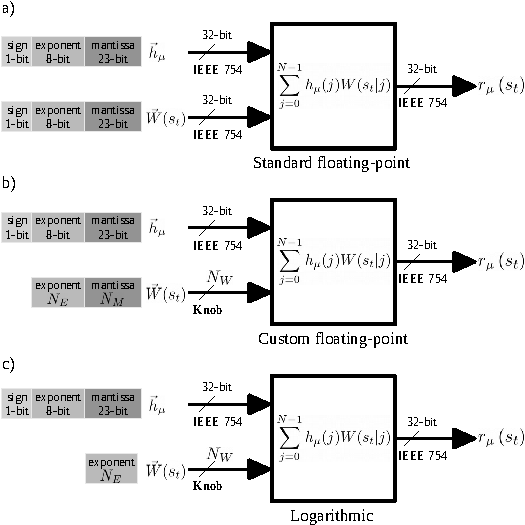
\includegraphics[width=0.5\columnwidth]{./chapters/sbs_accelerator/figures/dot-product_unit.pdf}
	\caption{Dot-product hardware module with (a) standard floating-point (IEEE 754) arithmetic, (b) hybrid custom floating-point approximation, and (c) hybrid logarithmic approximation.}
	\label{fig:dot_product_unit}
\end{figure*}

%%%%%%% Contributions
In this chapter, we accelerate \gls{sbs} neural networks with a dot-product hardware design based on approximate computing with hybrid custom \gls{fp}  and logarithmic number representation. This hardware unit has a quality configurable scheme based on the bit truncation of the synaptic-weight vector. \Fig{fig:dot_product_unit} illustrates the dot-product hardware module with standard \gls{fp} (IEEE 754) arithmetic, and our approach with hybrid custom \gls{fp}  as well as logarithmic approximation. As a design parameter, the mantissa bit-width of the weight vector provides a tunable knob to trade-off between efficiency and \gls{qor}~\cite{park2009dynamic, han2013approximate}. Since the lower-order bits have smaller significance than the higher-order bits, truncating them may have only a minor impact on \gls{qor}~\cite{gupta2011impact, mittal2016survey}. Further on, we can remove completely the mantissa bits in order to use only the exponent of a \gls{fp}  representation. Therefore, the most efficient setup and yet the worst-case quality configuration becomes a logarithmic representation, which consequently leads to significant architectural-level optimizations using only adders and shifters for dot-product approximation in hardware. Moreover, since approximations and noise have qualitatively the same effect~\cite{venkataramani2015approximate}, we apply noise tolerance plots as an intuitive visual measure to provide insights into the quality degradation of \gls{sbs} networks under approximate processing effects.

The main contributions in this work are as follows:

\begin{itemize}
	\item We develop a hardware component for dot-product approximation. To perform the sum of pairwise products of two vectors, this hardware module has the following three design features: (1) the pairwise product is approximated by adding integer exponents and multiplying truncated mantissas, and the sum of products is done by accumulating denormalized integer products with barrel shifters, which increases computational throughput; (2) the synaptic weight vector uses either reduced custom \gls{fp} or logarithmic representation, which reduces memory footprint; and (3) the neuron vector uses either standard or custom \gls{fp} representation, which preserves \gls{qor} and overall inference accuracy.
	\item We address a hardware design exploration with the proposed dot-product approximation using synaptic weight vectors with custom \gls{fp} and logarithmic representation as shown in \Fig{fig:dot_product_unit}. We evaluate inference run-time, accuracy degradation, resource utilization and power dissipation. Experimental results demonstrate $20.5\times$ run-time enhancement versus embedded CPU (ARM Cortex-A9 at \unit[666]{MHz}), and less than $0.5\%$ of accuracy degradation without retraining on a handwritten digit recognition task (MNIST). This machine learning task simply provides a proof of concept to demonstrate the feasibility of our approximation technique for \gls{sbs} neural network accelerators.
	\item We propose a noise tolerance plot as quality monitor, which serves as an intuitive visual model to provide insights into the accuracy degradation of \gls{sbs} networks under approximate processing effects.
	\item Our proposed design for dot-product approximation is adaptable as a building block for other error resilient applications (e.g., image/video processing).
\end{itemize}

To promote the research on \gls{sbs} networks, our design exploration framework is made available to the public as an open-source project at https://github.com/YaribNevarez/sbs-framework.git


\section{Related Work}
\label{sec:related_work}
%%%%%%%%%%%%%%%%%%%%%%%%%%%%%%%%%%%%%%%%%%%%%%%%%%%%%%
For efficient neural network computation, two main optimization strategies are used, namely network compression and classical approximate computing~\cite{bouvier2019spiking}.

\subsection{Network Compression}
Researchers focusing on embedded applications started lowering the precision of weights and activation maps to shrink the memory footprint of the large number of parameters representing \glspl{ann}, a method known as network compression or quantization. This practice takes advantage of the intrinsic error-tolerance of neural networks, as well as their ability to compensate for approximation while training. In this way, reduced bit precision causes a small accuracy loss~\cite{courbariaux2015binaryconnect, han2015deep, hubara2017quantized, rastegari2016xnor}.

In hardware development, \gls{wq} has shown up to $2\times$ improvement in energy consumption with an accuracy degradation of less than $1\%$ \cite{moons20160, whatmough201714}. Some advanced quantization methods yield to \glspl{bnn} allowing the use of \glspl{xnor} instead of the conventional costly \glspl{mac}~\cite{rastegari2016xnor}. In~\cite{sun2018xnor}, Sun et al. report an accuracy of $98.43\%$ on handwritten digit classification (MNIST) with a simple \gls{bnn}. Hence, quantization is a powerful tool for improving the energy efficiency and memory requirements of \gls{ann} accelerators, with limited accuracy degradation.

In addition to quantization, network pruning reduces the model size by removing structural portions of the parameters and its associated computations~\cite{lecun1989optimal,hassibi1992second}. This method has been identified as an effective technique to improve the efficiency of \gls{dnn} for applications with limited computational budget~\cite{molchanov2016pruning,li2016pruning, liu2018rethinking}.

These methods can be used for \glspl{snn} as well. In~\cite{rathi2018stdp}, Rathi et al. report up to $3.1\times$ improvement in energy consumption with an accuracy loss of around $3\%$. Weight quantization allows the designer to realize a trade-off between the accuracy of the \gls{snn} application and efficiency of resources. Approximate computing can also be applied at the neuron level, where irrelevant units are deactivated to reduce the computation cost of the \glspl{snn}~\cite{sen2017approximate}. This computation skipping can be applied randomly on synapses, training \glspl{ann} with stochastic synapses improves generalization, resulting in a better accuracy~\cite{srivastava2014dropout, wan2013regularization}. Such methods are compatible with \glspl{snn} and have been tested both during training~\cite{neftci2016stochastic, srinivasan2016magnetic} and operation \cite{buesing2011neural}, and even to define the connectivity between layers \cite{bellec2017deep, chen20184096}. Implementations of spiking neuromorphic systems in FPGA~\cite{sheik2016synaptic} and hardware~\cite{jerry2017ultra} demonstrated that synaptic stochasticity allows to increase the final accuracy of the networks while reducing memory footprint.

Quantization is therefore a powerful technique to improve energy efficiency and memory requirements of \gls{ann} and \gls{snn} accelerators, with small accuracy degradation. However, this approach requires quantization-aware training methods that, in some cases, are problematic or even inaccessible, particularly in emerging deep \gls{snn} algorithms~\cite{zhang2018survey}.

\subsection{Classical Approximate Computing}
Approximate computing has been used in a wide range of applications to increase the computational efficiency in hardware\cite{han2013approximate}. This approach consists of designing processing elements that approximate their computation by employing modified algorithmic logic units \cite{han2013approximate}. In~\cite{kim2013energy}, Kim et al. have shown \glspl{snn} using carry skip adders achieving $2.4\times$ latency enhancement and $43\%$ more energy efficiency, with an accuracy degradation of 0.97\% on a handwritten digit classification task (MNIST). Therefore, approximate computing provides important enhancement in energy efficiency and processing speed.

However, as the complexity of the dataset increases, as well as the depth of the network topology, such as ResNet~\cite{he2016deep} on ImageNet~\cite{russakovsky2015imagenet}, the accuracy degradation becomes more important and may not be negligible anymore \cite{rastegari2016xnor}, especially for critical applications such as autonomous driving. Therefore, it is not certain that network compression techniques and approximate computing are suitable for all applications.

\subsection{Spike-by-Spike Neural Networks Accelerators}
Recently, Rotermund et al. demonstrated the feasibility of a neuromorphic \gls{sbs} \gls{ip_sbs} on a Xilinx Virtex 6 \gls{fpga}~\cite{rotermund2018massively}. It provides a massively parallel architecture, optimized to reduce memory access and suitable for \gls{asic} implementations. Nonetheless, this design is considerably resource-demanding if implemented as a full \gls{sbs} network in today's embedded technology.
%%%%%%%%%%%%%%%%%%%%%%%%%%%%%%%%%%%%%%%%%%%%%%%%%%%%%%
\section{System Design}
\label{sec:system_design}

	In this section, we present a hardware architecture composed of specialized heterogeneous \glspl{pu} with hybrid custom floating-point and logarithmic dot-product approximation. This approach represents an advantageous design for error resilient applications in resource-constrained devices due to the reduced computational costs and memory footprint. Furthermore, the proposed approach allows the implementation of stationary synaptic weight matrices.
	

Regarding the software architecture, this is structured as a
layered object-oriented application framework written in the C programming language. This offers a comprehensive high level embedded software \gls{api} that allows the construction of scalable sequential SbS networks with configurable hardware acceleration. Conceptually this design is modular, reusable, and extensible. The overall structure is depicted in \Fig{fig:sbs_sw_stack}.

\begin{figure*}[b!]
	\centering
	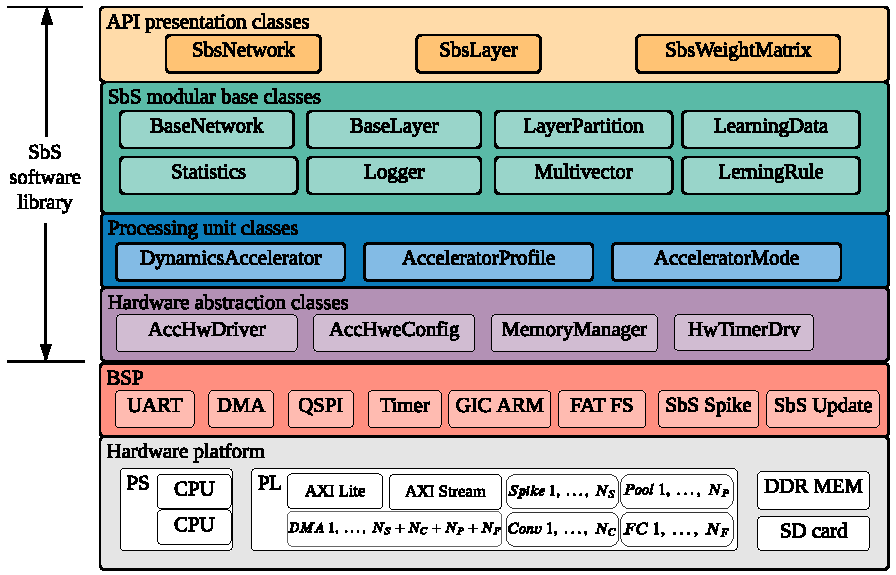
\includegraphics[width=0.5\columnwidth]{./chapters/sbs_accelerator/figures/sbs_software_component.pdf}
	\caption{System-level overview of the embedded software architecture.}
	\label{fig:sbs_sw_stack}
\end{figure*}

\subsection{Hardware Architecture} \label{Hardware_architecture}
As a hardware/software co-design, the system architecture is an embedded CPU+FPGA-based platform, where the acceleration of SbS network computation is based on asynchronous\footnote{The system is synchronous at the circuit level, but the execution is asynchronous in terms of jobs.} execution of parallel heterogeneous processing units: \emph{Spike} (input layer), \emph{Conv} (convolution), \emph{Pool} (pooling), and \emph{FC} (fully connected). \Fig{fig:hw_sbs} illustrates the system overview as a scalable structure. For hyperparameter configuration, each PU uses AXI-Lite interface. For data transfer, each \gls{pu} uses AXI-Stream interfaces via \gls{dma} allowing data movement with high transfer rate. Each \gls{pu} asserts an interrupt flag once the job or transaction is complete. This interrupt event is handled by the embedded \gls{cpu} to collect results and start a new transaction.

The hardware architecture can resize its resource utilization by changing the number of PUs instances prior to the hardware synthesis, this provides scalability with a good trade-off between area and throughput. The dedicated PUs for \emph{Conv} and \emph{FC} implement the proposed dot-product approximation as a system component. The PUs are written in C using Vivado \gls{hls}. In this research, we illustrate the integration of the approximate dot-product component on the \emph{Conv} \gls{pu}.

\begin{figure*}[b!]
	\centering
	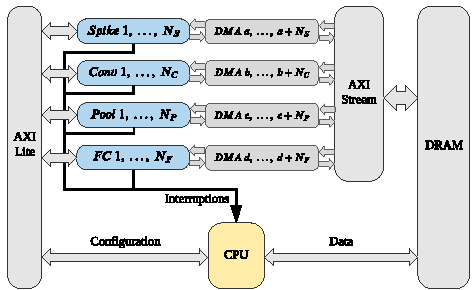
\includegraphics[width=0.5\columnwidth]{./chapters/sbs_accelerator/figures/sbs_hw.pdf}
	\caption{System-level hardware architecture with scalable number of heterogeneous \glspl{pu}: \emph{Spike}, \emph{Conv}, \emph{Pool}, and \emph{FC}}
	\label{fig:hw_sbs}
\end{figure*}

\subsection{Conv Processing Unit}
This hardware module computes the \gls{ip_sbs} dynamics defined by \Equ{eq:sbs_update} and offers two modes of operation: \emph{configuration} and \emph{computation}.

\subsubsection{Configuration Mode}
In this mode of operation, the \gls{pu} receives and stores in on-chip memory (BRAM) the hyperparameters to compute the \gls{ip_sbs} dynamics: $\epsilon$ as the epsilon, $N$ as the length of $\vec{h}_\mu\in\mathbb{R}^{N}$, $K\in\mathbb{N}$ as the size of the convolution kernel, and $H\in\mathbb{N}$ as the number of \glspl{ip_sbs} to process per transaction. $H$ is the number of \glspl{ip_sbs} forming a layer or a partition.

Additionally, the processing unit also stores in on-chip memory (BRAM) the synaptic weight matrix using a number representation with a reduced memory footprint. Fundamentally, the synaptic weight matrix is defined by $W\in\mathbb{R}^{K\times K\times M\times N}$ with $0\le W(s_t|j)\le1$ and $\sum_{s_t=0}^{M-1}W(s_t|j)=1$ \cite{rotermund2019Backpropagation}. Hence, $W$ employs only positive normalized real numbers. Therefore, $W$ is deployed using a reduced floating-point or logarithmic representation as follows:

\begin{itemize}
	\item{Custom floating-point representation}.
	In this case, $W$ is deployed with a reduced floating-point representation using the user defined bit-width for the exponent and for the mantissa. For example, 4-bit exponent, 1-bit mantissa; as a result: 5-bit custom floating-point. The proposed method to determine the required bit-width is described in Section~{\ref{sec:dot-product_hardware_module}}.
	\item{Logarithmic representation}.
	In this case, the synaptic weight matrix is $W\in\mathbb{N}^{K\times K\times M\times N}$ with positive natural numbers. Since $0\le W(s_t|j)\le1$ and $\sum_{s_t=0}^{M-1}W(s_t|j)=1$, $W$ has only negative values in the logarithmic domain. Hence, the sign bit is omitted, and the values are represented in its positive form. Therefore, $W$ is deployed with a representation using the necessary bit-width for the exponent according to the given application. For example, 4-bit exponent. The method to determine the required bit-width is described in Section~{\ref{sec:dot-product_hardware_module}}.
\end{itemize}

In order to deploy different SbS models, the \emph{Conv} processing units can load different hyperparameters and synaptic weight matrices as required through the embedded software.

\subsubsection{Computation Mode}
In this mode of operation, the \gls{pu} executes a transaction to process a group of \glspl{ip_sbs} using the previously given hyperparameters and synaptic weight matrix. This process operates in six stages as shown in \fig{fig:hw_conv}. In the first two stages, the \gls{pu} receives $\vec{h}_\mu\in\mathbb{R}^{N}$, then the \gls{pu} calculates the emitted spike and stores it in $S^{new}\in\mathbb{N}^{H}$ (output spike vector). From the third to the fifth stage, the \gls{pu} receives $S_t\in\mathbb{N}^{K\times K}$ (input spike matrix), then it computes the update dynamics, and then it dispatches $\vec{h}_\mu^{new}\in\mathbb{R}^{N}$ (updated \gls{ip_sbs}). This process repeats for $H$ number of loops (for each \gls{ip_sbs} of the layer or partition). Finally, the $S^{new}$ is dispatched.

The computation of the update dynamics (see \fig{fig:hw_conv}(d)) operates in two modular stages: \emph{dot-product} and \emph{neuron update}. First, the \emph{dot-product} module calculates the sum of pairwise products of $\vec{h}_{\mu}$ and $\vec{W}(s_t)$, each pairwise product is stored as intermediate results. Subsequently, the \emph{neuron update} module calculates \equ{eq:sbs_update} reusing parameters and previous results.


The calculation of the dot-product of \equ{eq:sbs_update} represents a considerable computational cost using standard floating-point in non-quantized network models. Fortunately, the pair product of $h_{\mu}(j)$ and $W(s_t|j)$ was defined by us as an approximable factor in the dot-product of \equ{eq:sbs_update}. In the following section, we focus on an optimized dot-product hardware design based on approximate computing.


\begin{figure*}[b!]
	\centering
	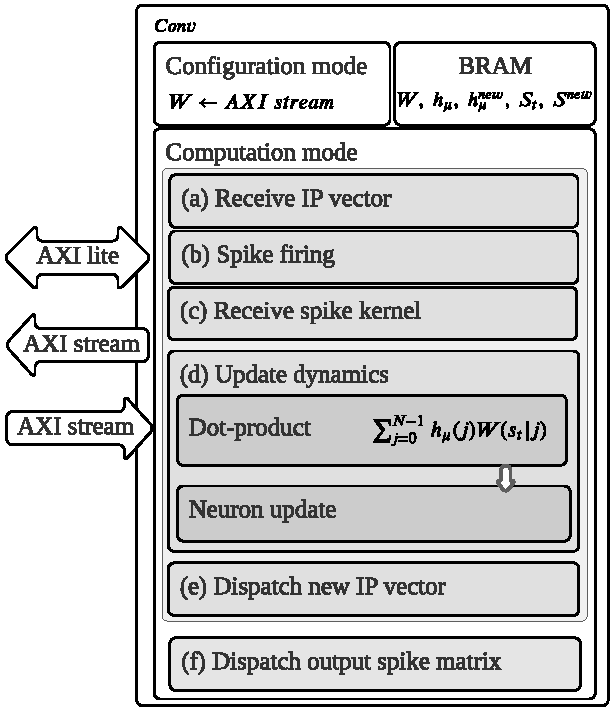
\includegraphics[width=0.5\columnwidth]{./chapters/sbs_accelerator/figures/sbs_conv.pdf}
	\caption{The \emph{Conv} processing unit and its six stages: (a) receive \gls{ip_sbs} vector, (b) spike firing, (c) receive spike kernel, (d) update dynamics, (e) dispatch new \gls{ip_sbs} vector, (f) dispatch output spike matrix.}
	\label{fig:hw_conv}
\end{figure*}

\subsection{Dot-Product Hardware Module}
\label{sec:dot-product_hardware_module}
This dot-product hardware module is part of an application-specific architecture optimized to approximate the dot-product of arbitrary length vectors, see \equ{eq:dot_product}. For quality configurability, we parameterized the mantissa bit-width of $\vec{W}(s_t)$, which provides a tunable trade-off between resource utilization and \gls{qor}. Since the lower-order bits have smaller significance than the higher-order bits, removing them may have only a minor impact on \gls{qor}. We designate this as hybrid custom floating-point approximation (see {\fig{fig:dot_product_unit}}(b)).

\begin{eqnarray} \label{eq:dot_product}
r_{\mu}\left(s_t\right)=\sum_{j=0}^{N-1}h_{\mu}(j)W(s_t|j)
\end{eqnarray}

Further on, we remove the mantissa bits completely in order to use only the exponent of a floating-point representation. Hence, the worst-case quality and yet the most efficient configuration becomes a logarithmic representation. Consequently, this structure leads to advantageous architectural optimizations using only adders and barrel shifters for dot-product approximation in hardware. We designate this as hybrid logarithmic approximation (see {\fig{fig:dot_product_unit}}(c)).

In order to determine the required bit-width for the number representation, we use {\equ{eq:exp_max}}, {\equ{eq:bits_exp}}, and {\equ{eq:bits_bitwidth}}.

\begin{eqnarray} \label{eq:exp_max}
E_{\min}=\log _2(\min_{\forall i}(W(i)))
\end{eqnarray}

\begin{eqnarray} \label{eq:bits_exp}
N_E=\lceil\log_2(|E_{\min}|)\rceil
\end{eqnarray}

\begin{eqnarray} \label{eq:bits_bitwidth}
N_W=N_E + N_M
\end{eqnarray}


The \equ{eq:exp_max} obtains the exponent of the minimum entry value in the synaptic weight matrix. Since $0\le W(s_t|j)\le1$ and $\sum_{s_t=0}^{M-1}W(s_t|j)=1$, $W$ has only negative values in the logarithmic domain; hence, by searching for the smallest value, we obtain the biggest negative exponent ($E_{\min}$). Then, the {\equ{eq:bits_exp}} obtains the necessary bit-width to represent the exponent ($N_E$). Finally, we obtain the total bit-width by incorporating both exponent and mantissa bit-widths in {\equ{eq:bits_bitwidth}}. $N_M$ denotes the mantissa bit-width, this is a knob parameter that is tuned by the designer to trade-off between resource utilization and \gls{qor}. The bit-width concept is illustrated in {\fig{fig:dot_product_unit}}.

In this section, we will present three pipelined hardware modules with standard floating-point (IEEE 754) computation, hybrid custom floating-point approximation, and hybrid logarithmic approximation.

\subsubsection{Dot-Product with Standard Floating-Point Computation}
 The hardware module to calculate the dot-product with standard floating-point computation is shown in \Fig{fig:dot_product_float}. This diagram presents the hardware blocks and their clock cycle schedule. This module loads both $h_\mu(j)$ and $W(s|j)$ from BRAM, then the \gls{pu} executes the pairwise product (\Fig{fig:dot_product_float}(c)) and accumulation (\Fig{fig:dot_product_float}(d)). The intermediate results of $h_\mu(j) W(s_t|j)$ are stored in BRAM for reuse in the neuron update. The latency in clock cycles of this hardware module is defined by \Equ{eq:dot_standard_float_latency}, where $N$ is the vector length of the dot-product. This equation is obtained from the general pipelined hardware latency formula: $L=\left(N-1\right)II+IL$, where $II$ is the initiation interval (\Fig{fig:dot_product_float}(a)), and $IL$ is the iteration latency (\Fig{fig:dot_product_float}(b)). Both $II$ and $IL$ are obtained from the high-level synthesis analysis. The equation for the latency with standard 32-bit floating-point is:
 \begin{eqnarray} \label{eq:dot_standard_float_latency}
 L_{f32}=10N+9
 \end{eqnarray}
 
In this design, the high-level synthesis tool infers computational blocks with considerable latency cost for standard floating-point. In the case of floating-point multiplication (\Fig{fig:dot_product_float}(c)), the synthesis infers a hardware block with a latency cost of 5 clock cycles. Theoretically, this block would handle exponents addition, mantissas multiplication, and mantissa correction if needed. Moreover, in the case of floating-point addition (\ref{fig:dot_product_float}(d)), the synthesis infers a hardware block with a latency cost of 9 clock cycles. Seemingly, this block would handle mantissas alignment, addition, and correction if needed. Therefore, the use of standard floating-point in high-level synthesis results in high computational cost, which represents unnecessary overhead in error tolerant applications.


\begin{figure*}[b!]
	\centering
	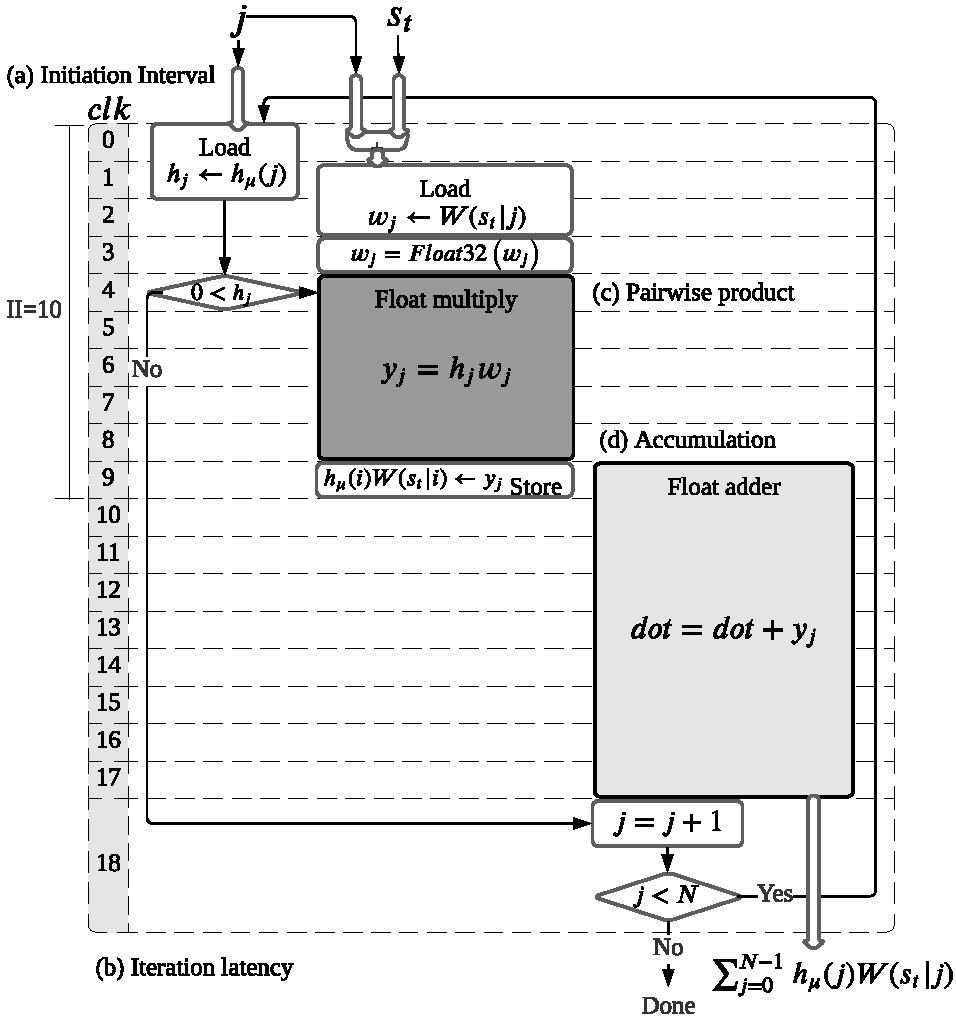
\includegraphics[width=0.5\columnwidth]{./chapters/sbs_accelerator/figures/dot_product_float.pdf}
	\caption{Dot-product hardware module with standard floating-point (IEEE 754) computation, (a) exhibits the initiation interval of 10 clock cycles, (b) presents the iteration latency of 19 clock cycles, (c) shows the pairwise product block in dark-gray, and (d) illustrates the accumulation block in light-gray.}
	\label{fig:dot_product_float}
\end{figure*}

\subsubsection{Dot-Product with Hybrid Custom Floating-Point and Logarithmic Approximation}
 The hardware module to calculate dot-product with hybrid custom floating-point approximation is shown in \Fig{fig:dot_product_custom}. In this design, $h_\mu(j)$ uses standard 32-bit floating-point number representation, and $W(s|j)$ uses a positive reduced custom floating-point number representation, where the mantissa bit width is the quality configurability knob. This parameter is tuned by the designer to trade-off between QoR and resource utilization, thus, energy consumption.
 
 As the most efficient setup and yet the worst-case quality configuration, by completely truncating the mantissa of $W(s|j)$ leads to a slightly different hardware architecture using only adders and shifters, which computes the dot-product with hybrid logarithmic approximation. This is shown in \Fig{fig:dot_product_log}.
 
Additionally, the exponent bit-width of $W(s|j)$ is a design parameter for efficient resource utilization and it is defined based on the application or deployment needs.
 
 The hybrid custom floating-point and logarithmic approximation designs work in three phases: \emph{Computation}, \emph{Threshold-test}, and \emph{Result normalization}.
 
 \begin{itemize}
 	\item{Phase I, \emph{Computation}}: 
 	\\This phase approximates the magnitude of the dot-product in a denormalized representation. This is calculated in two iterative steps over each vector element: \emph{pairwise product} and \emph{accumulation}, where \emph{pairwise product} is executed either in hybrid custom floating-point or hybrid logarithmic approximation described below.
 	 \begin{itemize}[label={--}]
 	 	\item{Pairwise product}.
 	 	\begin{itemize} [label={--}]
	 		\item{Hybrid custom floating-point approximation}.
	 	 	As shown in \Fig{fig:dot_product_custom}(c) in dark-gray, the pairwise product is approximated by adding exponents and multiplying mantissas of both $W(s|i)$ and $h_\mu(i)$. If the mantissa multiplication results in an overflow, then it is corrected by increasing the  exponent and shifting the resulting mantissa by one position to the right. Then we get $h_\mu(j) W(s_t|j)$ as an intermediate result which is stored for future reuse in the neuron update calculation. In this design the pairwise product has a latency of 5 clock cycles.
	 	 	\item{Hybrid logarithmic approximation}.
	 	 	As shown in \Fig{fig:dot_product_log}(c) in dark-gray, the pairwise product is approximated by adding $W(s|i)$ to the exponent of $h_\mu(i)$, since $W(s|j)$ values are represented in the logarithmic domain and $h_\mu(j)$ in standard floating-point. In this design the pairwise product has a latency of one clock cycle.
 	 	\end{itemize}
 		\item{Accumulation}. As shown in both \Fig{fig:dot_product_custom}(d) and \Fig{fig:dot_product_log}(d) in light-gray, first, it is obtained the denormalized representation of $h_\mu(j) W(s_t|j)$ by shifting its mantissa using its exponent as shifting parameter (barrel shifter). Then, this denormalized representation is accumulated to obtain the approximated magnitude of the dot-product.
 	 \end{itemize}
 	The process of pairwise product and accumulation iterates over each element of the vectors. The computation latency is given by \Equ{eq:dot_standard_custom_float_latency} for hybrid custom floating-point, and \Equ{eq:dot_log_latency} for hybrid logarithmic, where $N$ is the length of the vectors. Both pipelined hardware modules have the same throughput, since both have two clock cycles as initiation interval. 	
 	\begin{eqnarray} \label{eq:dot_standard_custom_float_latency}
 	L_{custom}=2N+11
 	\end{eqnarray} 	
	\begin{eqnarray} \label{eq:dot_log_latency}
 	L_{log}=2N+7
 	\end{eqnarray}
 	
 	\item{Phase II, \emph{Threshold-test}}: \\
	The accumulated denormalized magnitude is tested to be above of a predefined threshold, it must be above zero, since the dot-product is the denominator in \Equ{eq:sbs_update}.
 	If passing the threshold, then the next phase is executed. Otherwise the rest of update dynamics is skipped. The threshold-test takes one clock cycle.
 	\item{Phase III, \emph{Result-normalization}}: \\
 	In this phase, the dot-product is normalized to obtain the exponent and mantissa in order to convert it to standard floating-point for later use in the neuron update. The normalization is obtained by shifting the approximated dot-product magnitude in a loop until it is in the form of a normalized mantissa where the iteration count represents the exponent of the dot-product. Each iteration takes one clock cycle.
 	
 \end{itemize}

The total latency of the hardware module with hybrid custom floating-point and hybrid logarithmic approximation is the accumulated latency of the three phases.

The proposed architectures with approximation approach exceeds the performance of the design with standard floating-point. This performance enhancement is achieved by decomposing the floating-point computation into an advantageous handling of exponent and mantissa using intermediate accumulation in a denormalized representation and only one final normalization.

\begin{figure*}[h!]
	\centering
	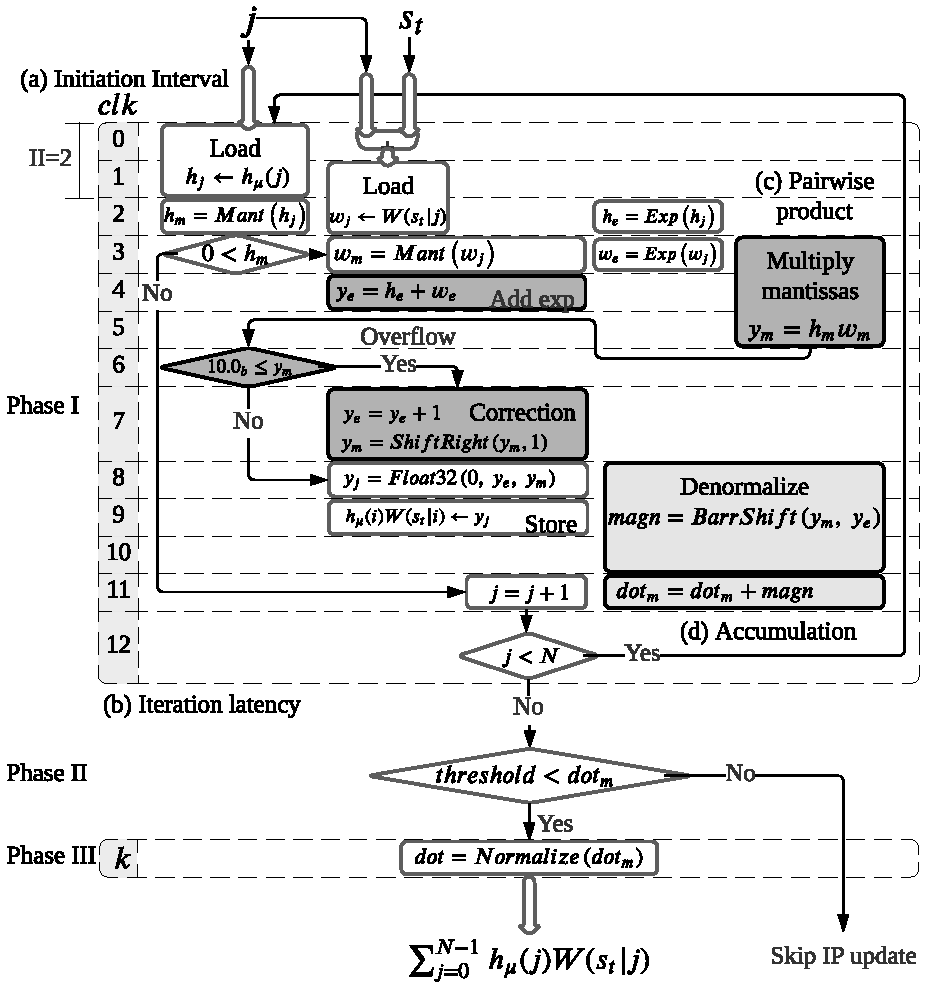
\includegraphics[width=0.5\columnwidth]{./chapters/sbs_accelerator/figures/dot_product.pdf}
	\caption{Dot-product hardware module with hybrid custom floating-point approximation, (a) exhibits the initiation interval of 2 clock cycles, (b) presents the iteration latency of 13 clock cycles, (c) shows the pairwise product blocks in dark-gray, and (d) illustrates the accumulation blocks in light-gray.}
	\label{fig:dot_product_custom}
\end{figure*}

\begin{figure*}[h!]
	\centering
	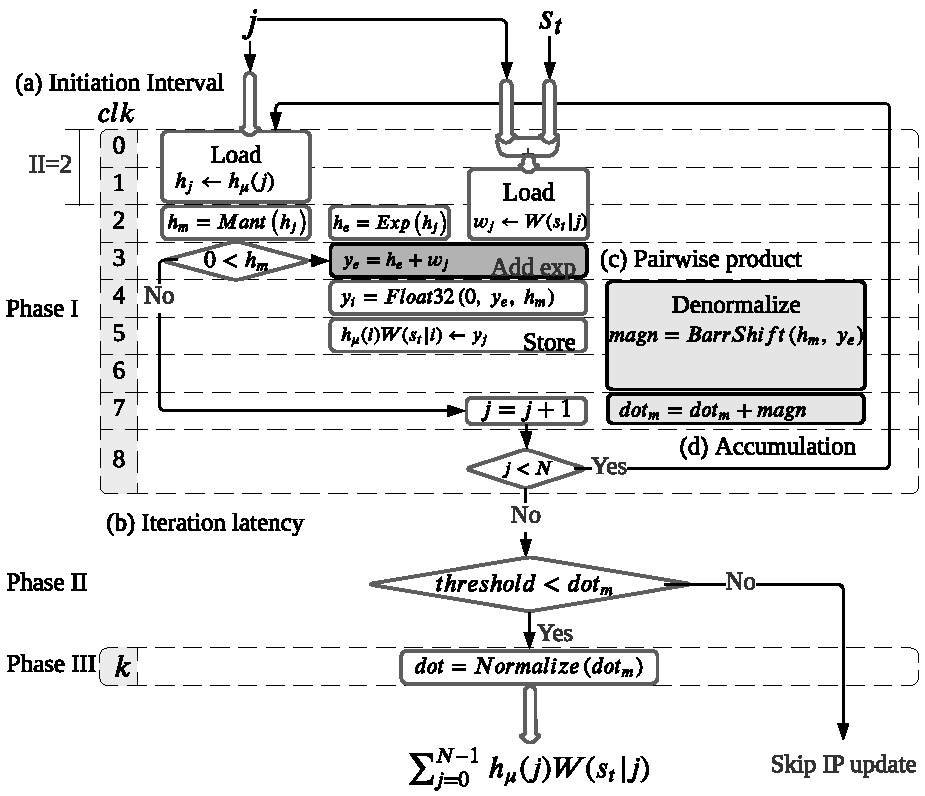
\includegraphics[width=0.5\columnwidth]{./chapters/sbs_accelerator/figures/dot_product_log.pdf}
	\caption{Dot-product hardware module with hybrid logarithmic approximation, (a) exhibits the initiation interval of 2 clock cycles, (b) presents the iteration latency of 9 clock cycles, (c) shows the pairwise product block in dark-gray, and (d) illustrates the accumulation blocks in light-gray.}
	\label{fig:dot_product_log}
\end{figure*}



\section{Experimental Results}
\label{sec:experimental_results}
The proposed architecture is demonstrated on a Xilinx Zynq-7020. This device integrates a dual ARM Cortex-A9 based \gls{ps} and \gls{pl} equivalent to Xilinx Artix-7 (FPGA) in a single chip \cite{xilinx2015zynq}. The Zynq-7020 architecture conveniently maps the custom logic and software in the PL and PS respectively as an embedded system.

In this platform, we implement the proposed hardware architecture to deploy the SbS network structure shown in \ref{fig:sbs_network} for handwritten digit classification task using MNIST data set. The SbS model is trained in Matlab without any quantization method, using standard floating-point. The resulting synaptic weight matrices are deployed on the embedded system. There, the SbS network is built as a sequential model using the API from the SbS embedded software framework \cite{nevarez2020accelerator}. This API allows to configure the computational workload of the neural network, which can be distributed among the hardware processing units and the embedded CPU.

For the evaluation of our approach, we address a design exploration by reviewing the computational latency, inference accuracy, resource utilization, and power dissipation. First, we benchmark the performance of SbS network simulation on the embedded CPU, and then repeat the measurements on hardware processing units with standard floating-point computation. Afterwards, we evaluate our dot-product architecture, addressing a design exploration with hybrid custom floating-point approximation, as well as the hybrid logarithmic approximation. Finally, we present a discussion of the presented results.


\subsection{Performance Benchmark}
\subsubsection{Benchmark on Embedded CPU}

We examine the performance of the CPU for SbS network simulation with no hardware coprocessing. In this case, the embedded software builds the SbS network as a sequential model mapping the entire computation to the CPU (ARM Cortex-A9) at 666 MHz and a power dissipation of $1.658 W$.

The SbS network computation on the CPU achieves a latency of $34.28 ms$ per spike with an accuracy of 99.3\% correct classification on the $10,000$ image test set with $1000$ spikes. The latency and schedule of the SbS network computation are displayed in \ref{tab:latency_sw} and \ref{fig:latency_sw} respectively.

\begin{table}[!t]\centering
	\caption{Computation on embedded CPU.}\label{tab:latency_sw}
	\scriptsize
\begin{tabular}{lrr}\toprule
	\textbf{Layer} &\textbf{Latency (ms)} \\\midrule
	HX\_IN &1.184 \\
	H1\_CONV &4.865 \\
	H2\_POOL &3.656 \\
	H3\_CONV &20.643 \\
	H4\_POOL &0.828 \\
	H5\_FC &3.099 \\
	HY\_OUT &0.004 \\
		
	TOTAL &34.279 \\
	\bottomrule
\end{tabular}
\end{table}

\begin{figure*}[b!]
	\centering
	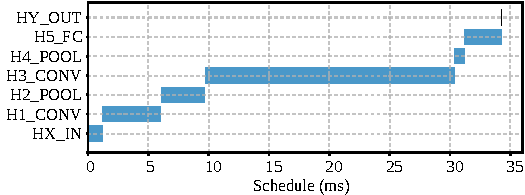
\includegraphics[width=0.5\columnwidth]{./chapters/sbs_accelerator/figures/latency_sw.pdf}
	\caption{Computation on embedded CPU.}
	\label{fig:latency_sw}
\end{figure*}

\subsubsection{Benchmark on Processing Units with Standard Floating-Point Computation}
To benchmark the computation on hardware PUs with standard floating-point, we implement the system architecture shown in \ref{fig:hw_sbs_8_pu}. In this case, the embedded software builds the SbS network as a sequential model mapping the network computation to the hardware processing units at 200 MHz as clock frequency.

\begin{figure*}[b!]
	\centering
	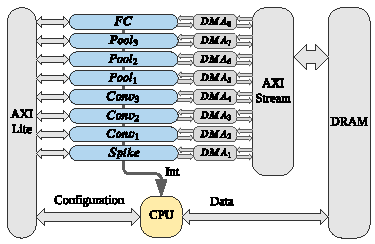
\includegraphics[width=0.5\columnwidth]{./chapters/sbs_accelerator/figures/sbs_hw_experimental.pdf}
	\caption{System overview of the top-level architecture with 8 processing units.}
	\label{fig:hw_sbs_8_pu}
\end{figure*}

The layers of the neural network with the most neurons are partitioned for asynchronous parallel processing. Since \emph{H2\_POOL} and \emph{H3\_CONV} are the layers with the most neurons, the computational workload is distributed between two PUs for each one of these layers. The output layer \emph{HY\_OUT} is fully processed by the CPU, since it is the layer with fewest neurons. The hardware mapping and the computation schedule of this deployment are displayed in \ref{tab:latency_fp} and \ref{fig:latency_pu_fp}.

\begin{table}[!t]\centering
	\caption{Performance of processing units with standard floating-point (IEEE 754) computation.}\label{tab:latency_fp}
	\scriptsize
	\begin{tabular}{llrrrrrr}\toprule
		\multicolumn{2}{c}{\textbf{Hardware mapping}} & &\multicolumn{4}{c}{\textbf{Computation schedule (ms)}} \\\cmidrule{1-2}\cmidrule{4-7}
		\textbf{Layer} &\textbf{PU} & &$t_s$ &$t_{CPU}$ &$t_{PU}$ &$t_f$ \\\midrule
		HX\_IN &Spike & &0 &0.056 &0.370 &0.426 \\
		H1\_CONV &Conv1 & &0.058 &0.598 &2.002 &2.658 \\
		\multirow{2}{*}{H2\_POOL}
		&Pool1 & &0.658 &0.126 &1.091 &1.875 \\
		&Pool2 & &0.785 &0.125 &1.075 &1.985 \\
		\multirow{2}{*}{H3\_CONV} 
		&Conv2 & &0.911 &0.280 &3.183 &4.374 \\
		&Conv3 & &1.193 &0.279 &3.176 &4.648 \\
		H4\_POOL &Pool3 & &1.473 &0.037 &0.481 &1.991 \\
		H5\_FC &FC & &1.512 &0.101 &1.118 &2.731 \\
		HY\_OUT &CPU & &1.615 &0.004 &0 &1.619 \\
		\bottomrule
	\end{tabular}
\end{table}

\begin{figure*}[b!]
	\centering
	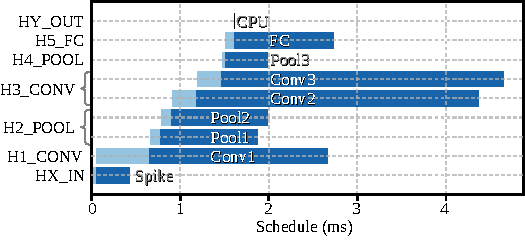
\includegraphics[width=0.5\columnwidth]{./chapters/sbs_accelerator/figures/latency_pu_fp.pdf}
	\caption{Performance of processing units with standard floating-point (IEEE 754) computation.}
	\label{fig:latency_pu_fp}
\end{figure*}

In the computation schedule, the following terms are defined as follows: $t_s(n)$ as the start time for the processing of the neural network layer (as a compute node) $n\in L$ where $L$ represents the set of layers; $t_{CPU}(n)$ as the CPU preprocessing time; $t_{PU}(n)$ as the PU latency; and $t_f(n)$ as the finish time. For data preparation, the $t_{CPU}(n)$ is the duration in which the CPU writes a DRAM buffer with $\vec{h}_\mu$ (vector of neuron latent variables) of the current processing layer and $S_t$ (input spike matrix) from its preceding layer. This buffer is streamed to the PU via DMA.

The total execution time of the CPU is defined by \ref{eq:time_cpu}. In a cyclic spiking inference, the execution time of the network computation is the longest path among the processing units including the CPU. This is denoted as the latency of an spike cycle and it is defined by \ref{eq:time_spike}. The total execution time of the network computation is the last finish time ($t_f$) in the schedule defined by \ref{eq:time_finish}.

\begin{figure*}[b!]
	\centering
	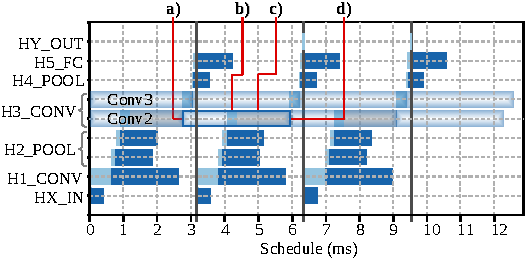
\includegraphics[width=0.5\columnwidth]{./chapters/sbs_accelerator/figures/latency_fp_cycle.pdf}
	\caption{Performance bottleneck of cyclic computation on processing units with standard floating-point (IEEE 754) arithmetic, (a) exhibits the starting of $t_{PU}$ of \emph{Conv2} on a previous computation cycle, (b) presents $t_{CPU}$ of \emph{Conv2} on the current computation cycle, (c) shows the CPU waiting time (in gray color) for \emph{Conv2} as a busy resource (awaiting for \emph{Conv2} interruption), and (d) illustrates the $t_{f}$ from the previous computation cycle, the starting of $t_{PU}$ on the current computation cycle (\emph{Conv2} interruption on completion, and start current computation cycle).}
	\label{fig:latency_pu_fp_cycle}
\end{figure*}

\begin{eqnarray} \label{eq:time_cpu}
T_{CPU} = \sum_{n\in L} t_{CPU}(n)
\end{eqnarray}

\begin{eqnarray} \label{eq:time_pu}
T_{PU} = \max_{n\in L}(t_{PU}(n))
\end{eqnarray}

\begin{eqnarray} \label{eq:time_spike}
T_{SC} =
\begin{cases}
T_{PU}, & \text{if}\ T_{CPU}\le T_{PU} \\
T_{CPU}, & \text{otherwise}
\end{cases}
\end{eqnarray}

\begin{eqnarray} \label{eq:time_finish}
T_{f} = \max_{n\in L}(t_{f}(n))
\end{eqnarray}

Using standard floating-point requires a high computational cost. As the largest layer, the computational workload of \emph{H3\_CONV} is evenly partitioned among two PUs: \emph{Conv2} and \emph{Conv3}. However, in the cyclic schedule, \emph{Conv2} causes the performance bottleneck as shown in \ref{fig:latency_pu_fp_cycle}. In this case, the CPU has to await for \emph{Conv2} to finish the computation of the previous cycle in order to start the current computation cycle. In contrast, as the smallest layer, the computational workload of \emph{HY\_OUT} is fully processed by the CPU. \ref{tab:latency_fp} and \ref{fig:latency_pu_fp} show $4\mu s$ as the processing latency of \emph{HY\_OUT}. This latency is negligible compared to the overall performance assessment. Accelerating \emph{HY\_OUT} would yield a negligible gain. Moreover, assigning a dedicated hardware PU to \emph{HY\_OUT} would add data transfer and hardware interruption handling overheads, which makes this unprofitable.

Applying \ref{eq:time_spike}, we obtain a latency of $3.18 ms$ per spike cycle. This deployment achieves an accuracy of $98.98\%$ correct classification on the $10,000$ image test set with $1000$ spikes.

The post-implementation resource utilization and power dissipation are shown in \ref{tab:resource_fp}.
%\REVIEW{The power dissipation breakdown of \emph{Conv} and \emph{FC} %are presented in {\ref{fig:power_dissipation_breakdown_float_32}}, %which exhibits data as the major component of power dissipation in %\emph{Conv}.}
Each \emph{Conv} PU instantiates an on-chip stationary weight matrix of $52,000$ entries, wish is sufficient to store $W\in\mathbb{R}^{5\times 5\times 2\times 32}$ and $W\in\mathbb{R}^{5\times 5\times 32\times 64}$ for \emph{H1\_CONV} and \emph{H3\_CONV}, respectively. In order to reduce BRAM utilization, we use a custom floating-point representation composed of 4-bit exponent and 4-bit mantissa. Each 8-bit entry is promoted to its standard floating-point representation for the dot-product computation. The methodology to find the appropriate bit-width parameters for custom floating-point representation is presented in Section~\ref{sec:parameters}.

\begin{table}[!h]\centering
	\caption{Resource utilization and power dissipation of processing units with standard floating-point (IEEE 754) computation.}\label{tab:resource_fp}
	\scriptsize
	\begin{tabular}{lrrrrrrr}\toprule
		\textbf{PU} & &\textbf{LUT} &\textbf{FF} &\textbf{DSP} &\textbf{BRAM 18K} &\textbf{Power (mW)} \\\midrule
		Spike & &2,640 &4,903 &2 &2 &38 \\
		Conv & &2,765 &4,366 &19 &37 &89 \\
		Pool & &2,273 &3,762 &5 &3 &59 \\
		FC & &2,649 &4,189 &8 &9 &66 \\
		\bottomrule
	\end{tabular}
\end{table}

%\begin{figure}[!h]
%	\centering
%	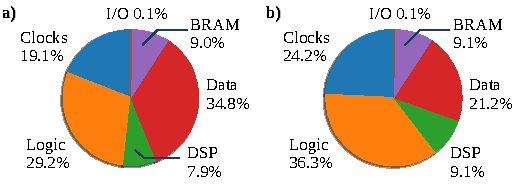
\includegraphics[width=1\columnwidth]{../figures/power_dissipation_breakdown_float-32.pdf}
%	\caption{Power dissipation breakdown of processing units with standard floating-point (IEEE 754), (a) \emph{Conv}, and (b) \emph{FC}.}
%	\label{fig:power_dissipation_breakdown_float_32}
%\end{figure}

The implementation of dot-product with standard floating-point arithmetic (IEEE 754) utilizes proprietary multiplier and adder floating-point operator cores. Vivado HLS accomplishes floating-point arithmetic operations by mapping them onto Xilinx LogiCORE IP cores, these floating-point operator cores are instantiated in the resultant RTL\cite{hrica2012floating}. In this case, the implementation of the dot-product with the standard floating-point computation reuses the multiplier and adder cores already instantiated and used in other computation sections of {\emph{Conv}} and {\emph{FC}} processing units. The post-implementation resource utilization and power dissipation of the floating-point operator cores are shown in {\ref{tab:LogiCORE}}.

\begin{table}[!h]\centering
	\caption{Resource utilization and power dissipation of multiplier and adder floating-point (IEEE 754) operator cores.}\label{tab:LogiCORE}
	\scriptsize
	\begin{tabular}{lrrrrrr}\toprule
		\textbf{Core operation} &\textbf{DSP} &\textbf{FF} &\textbf{LUT} &\textbf{Latency (clk)} &\textbf{Power (mW)} \\\midrule
		Multiplier &3 &151 &325 &4 &7 \\
		Adder &2 &324 &424 &8 &6 \\
		\bottomrule
	\end{tabular}
\end{table}

\subsubsection{Benchmark on Noise Tolerance Plot}
The noise tolerance plot serves as an intuitive visual model used to provide insights into accuracy degradation under approximate processing effects. This plot reveals inherent error resilience, and hence, approximation resilience. As an application-specific quality metric, this plot offers an effective method to estimate the overall quality degradation of the SbS network under different approximate processing effects, since both approximations and noise have qualitatively the same effect\cite{venkataramani2015approximate}.

In order to experimentally obtain the noise tolerance plot, we measure the inference accuracy of the neural network with increasing number of spikes. Then we repeat the measurements with uniformly distributed noise applied on the input images. We gradually ascend the levels of the noise amplitude, until accuracy degradation is detected. \ref{fig:accuracy_vs_noise_pu_fp} demonstrates this method using 100 sample images.

As benchmark, the tolerance plot in \ref{fig:accuracy_vs_noise_pu_fp} revels accuracy degradation having $50\%$ noise and convergence with $400$ spikes. In this case, the particular SbS network with precise processing demonstrates a remarkable inherent error resilience, hence, a great opportunity for approximate processing.


\begin{figure*}[b!]
	\centering
	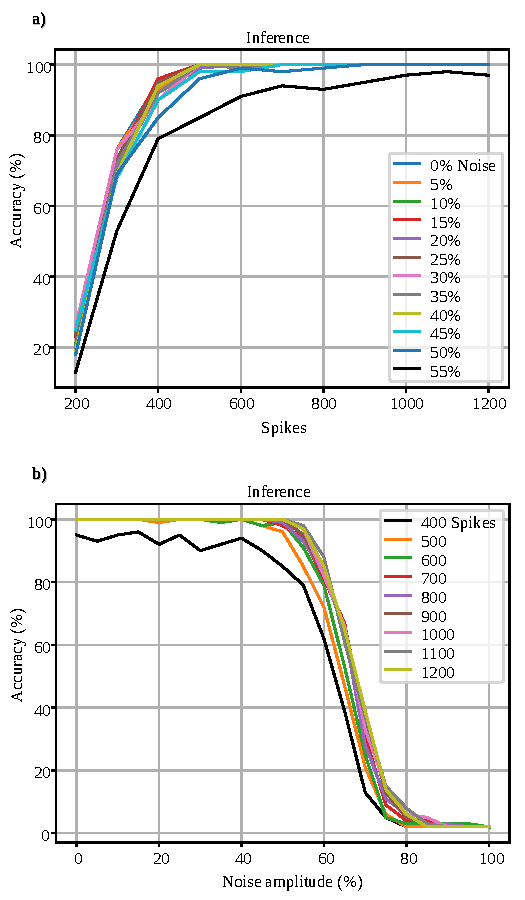
\includegraphics[width=0.5\columnwidth]{./chapters/sbs_accelerator/figures/accuracy_vs_noise_pu_fp.pdf}
	\caption{Noise tolerance on hardware PU with standard floating-point (IEEE 754) computation (benchmark/reference), (a) exhibits accuracy degradation applying $50\%$ of noise amplitude, and (b) illustrates convergence of inference with $400$ spikes.}
	\label{fig:accuracy_vs_noise_pu_fp}
\end{figure*}

\subsection{Design Exploration with Hybrid Custom Floating-Point and Logarithmic Approximation}

In this section, we address a design exploration to evaluate our approach for SbS neural network simulation using hybrid custom floating-point and logarithmic approximation. First, we examine the synaptic weight matrix of each SbS network layer in order to determine the minimum requirements for numeric representation and memory storage. Second, we implement the proposed dot-product architecture using the minimal floating-point and logarithmic representation as design parameters. Finally, we evaluate the overall performance, the inference accuracy, the resource utilization, and the power dissipation.

\subsubsection{Parameters for Numeric Representation of Synaptic Weight Matrix}
\label{sec:parameters}

	We obtain information for the numerical representation of the synaptic weight matrices from their $\log_2$-histograms presented in {\ref{fig:log2histogram}}. These histograms show the distribution of synaptic weight values in each matrix. We observe that the minimum integer exponent value is $-13$. Hence, applying {\ref{eq:exp_max}} and {\ref{eq:bits_exp}} to the given SbS network, we obtain $E_{\min}=-13$ and $N_E=4$, respectively. Therefore, 4-bits are required for the absolute binary representation of the exponents.


For quality configurability, the mantissa bit-width is a knob parameter that is tuned by the designer. This procedure leverages the builtin error-tolerance of neural networks and performs a trade-off between resource utilization and QoR. In the following subsection, we present a case study with 1-bit mantissa corresponding to the custom floating-point approximation.

\begin{figure*}[b!]
	\centering
	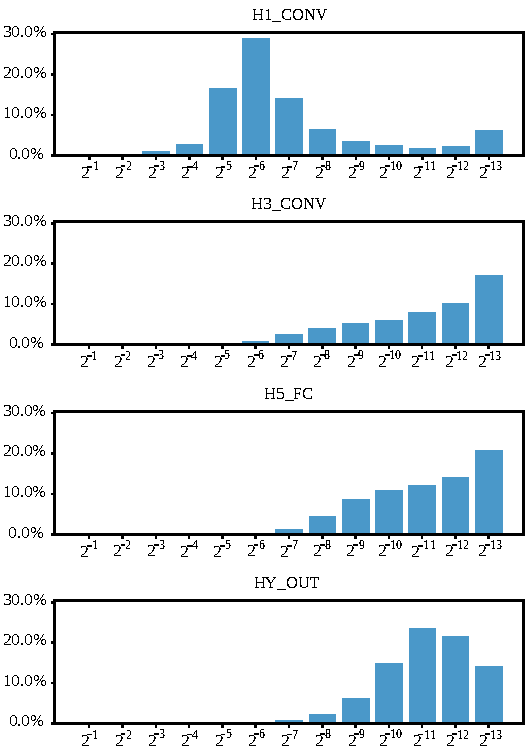
\includegraphics[width=0.5\columnwidth]{./chapters/sbs_accelerator/figures/log2_histogram.pdf}
	\caption{$\log_2$-histogram of each synaptic weight matrix showing the percentage of matrix elements with given integer exponent.}\label{fig:log2histogram}
\end{figure*}

\subsubsection{Design Exploration for Dot-product with Hybrid Custom Floating-Point Approximation}
For this design exploration, we use a custom floating-point representation composed of 4-bit exponent and 1-bit mantissa. This format is used for the synaptic weight vector on the proposed dot-product architecture. Each \emph{Conv} PU instantiates an on-chip stationary weight matrix for $52,000$ entries of 5-bit. The available memory size is large enough to store $W\in\mathbb{R}^{5\times 5\times 2\times 32}$ and $W\in\mathbb{R}^{5\times 5\times 32\times 64}$ for \emph{H1\_CONV} and \emph{H3\_CONV}, respectively. The same dot-product architecture is implemented in the processing unit of the fully connected layer (\emph{FC}). However, due to lack of BRAM resources, this PU can not instantiate on-chip stationary synaptic weight matrix. Instead, \emph{FC} receives the $\vec{W}(s_t)$ (weight vectors) during operation as well as $\vec{h}_\mu$ and $S_t$. The hardware mapping and the computation schedule of this implementation are displayed in \ref{tab:latency_cfp} and \ref{fig:latency_pu_cfp_cycle}.

As shown in the computation schedule in \ref{tab:latency_cfp} and \ref{fig:latency_pu_cfp_cycle}, this implementation achieves a maximum hardware PU latency of $1.30 ms$ according to \ref{eq:time_pu}, and a CPU latency of $1.67 ms$. Therefore, applying \ref{eq:time_spike}, we obtain a latency of $1.67 ms$ per spike cycle as shown in \ref{fig:latency_pu_cfp_cycle}. In this case, the cyclic bottleneck is in the performance of the CPU.

This configuration achieves an accuracy of $98.97\%$ correct classification on the $10,000$ image test set with $1000$ spikes. This indicates an accuracy degradation of $0.33\%$. For output quality monitoring, the noise tolerance plot in \ref{fig:accuracy_vs_noise_pu_cfp} revels accuracy degradation for noise higher than $50\%$ on the input images, and convergence of inference with $400$ spikes. Thus, the particular SbS network implementation under approximate processing effects demonstrates a minimal impact on the overall accuracy. This proves an inherent error resilience, and hence, remaining approximation budget.

The post-implementation resource utilization and power dissipation
%\REVIEW{breakdown}
are shown in \ref{tab:resource_cfp}
%\REVIEW{and {\ref{fig:power_dissipation_breakdown_float_5}}, respectively}
.

\begin{table}[h!]\centering
	\caption{Resource utilization and power dissipation of processing units with hybrid custom floating-point approximation.}\label{tab:resource_cfp}
	\scriptsize
	\begin{tabular}{lrrrrrrr}\toprule
		\textbf{PU} & &\textbf{LUT} &\textbf{FF} &\textbf{DSP} &\textbf{BRAM 18K} &\textbf{Power (mW)} \\\midrule
		Conv & &3,139 &4,850 &19 &25 &82 \\
		FC & &3,265 &5,188 &8 &9 &66 \\
		\bottomrule
	\end{tabular}
\end{table}

%\begin{figure}[!h]
%	\centering
%	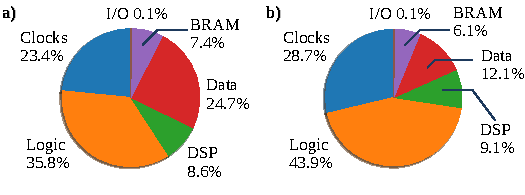
\includegraphics[width=1\columnwidth]{../figures/power_dissipation_breakdown_float-5.pdf}
%	\caption{Power dissipation breakdown of processing units with hybrid custom floating-point approximation, (a) \emph{Conv}, and (b) \emph{FC}.}
%	\label{fig:power_dissipation_breakdown_float_5}
%\end{figure}


\begin{table}[t!]\centering
	\caption{Performance of hardware processing units with hybrid custom floating-point approximation.}\label{tab:latency_cfp}
	\scriptsize
	\begin{tabular}{llrrrrrr}\toprule
		\multicolumn{2}{c}{\textbf{Hardware mapping}} & &\multicolumn{4}{c}{\textbf{Computation schedule (ms)}} \\\cmidrule{1-2}\cmidrule{4-7}
		\textbf{Layer} &\textbf{PU} & &$t_s$ &$t_{CPU}$ &$t_{PU}$ &$t_f$ \\\midrule
		HX\_IN &Spike & &0 &0.055 &0.307 &0.362 \\
		H1\_CONV &Conv1 & &0.057 &0.654 &1.309 &2.020 \\
		\multirow{2}{*}{H2\_POOL} &Pool1 & &0.713 &0.131 &1.098 &1.942 \\
		&Pool2 & &0.845 &0.125 &1.098 &2.068 \\
		\multirow{2}{*}{H3\_CONV} &Conv2 & &0.972 &0.285 &1.199 &2.456 \\
		&Conv3 & &1.258 &0.279 &1.184 &2.721 \\
		H4\_POOL &Pool3 & &1.538 &0.037 &0.484 &2.059 \\
		H5\_FC &FC & &1.577 &0.091 &0.438 &2.106 \\
		HY\_OUT &CPU & &1.669 &0.004 &0 &1.673 \\
		\bottomrule
	\end{tabular}
\end{table}

\begin{figure*}[b!]
	\centering
	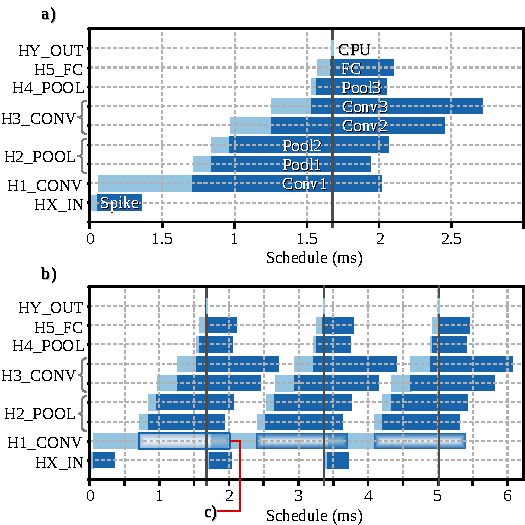
\includegraphics[width=0.5\columnwidth]{./chapters/sbs_accelerator/figures/latency_cfp_cycle.pdf}
	\caption{Performance on processing units with hybrid custom floating-point approximation, (a) exhibits computation schedule, (b) presents cyclic computation schedule, and (c) shows the performance of \emph{Conv2} from a previous computation cycle during the preprocessing of \emph{H1\_CONV} on the current computation cycle without bottleneck.}
	\label{fig:latency_pu_cfp_cycle}
\end{figure*}

\begin{figure*}[b!]
	\centering
	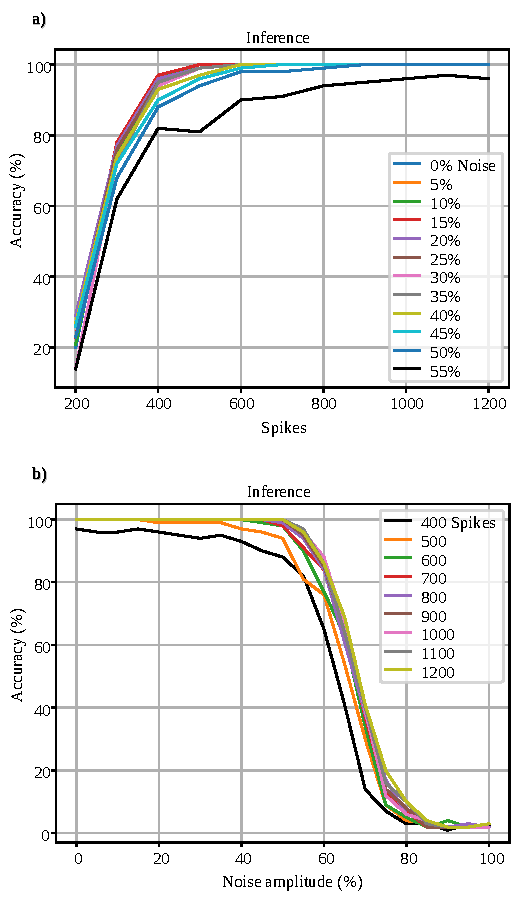
\includegraphics[width=0.5\columnwidth]{./chapters/sbs_accelerator/figures/accuracy_vs_noise_pu_cfp(4-bit-exponent_1-bit-mantissa).pdf}
	\caption{Noise tolerance on hardware PU with custom floating-point approximation, (a) exhibits accuracy degradation applying $50\%$ of noise amplitude, and (b) illustrates convergence of inference with $400$ spikes.}
	\label{fig:accuracy_vs_noise_pu_cfp}
\end{figure*}

\subsubsection{Design Exploration for Dot-Product whit Hybrid Logarithmic Approximation}
As the most efficient setup and yet the worst-case quality configuration, we use a 4-bit integer exponent for logarithmic representation of the synaptic weight matrix. Each \emph{Conv} processing unit implements the proposed dot-product architecture including an on-chip stationary weight matrix for $52,000$ entries of 4-bit integer each one to store $W\in\mathbb{N}^{5\times 5\times 2\times 32}$ and $W\in\mathbb{N}^{5\times 5\times 32\times 64}$ for \emph{H1\_CONV} and \emph{H3\_CONV}, respectively. The same dot-product architecture is implemented in the \emph{FC} processing unit without stationary synaptic weight matrix. The hardware mapping and the computation schedule of this implementation are displayed in \ref{tab:latency_log} and \ref{fig:latency_pu_log_cycle}.

As shown in the computation schedule in \ref{tab:latency_log} and \ref{fig:latency_pu_log_cycle}, this implementation achieves a maximum hardware PU latency of $1.27 ms$ according to \ref{eq:time_pu}, and a CPU latency of $1.67 ms$. Therefore, applying \ref{eq:time_spike}, we obtain a latency of $1.67 ms$ per spike cycle as shown in \ref{fig:latency_pu_log_cycle}. In this case, the cyclic bottleneck is in the CPU performance.

This quality configuration achieves an accuracy of $98.84\%$ correct classification on the $10,000$ image test set with $1000$ spikes. This indicates an accuracy degradation of $0.46\%$. For output quality monitoring, the noise tolerance plot in \ref{fig:accuracy_vs_noise_pu_log} revels accuracy degradation having $40\%$ noise on the input images, and convergence of inference with $600$ spikes. The particular SbS network implementation under approximate processing demonstrates a minor impact on the overall accuracy. This exhibits remaining budget for further approximate processing approaches.

The post-implementation resource utilization and power dissipation
%\REVIEW{breakdown}
are shown in \ref{tab:resource_log}
%\REVIEW{and {\ref{fig:power_dissipation_breakdown_log_4}}, respectively}
.

\begin{table}[t!]\centering
	\caption{Performance of hardware processing units with hybrid logarithmic approximation.}\label{tab:latency_log}
	\scriptsize
	\begin{tabular}{llrrrrrr}\toprule
		\multicolumn{2}{c}{\textbf{Hardware mapping}} & &\multicolumn{4}{c}{\textbf{Computation schedule (ms)}} \\\cmidrule{1-2}\cmidrule{4-7}
		\textbf{Layer} &\textbf{PU} & &$t_s$ &$t_{CPU}$ &$t_{PU}$ &$t_f$ \\\midrule
		HX\_IN &Spike & &0 &0.055 &0.264 &0.319 \\
		H1\_CONV &Conv1 & &0.057 &0.655 &1.271 &1.983 \\
		\multirow{2}{*}{H2\_POOL} &Pool1 & &0.714 &0.130 &1.074 &1.918 \\
		&Pool2 & &0.845 &0.126 &1.106 &2.077 \\
		\multirow{2}{*}{H3\_CONV} &Conv2 & &0.973 &0.285 &1.179 &2.437 \\
		&Conv3 & &1.258 &0.278 &1.176 &2.712 \\
		H4\_POOL &Pool3 & &1.538 &0.037 &0.488 &2.063 \\
		H5\_FC &FC & &1.577 &0.091 &0.388 &2.056 \\
		HY\_OUT &CPU & &1.669 &0.004 &0 &1.673 \\
		\bottomrule
	\end{tabular}
\end{table}

\begin{figure*}[b!]
	\centering
	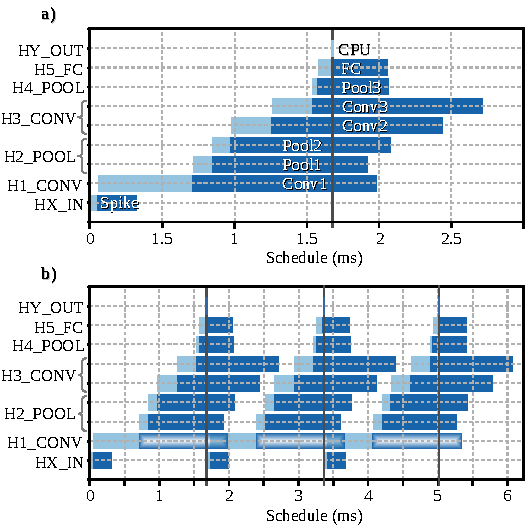
\includegraphics[width=0.5\columnwidth]{./chapters/sbs_accelerator/figures/latency_log_cycle.pdf}
	\caption{Performance of processing units with hybrid logarithmic approximation, (a) exhibits computation schedule, and (b) illustrates cyclic computation schedule.}
	\label{fig:latency_pu_log_cycle}
\end{figure*}

\begin{table}[!h]\centering
	\caption{Resource utilization and power dissipation of processing units with hybrid logarithmic approximation.}\label{tab:resource_log}
	\scriptsize
\begin{tabular}{lrrrrrrr}\toprule
	\textbf{PU} & &\textbf{LUT} &\textbf{FF} &\textbf{DSP} &\textbf{BRAM 18K} &\textbf{Power (mW)} \\\midrule
	Conv & &3,086 &4,804 &19 &21 &78 \\
	FC & &3,046 &4,873 &8 &8 &66 \\
	\bottomrule
\end{tabular}
\end{table}

%\begin{figure}[!h]
%	\centering
%	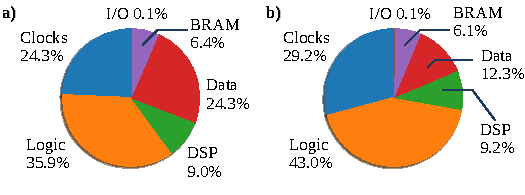
\includegraphics[width=1\columnwidth]{../figures/power_dissipation_breakdown_log-4.pdf}
%	\caption{Power dissipation breakdown of processing units with hybrid logarithmic approximation, (a) \emph{Conv}, and (b) \emph{FC}.}
%	\label{fig:power_dissipation_breakdown_log_4}
%\end{figure}



\begin{figure*}[b!]
	\centering
	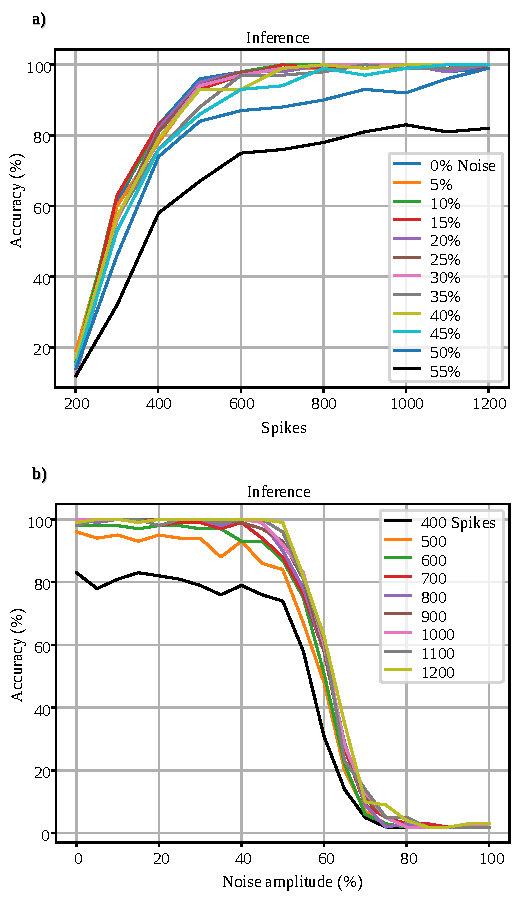
\includegraphics[width=0.5\columnwidth]{./chapters/sbs_accelerator/figures/accuracy_vs_noise_pu_log.pdf}
	\caption{Noise tolerance on hardware PU with hybrid logarithmic approximation, (a) exhibits accuracy degradation applying $40\%$ of noise amplitude, (b) illustrates convergence of inference with $600$ spikes.}
	\label{fig:accuracy_vs_noise_pu_log}
\end{figure*}


\subsection{Results and Discussion}
As a reference, the SbS network simulation on embedded CPU using standard 32-bit floating-point achieves an accuracy of $99.3\%$ with a latency of $T_{SC} = 34.28ms$. As a second reference point, the network simulation on hardware processing units with standard floating-point achieves an accuracy of $98.98\%$ with a latency $T_{SC}=3.18ms$. As result we get a $10.7\times$ latency enhancement and an accuracy degradation of $0.32\%$. The tolerance plot in \ref{fig:accuracy_vs_noise_pu_fp} reveals accuracy degradation having $50\%$ noise on the input images, and convergence of inference with $400$ spikes. In this case, the SbS network deployment with precise computing proves extraordinary inherent error resilience, and hence, this represents a great potential for approximate processing.

As a demonstration of the proposed dot-product architecture, the SbS network simulation on hardware PUs with synaptic representation using 5-bit custom floating-point (4-bit exponent, 1-bit mantissa) and 4-bit logarithmic (4-bit exponent) achieve $20.5\times$ latency enhancement and accuracy of $98.97\%$ and $98.84\%$, respectively. This results in an accuracy degradation of $0.33\%$ and $0.46\%$, respectively. For output quality monitoring, the noise tolerance plot in \ref{fig:accuracy_vs_noise_pu_cfp} and \ref{fig:accuracy_vs_noise_pu_log} reveal accuracy degradation when having $50\%$ and $40\%$ noise on the input images, and convergence of inference with $400$ and $600$ spikes, respectively. Therefore, the design exploration under the proposed approximate computing approach indicates sufficient inherent error resilience for further and more aggressive approximate processing approaches.

Regarding resource utilization and power dissipation with the proposed approach, the \emph{Conv} processing units have a $43.24\%$ reduction of BRAM, and a $12.35\%$ of improvement in energy efficiency over the standard floating-point implementation. However, the proposed approach does not reuse the available floating-point operator cores instantiated from other computational sections (see {\ref{tab:LogiCORE}}). Therefore, the logic required for the dot-product must be implemented, which is reflected as additional utilization of LUT and FF resources. The experimental results of the design exploration are summarized in \ref{tab:results}. The platform implementations are summarized in \ref{tab:platform_comparison}, and their power dissipation breakdowns are presented in {\ref{fig:platform_power_dissipation_breakdown}}.

\begin{table*}[!t]
	\begin{threeparttable}
		\centering
		\caption{Experimental results.}\label{tab:results}
		\scriptsize
		\begin{tabular}{lrrrrrrrrrrrrrr}\toprule
			\multirow{2}{*}{\textbf{Dot-product implementation}} &\multirow{2}{*}{\textbf{PU}} &\multicolumn{4}{c}{\textbf{Post-implementation resource utilization}} & &\multirow{2}{*}{\textbf{Power (mW)}} & &\multicolumn{2}{c}{\textbf{Latency}} & &\multicolumn{2}{c}{\textbf{Accuracy (\%)\tnote{e}}} \\\cmidrule{3-6}\cmidrule{10-11}\cmidrule{13-14}
			& &\textbf{LUT} &\textbf{FF} &\textbf{DSP} &\textbf{BRAM 18K} & & & &$T_{SC}$ \textbf{(ms)} &\textbf{Gain\tnote{d}} & &\textbf{Noise 0\%} &\textbf{50\%} \\\midrule
			\multirow{2}{*}{Standard floating-point computation\tnote{a}} &Conv &2,765 &4,366 &19 &37 & &89 & &\multirow{2}{*}{3.18} &\multirow{2}{*}{10.7x} & &\multirow{2}{*}{98.98} &\multirow{2}{*}{98.63} \\
			&FC &2,649 &4,189 &8 &9 & &66 & & & & & & \\
			& & & & & & & & & & & & & \\
			\multirow{2}{*}{Hybrid custom floating-point approx\tnote{b}} &Conv &3,139 &4,850 &19 &25 & &82 & &\multirow{2}{*}{1.67} &\multirow{2}{*}{20.5x} & &\multirow{2}{*}{98.97} &\multirow{2}{*}{98.47} \\
			&FC &3,265 &5,188 &8 &9 & &66 & & & & & & \\
			& & & & & & & & & & & & & \\
			\multirow{2}{*}{Hybrid logarithmic approximation\tnote{c}} &Conv &3,086 &4,804 &19 &21 & &78 & &\multirow{2}{*}{1.67} &\multirow{2}{*}{20.5x} & &\multirow{2}{*}{98.84} &\multirow{2}{*}{95.22} \\
			&FC &3,046 &4,873 &8 &8 & &66 & & & & & & \\
			\bottomrule
		\end{tabular}
		\begin{tablenotes}
			\scriptsize
			\item[a] Reference with standard floating-point arithmetic (IEEE 754).
			\item[b] Synaptic weight with number representation composed of 4-bit exponent and 1-bit mantissa.
			\item[c] Synaptic weight with number representation composed of 4-bit exponent.
			\item[d] Acceleration with respect to the computation on embedded CPU (ARM Cortex-A9 at 666 MHz) with latency $T_{SC} = 34.28 ms$.
			\item[e] Accuracy on 10,000 image test set with 1000 spikes.
		\end{tablenotes}
	\end{threeparttable}
\end{table*}

\begin{table*}[!t]
	\begin{threeparttable}
		\centering
		\caption{Platform implementations.}\label{tab:platform_comparison}
		\scriptsize
		\begin{tabular}{lrrrrrrrrrr}\toprule
			\multirow{2}{*}{\textbf{Platform implementation}} &\multicolumn{4}{c}{\textbf{Post-implementation resource utilization}} &\multirow{2}{*}{\textbf{Power (W)}} &\multirow{2}{*}{\textbf{Clock (MHz)}} &\multicolumn{2}{c}{\textbf{Latency}} &\multirow{2}{*}{\textbf{Accuracy (\%)\tnote{f}}} \\\cmidrule{2-5}\cmidrule{8-9}
			&\textbf{LUT} &\textbf{FF} &\textbf{DSP} &\textbf{BRAM 18K} & & &$T_{SC}$ \textbf{(ms)} &\textbf{Gain\tnote{e}} & \\\midrule
			\ref{nevarez2020accelerator}\tnote{a} &42,740 &57,118 &49 &92 &2.519 &250 &4.65 &7.4x &99.02 \\
			This work (standard floating-point computation)\tnote{b} &39,514 &56,036 &82 &180 &2.420 &200 &3.18 &10.7x &98.98 \\
			This work (hybrid custom floating-point approx)\tnote{c} &42,021 &58,759 &82 &156 &2.369 &200 &1.67 &20.5x &98.97 \\
			This work (hybrid logarithmic approximation)\tnote{d} &41,060 &57,862 &82 &148 &2.324 &200 &1.67 &20.5x &98.84 \\
			\bottomrule
		\end{tabular}
		\begin{tablenotes}
			\scriptsize
			\item[a] Reference architecture with homogeneous AUs using standard floating-point arithmetic (IEEE 754).
			\item[b] Reference architecture with specialized heterogeneous PUs using standard floating-point arithmetic (IEEE 754).
			\item[c] Proposed architecture with specialized heterogeneous PUs using synaptic weight with number representation composed of 4-bit exponent and 1-bit mantissa.
			\item[d] Proposed architecture with specialized heterogeneous PUs using synaptic weight with number representation composed of 4-bit exponent.
			\item[e] Acceleration with respect to the computation on embedded CPU (ARM Cortex-A9 at 666 MHz) with latency $T_{SC} = 34.28 ms$.
			\item[f] Accuracy on 10,000 image test set with 1000 spikes.
		\end{tablenotes}
	\end{threeparttable}
\end{table*}

\begin{figure*}[b!]
	\centering
	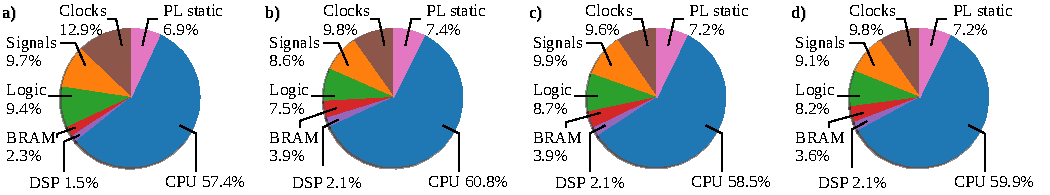
\includegraphics[width=\columnwidth]{./chapters/sbs_accelerator/figures/platform_power_dissipation_breakdown.pdf}
	\caption{Power dissipation breakdown of platform implementations, (a) \ref{nevarez2020accelerator} architecture with homogeneous AUs using standard floating-point arithmetic (IEEE 754), (b) reference architecture with specialized heterogeneous PUs using standard floating-point arithmetic (IEEE 754), (c) proposed architecture with hybrid custom floating-point approximation, and (d) proposed architecture with hybrid logarithmic approximation.}
	\label{fig:platform_power_dissipation_breakdown}
\end{figure*}
\section{Conclusions}
\label{sec:conclusions}
In this work, we accelerate SbS neural networks with a dot-product functional unit based on approximate computing that combinesthe advantages of custom floating-point and logarithmic representations. This approach reduces computational latency, memory footprint, and power dissipation while preserving classification accuracy. For output quality monitoring, we applied noise tolerance plots as an intuitive visual measure to provide insights into the accuracy degradation of SbS networks under different approximate processing effects. This plot revels inherent error resilience, hence, the possibilities for approximate processing.


We demonstrate our approach using a design exploration flow on a Xilinx Zynq-7020 with a deployment of SbS network for the MNIST classification task. This implementation achieves up to $20.5\times$ latency enhancement, $8\times$ weight memory footprint reduction, and $12.35\%$ of energy efficiency improvement over the standard floating-point hardware implementation, and incurs in less than $0.5\%$ of accuracy degradation. Furthermore, with a noise amplitude of $50\%$ added on top of the input images, the SbS network presents an accuracy degradation of less than $5\%$. As output quality monitor, the resulting noise tolerance plots demonstrate a sufficient QoR for minimal impact on the overall accuracy of the neural network under the effects of the proposed approximation technique. These results suggest available room for further and more aggressive approximate processing approaches.


In summary, based on the relaxed need for fully accurate or deterministic computation of SbS neural networks, approximate computing techniques allow substantial enhancement in processing efficiency with moderated accuracy degradation.

\chapter{Accelerating Convolutional Neural Networks}\label{chap.cnn}
\minitoc

\section{Introduction}
\label{sec:introduction}
%%% General intro
There is a growing demand for ubiquitous AI sensor analytics. Industry 4.0 and smart city infrastructure leverage AI solutions to increase productivity and adaptability\cite{lom2016industry}. These solutions are powered by advances in ML, compute engines, and big data. Hence, improvements of these should be considered for research, as they are the machinery of the future.

Convolutional neural networks (CNNs) represent the essential building blocks in 2D pattern analytics. Sensor-based applications such as mechanical fault diagnosis\cite{li2019sensor,dong2018rolling}, structural health monitoring\cite{nagayama2007structural}, human activity recognition (HAR) \cite{wang2019deep}, hazardous gas detection\cite{kim2017hazardous} have been powered by CNN models in industry and academia. CNN-based models, as one of the main types of artificial neural networks (ANNs), have been widely used in sensor analytics with automatic learning from sensor data \cite{ince2016real, janssens2016convolutional, abdeljaber2017real, guo2016hierarchical}. In this context, CNN models are applied for automatic feature learning, usually, from 1D time series as well as for 2D time-frequency spectrograms. CNN models provide advantages such as local dependency, scale invariance, and noise resilience in analytics\cite{du2014leveraging}. However, these models are computationally intensive and power-hungry. This is particularly challenging for low-power embedded applications in the field of Internet-of-Things (IoT).

For ML inference, dedicated hardware architectures are typically used to enhance compute performance and power efficiency. In terms of computational throughput, graphics processing units (GPUs) offer the highest performance; in terms of power efficiency, ASIC and FPGA solutions are more energy efficient \cite{nurvitadhi2017can}. As a result, numerous commercial ASIC and FPGA accelerators have been proposed, targeting both high performance computing (HPC) for data-centers and embedded systems applications.

However, most FPGA accelerators have been implemented to target mid- to high-range FPGAs for computationally intensive CNN models such as AlexNet, VGG-16, and ResNet-18. The main drawbacks of these implementations are power supply demands, physical dimensions, heat sink requirements, air cooling, and a resulting high price. In some cases, these implementations are not feasible for ubiquitous low-power/resource-constrained applications.

To reduce the compute hardware for CNN inference there are two types of research \cite{wu2021low}: the first one is deep compression including weight pruning, weight quantization, and compression storage \cite{han2015deep,han2015learning}; the second type of research corresponds to a more efficient data representation, also known as custom quantization for dedicated hardware implementation. In this group, hardware implementations with customized 8-bit floating-point computation have been proposed \cite{mei2017200mhz, wu2021low, lian2019high}. However, these architectures are inadequate for embedded applications, the target devices are high-end FPGA and PCIe devices.

Reducing the compute hardware with more aggressive quantization such as binary \cite{courbariaux2015binaryconnect}, ternary \cite{lin2015neural}, and mixed precision (2-bit activations and ternary weights) \cite{colangelo2018exploration} typically incur significant accuracy degradation for very low precisions, especially for complex problems\cite{faraone2019addnet}.

In this paper, we present the Hybrid-Float6 quantization and its dedicated hardware design. In this concept, feature maps are represented by standard 32-bit FP and trainable parameters by 6-bit FP. To preserve accuracy, we introduce a quantization-aware training (QAT) method. To preserve model accuracy, we present a quantization-aware training method, which in some cases improves model performance. For ML compatibility/portability, the 6-bit FP is wrapped into the standard FP representation. The dedicated hardware design extracts the 6-bit format automatically and performs the computation. We propose a parameterized tensor processor implementing a pipelined vector dot-product with HF6. The 6-bit FP representation uses 4-bit exponent and 1-bit mantissa. This approach enables an optimized MAC design by reducing the mantissa multiplication to a mux-adder operation. We leverage the intrinsic error tolerance of ANN to further reduce the hardware design with approximation. This approach reduces latency, resource utilization, and power dissipation. The embedded hardware/software architecture is integrated with TensorFlow Lite using delegate interface to accelerate \emph{Conv2D} tensor operations. We evaluate the applicability of our approach with a CNN-regression model and hardware design exploration for sensor analytics of SHM for anomaly localization. The embedded hardware/software framework is demonstrated on XC7Z007S as the smallest and most inexpensive Zynq SoC device, see \Fig{fig:workflow}. To the best of our knowledge, this is the first research addressing 6-bit floating-point quantization on CNN models and its dedicated hardware design.

\begin{figure*}[b!]
	\centering
	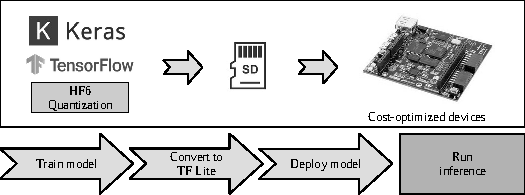
\includegraphics[width=0.5\columnwidth]{./chapters/cnn_accelerator/figures/workflow.pdf}
	\caption{The workflow of our approach on embedded FPGAs.}
	\label{fig:workflow}
\end{figure*}

Our main contributions are as follows:
\begin{enumerate}
	\item
	
	We present the Hybrid-Float6 quantization and its dedicated hardware design. We propose an optimized hardware MAC by reducing the mantissa multiplication to a mux-adder operation. We exploit the intrinsic error tolerance of ANN to further reduce the hardware design with approximation. To preserve model accuracy, we present a quantization-aware training method, which in some cases improves accuracy.
	
	\item We develop a custom hardware/software co-design framework for sensor analytics applications on low-power embedded FPGAs. This architecture integrates TensorFlow Lite.
	\item We present a customizable tensor processor as a dedicated hardware for HF6. This design computes \emph{Conv2D} tensor operations employing a pipelined vector dot-product with parametrized on-chip memory utilization. The compute engine can be implemented with standard floating-point (with FP Xilinx LogiCORE IPs) and HF6.
	\item We demonstrate the potential of our approach with a CNN-regression model for anomaly localization in SHM based on AE. We address a hardware design exploration. We evaluate inference accuracy, compute performance, hardware resource utilization, and energy consumption.
\end{enumerate}

The rest of the paper is organized as follows. Section~\ref{sec:related_work} covers the related work; Section~\ref{sec:background} introduces the background for \emph{Conv2D} tensor operation and floating-point number representation; Section~\ref{sec:system_design} describes the system design of the hardware/software architecture and the quantized aware training method; Section~\ref{sec:experimental_results} presents the experimental results thorough a design exploration flow; Section~\ref{sec:conclusions} concludes the paper.

This work is available to the community as an open-source project at https://github.com/YaribNevarez/tensorflow-lite-fpga-delegate.git.
\section{Related work}
\label{sec:related_work}
In the literature we find plenty of hardware architectures for CNN accelerators implemented in \gls{fpga}. Most of the research work implements fixed-point quantization, and very limited research focuses on \gls{fp}. Moreover, to the best of my knowledge, there is no research work related to \gls{fp} inference for low-power embedded applications.


\subsection{Hybrid Custom Floating-Point}
In \cite{lai2017deep}, Liangzhen Lai et al. proposed a mixed data representation with floating-point for weights and fixed-point for activations. This work demonstrated on SqueezeNet, AlexNet, GoogLeNet, and VGG-16 that 8-bit floating-point quantization (4-bit exponent and 3-bit mantissa) results in constant negligible accuracy degradation. Similarly, in \cite{settle2018quantizing}, Sean O. Settle et al. presented an 8-bit \gls{fp} quantization scheme, which needs an extra inference batch to compensate for quantization errors. However, \cite{lai2017deep} and \cite{settle2018quantizing} did not present a dedicated hardware architecture.

In \cite{lian2019high}, Xiaocong Lian et al. proposed a hardware accelerator with optimized block floating-point (BFP). In this design the activations and weights are represented by 16-bit and 8-bit \gls{fp} formats, respectively. This design is demonstrated on Xilinx VC709 evaluation board. This implementation achieves throughput and power efficiency of \unit[760.83]{GOP/s} and \unit[82.88]{GOP/s/W}, respectively. However, this design is not suitable for low-power resource-constrained embedded \glspl{fpga}.

\subsection{Low-Precision Floating-Point}
In \cite{mei2017200mhz}, Chunsheng Mei et al. presented a hardware accelerator for VGG16 model using half-precision \gls{fp} (16-bit). This design is demonstrated on Xilinx Virtex-7 (XC7VX690T) with PCIe interface. This implementation achieves throughput and power efficiency of \unit[202.8]{GFLOP/s} and \unit[18.72]{GFLOP/s/W}, respectively. In \cite{wu2021low}, Chen Wu et al. proposed a low-precision (8-bit) floating-point (LPFP) quantization method for \gls{fpga}-based acceleration. This design is demonstrated on Xilinx Kintex 7 and Ultrascale/Ultrascale+. This implementation achieves throughput and power efficiency of \unit[1086.8]{GOP/s} and \unit[115.4]{GOP/s/W}, respectively.

\subsection{Low-Power}
Two research papers have been reported hardware accelerators targeting XC7Z007S. This is the smallest and most inexpensive device from Zynq-7000 SoC family. In \cite{meloni2019cnn}, Paolo Meloni et al. presented a \gls{cnn} inference accelerator for compact and cost-optimized devices. This implementation uses fixed-point to process light-weight \gls{cnn} architectures with a power efficiency between \unit[2.49] to \unit[2.98]{GOPS/s/W}. In \cite{gao2020edgedrnn}, Chang Gao et al. presented EdgeDRNN, a \gls{rnn} accelerator for edge inference. This implementation adopts the \gls{snn} inspired delta network algorithm to exploit temporal sparsity in \glspl{rnn}.
\section{System Design}
\label{sec:system_design}
The system design is a hardware/software co-design framework for low-power AI deployment. This architecture allows design exploration of dedicated hardware integrated with TensorFlow Lite on low-cost embedded FPGAs.

\subsection{Base Embedded System Architecture}
The base embedded system architecture implements a cooperative hardware-software platform. See \Fig{fig:system_architecture}. The embedded CPU delegates low-level compute-bound tensor operations to the TPs. The TPs employ AXI-Lite interface for configuration and AXI-Stream interfaces via Direct Memory Access (DMA) for data movement from DDR memory. Each TP asserts an interrupt flag once the job/transaction is complete. Interrupt events are handled by the embedded CPU to collect results and start a new transaction. The hardware architecture can vary its resource utilization by customizing the TPs prior to the hardware synthesis.
\begin{figure*}[b!]
	\centering
	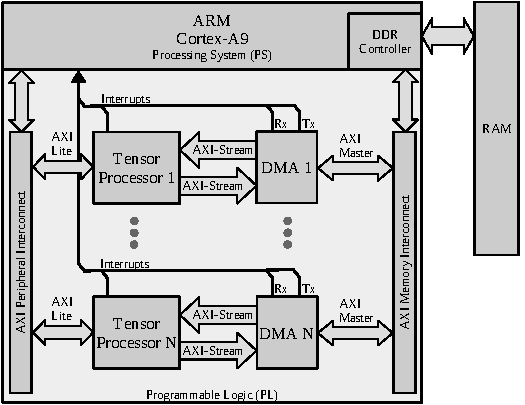
\includegraphics[width=0.5\columnwidth]{./chapters/cnn_accelerator/figures/system_design.pdf}
	\caption{Base embedded system architecture.}
	\label{fig:system_architecture}
\end{figure*}
\subsection{Tensor Processor}
The TP is a dedicated hardware module to compute tensor operations. This architecture implements high performance communication with AXI-Stream, direct CPU communication with AXI-Lite, and on-chip storage utilizing BRAM. This hardware architecture is implemented with high-level synthesis (HLS). The tensor operations are implemented based on the C++ TensorFlow Lite micro kernels. See \fig{fig:accelerator}.

The TP is an extensible hardware module that executes low-level tensor operations. In this paper, we focus on the \emph{Conv2D} tensor operation that computes 2D convolution layers.

\begin{figure*}[b!]
	\centering
	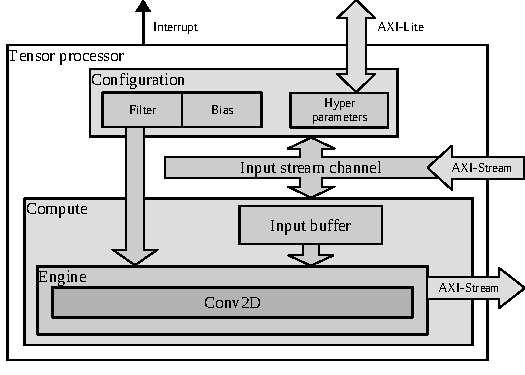
\includegraphics[width=0.5\columnwidth]{./chapters/cnn_accelerator/figures/accelerator.pdf}
	\caption{Hardware architecture of the proposed tensor processor.}
	\label{fig:accelerator}
\end{figure*}
\subsubsection{Modes of Operation}
The TP has two modes of operation: \emph{configuration} and \emph{execution}.
\begin{itemize}
	\item In \emph{configuration} mode, the TP receives the tensor operation hyperparameters: stride, dilation, padding, offset, activation, depth-multiplier, input shape, filter shape, bias shape, and output shape. Afterwards, the TP receives filter and bias tensors, which are locally stored in BRAM. The filter and bias tensors are transferred with standard FP representation. Then, the TP extracts the 6-bit FP format for local on-chip storage.
	
	\item In \emph{execution} mode, the TP executes the tensor operation according to the hyperparameters given in the configuration mode. During execution, the input and output tensors are moved from/to the off-chip memory via DMA.
\end{itemize}
\subsubsection{Dot-Product with Hybrid Floating-Point Computation}
\label{sec:dot_product}
We implement the floating-point computation adopting the dot-product with hybrid custom floating-point\cite{nevarez2021accelerating}. The hardware dot-product is illustrated in \Fig{fig:dot_product} and \Fig{fig:dot_product_loop}(a). This design instantiates an HF6 MAC and an accumulator variable of 64-bit fixed-point with 23-bit fraction. During operation, the feature map and filter values are extracted from on-chip memory (BRAM). Both values have to be different than zero to enable the MAC operation. The result is biased by accumulating a denormalized bias value. Since the bias is stored with 6-bit FP, its fractional part has to be aligned with the 23-bit fraction of the accumulator, see \Fig{fig:dot_product_loop}(b). The ReLu activation is applied and the result is normalized to converted to IEEE 754 standard FP, see \Fig{fig:dot_product_loop}(c).

Rather than a parallelized structure, this is a pipelined hardware design suitable for resource-limited devices. The latency in clock cycles of this hardware module is defined by \equ{eq:dot_custom_float_latency}, where $N$ is the vector length. This latency equation is obtained from the general pipelined hardware latency formula: $L=\left(N-1\right)II+IL$, where $II$ is the initiation interval, and $IL$ is the iteration latency. Both $II$ and $IL$ are obtained from the high-level synthesis results. Both the exponent and mantissa bit widths of the filter and bias buffers are set to a 4-bit exponent and a 1-bit mantissa (E4M1), which corresponds to float6 quantization.

\begin{eqnarray} \label{eq:dot_custom_float_latency}
L_{hf}=N+7
\end{eqnarray}

\begin{figure*}[b!]
	\centering
	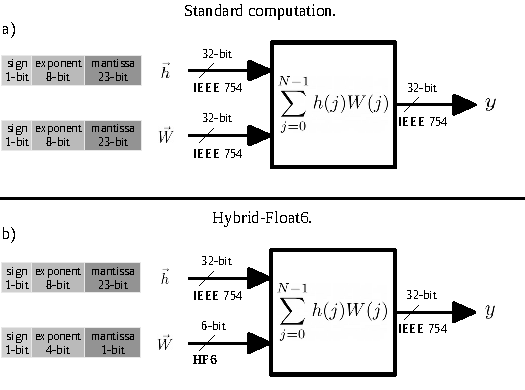
\includegraphics[width=0.5\columnwidth]{./chapters/cnn_accelerator/figures/dot-product_unit.pdf}
	\caption{Dot-product hardware module with (a) standard floating-point and (b) Hybrid-Float6.}
	\label{fig:dot_product}
\end{figure*}

\begin{figure*}[b!]
	\centering
	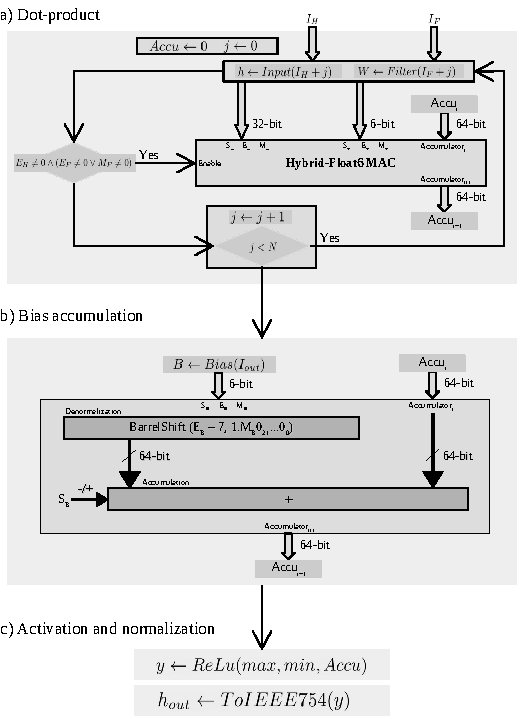
\includegraphics[width=0.5\columnwidth]{./chapters/cnn_accelerator/figures/dot_product_hybrid.pdf}
	\caption{(a) Dot-product hardware module with Hybrid-Float6 MAC, (b) bias accumulation, (c) activation and normalization.}
	\label{fig:dot_product_loop}
\end{figure*}

\subsubsection{Multiply-Accumulate}
The multiply-accumulate operation calculates the product of two numbers and adds the result to an accumulator. In FP arithmetics, the size of a hardware multiplier scales with the size of the mantissas. In the case of HF6, the 6-bit FP representation allows optimization in the mantissa multiplication. The 1-bit mantissa enables efficient MAC implementations by reducing the mantissa multiplication to a multiplexed addition, see \fig{fig:multiplier}. The denormalized results are accumulated in a fixed-point accumulator. This approach reduces latency, energy consumption, and resource utilization.

\begin{figure*}[b!]
	\centering
	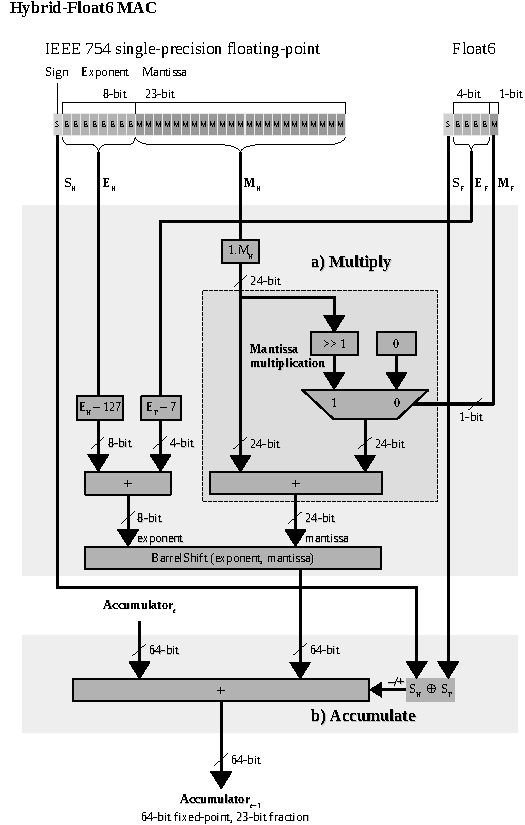
\includegraphics[width=0.5\columnwidth]{./chapters/cnn_accelerator/figures/multiplier.pdf}
	\caption{Hybrid-Float6 multiply-accumulate hardware design.}
	\label{fig:multiplier}
\end{figure*}

The Infinity and NaN special cases are not considered in this design since are not expected in ANN computation. For the subnormal case, the element-wise multiplication is disabled when having a zero entry and is approximated when having subnormal mantissa. The feature map values are considered zero when the exponent is zero ($E_H=0$). The filter values are considered zero when both exponent and mantissa are zero ($E_F=0\land M_F=0$). See \Fig{fig:dot_product_loop}(a). In the 6-bit FP, the 1-bit mantissa has one subnormal case, which is handled as a normalized case. This exploits the intrinsic error tolerance of ANN to reduce the hardware design.

The approximation error is defined by the difference between \Equ{eq:float} and \Equ{eq:float_subnorm} when $E=0$ and $M=2^{-1}$. The result defines the error as $e=2^{-B-1}$. Then, from \Equ{eq:float_bias} with $E_{size}=4$, we have $B=7$. Hence, $e=3.9\mathrm{e}{-3}$. This error is produced when having the subnormal case $E=0$ and $M=2^{-1}$, which corresponds to the value $\pm7.8\mathrm{e}{-3}$ deviated to $\pm1.17\mathrm{e}{-2}$. This approximation leverages the intrinsic error tolerance of ANN to reduce hardware resource utilization and energy consumption \cite{du2014leveraging}.


\subsubsection{On-Chip Memory Utilization}
\label{sec:memory_utilization}
The total on-chip memory utilization on the TP is defined by \Equ{eq:tp_memory}, where $TP_B$ and $V_{M}$ represent the tensor buffers and local variables (memory) required for the design, respectively. \Equ{eq:tp_memory_buffer} defines the tensor buffers, where $Input_{M}$ is the \emph{input buffer}, $Filter_{M}$ is the \emph{filter buffer}, $Bias_{M}$ is the \emph{bias buffer}. The on-chip memory buffers are defined in bits. \fig{fig:accelerator_buffers} illustrates the convolution operation utilizing the on-chip memory buffers.
\begin{figure*}[b!]
	\centering
	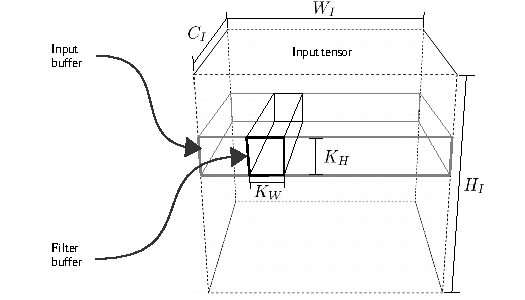
\includegraphics[width=0.5\columnwidth]{./chapters/cnn_accelerator/figures/accelerator_buffers.pdf}
	\caption{Design parameters for on-chip memory buffers on the TP.}
	\label{fig:accelerator_buffers}
\end{figure*}
\begin{eqnarray} \label{eq:tp_memory}
TP_{M}=TP_B+V_{M}
\end{eqnarray}
\begin{eqnarray} \label{eq:tp_memory_buffer}
TP_{B}=Input_{M}+Filter_{M}+Bias_{M}
\end{eqnarray}

The memory utilization of \emph{input buffer} is defined by \Equ{eq:input_memory}, where $K_{H}$ is the height of the convolution kernel, $W_{I}$ is the width of the input tensor, $C_{I}$ is the number of input channels, and $BitSize_{I}$ is the bit size of input tensor.
\begin{eqnarray} \label{eq:input_memory}
Input_{M}=K_{H}W_{I}C_{I}BitSize_{I}
\end{eqnarray}

The memory utilization of \emph{filter buffer} is defined by \Equ{eq:filter_memory}, where $K_{W}$ and $K_{H}$ are the width and height of the convolution kernel, respectively; $C_{I}$ and $C_{O}$ are the number of input and output channels, respectively; and $BitSize_{F}$ is the bit size of filter values.
\begin{eqnarray} \label{eq:filter_memory}
Filter_{M}=C_{I}K_{W}K_{H}C_{O}BitSize_{F}
\end{eqnarray}

The memory utilization of \emph{bias buffer} is defined by \Equ{eq:bias_memory}, where $C_{O}$ is the number of output channels, and $BitSize_{B}$ is the bit size of bias values.
\begin{eqnarray} \label{eq:bias_memory}
Bias_{M}=C_{O}BitSize_{B}
\end{eqnarray}

As a design trade-off, \Equ{eq:channel_in_memory} defines the capacity of output channels based on the given design parameters. The total on-chip memory $TP_{M}$ determines the TP capacity.
\begin{eqnarray} \label{eq:channel_in_memory}
C_{O}=\frac{TP_{M}-V_{M}-K_{H}W_{I}C_{I}BitSize_{I}}{C_{I}K_{W}K_{H}BitSize_{F}+BitSize_{B}}
\end{eqnarray}

The floating-point formats implemented in the TP are defined by $BitSize_F$, $BitSize_B$ and $BitSize_I$. The HF6 defines 6-bit for $BitSize_F$ and $BitSize_B$, and 32-bit for $BitSize_I$. These are design parameters defined before hardware synthesis. This allows fine control of BRAM utilization, which is suitable for resource-limited devices.

\subsection{Training Method}
The models are trained and quantized in separate stages.
\subsubsection{Training with Iterative Early Stop}
To achieve better performance on CNN-regression models, we implement a training procedure with iterative early stop cycle. This allows to reach better local minima. This is a four steps process:

\begin{enumerate}
	\item A model is obtained with an initial training with standard early stop monitoring.
	\item The model is iteratively re-trained with standard early stop to search for better local minima. In each early stop the Adam optimizer restarts the moving averages.
	\item In case of a better local minimum, the base model is updated/saved and used for subsequent re-training iterations, otherwise it is discarded.
	\item The cyclic process stops automatically with a given patience. This allows to set a maximum training iterations before the stop.
\end{enumerate}

This method is described in \Algo{alg:training}.

\subsubsection{Quantization Aware Training}
The quantization aware training (QAT) method is integrated into the training process, this operates after each mini-batch update. The quantization is applied on the trainable parameters of convolution layers. This method is implemented as a callback function in the TensorFlow/Keras framework, see \Algo{alg:quantization_integration}.

The quantization method uses rounding strategy to reduce the FP representation. This maps the full precision FP values to the closest representable 6-bit FP values, see \Algo{alg:quantize_training}. This method quantizes the filter and bias tensors of the convolution layers. We have observed that the exponent bit size plays a more predominant influence on the model accuracy than the mantissa bit size. In \cite{lai2017deep}, Lai et al. demonstrated that 4-bit exponent is adequate and consistent across different networks (SqueezeNet, AlexNet, GoogLeNet, VGG-16). In this work, we investigate 4-bit exponent and 1-bit mantissa.

\begin{algorithm}[h!]
	\caption{Training with iterative early stop cycle.}
	\label{alg:training}
	\begin{algorithmic}
		\SetAlgoLined
		\renewcommand{\algorithmicrequire}{\textbf{input:}}
		\renewcommand{\algorithmicensure}{\textbf{output:}}
		\REQUIRE $MODEL$ as the input model.
		\REQUIRE $D_{train}$ as the training data set.
		\REQUIRE $D_{val}$ as the validation data set.
		\REQUIRE $N_{I}$ as the stop patience for iterative training cycle.
		\REQUIRE $N_{E}$ as the early stop patience (epochs) for training.
		\REQUIRE $B_{size}$ as the mini-batch size.
		\ENSURE $MODEL$ as the full-precision output model.
		\STATE $Train(MODEL, D_{train}, D_{val}, N_{E}, B_{size})$
		\STATE $mse_i \gets Evaluate(MODEL, D_{val})$ // Benchmark
		\STATE $n_i \gets 0$
		\WHILE {$n_i<N_I$}
		\STATE // Iterative early stop cycle
		\STATE $Train(MODEL, D_{train}, D_{val}, N_{E}, B_{size})$
		\STATE $mse_v \gets Evaluate(MODEL, D_{val})$
		\IF{$mse_v < mse_i$}
		\STATE $Update(MODEL)$
		\STATE $mse_i \gets mse_v$
		\ELSE
		\STATE $MODEL  \gets LoadPreviousModel()$
		\STATE $n_I \gets n_I + 1$
		\ENDIF
		\ENDWHILE
	\end{algorithmic}
\end{algorithm}


\begin{algorithm}[h!]
	\caption{OnMiniBatchUpdate\_Callback.}
	\label{alg:quantization_integration}
	\begin{algorithmic}
		\SetAlgoLined
		\renewcommand{\algorithmicrequire}{\textbf{input:}}
		\renewcommand{\algorithmicensure}{\textbf{output:}}
		\REQUIRE $MODEL$ as the full-precision input model.
		\REQUIRE $E_{size}$ as the target exponent bits size.
		\REQUIRE $M_{size}$ as the target mantissa bits size.
		\REQUIRE $D_{train}$ as the training data set.
		\REQUIRE $D_{val}$ as the validation data set.
		\REQUIRE $N_{ep}$ as the number of epochs.
		\REQUIRE $B_{size}$ as the mini-batch size.
		\ENSURE $MODEL$ as the quantized output model.
		\STATE //Quantize
		\STATE $MODEL \gets \Algo{alg:quantize_training}(MODEL,E_{size}, M_{size})$ 
		\IF {$1<epoch$}
		\STATE // Update model after first epoch
		\STATE $mse_v \gets Evaluate(MODEL, D_{val})$
		\IF{$mse_v < mse_i$}
		\STATE $Update(MODEL)$
		\STATE $mse_i \gets mse_v$
		\ENDIF
		\ENDIF
	\end{algorithmic}
\end{algorithm}

\begin{algorithm}[h!]
	\caption{Custom floating-point quantization.}
	\label{alg:quantize_training}
	\begin{algorithmic}
		\SetAlgoLined
		\renewcommand{\algorithmicrequire}{\textbf{input:}}
		\renewcommand{\algorithmicensure}{\textbf{output:}}
		\REQUIRE $MODEL$ as the CNN.
		\REQUIRE $E_{size}$ as the target exponent bit size.
		\REQUIRE $M_{size}$ as the target mantissa bits size.
		\REQUIRE $STDM_{size}$ as the IEEE 754 mantissa bit size.
		\ENSURE $MODEL$ as the quantized CNN.
		\FOR {$layer$ in $MODEL$}
		\IF {$layer$ is $Conv2D$ or $SeparableConv2D$}
		\STATE $filter, bias \gets GetWeights(layer)$
		\FOR {$x$ in $filter$ and $bias$}
			\STATE $sign \gets GetSign(x)$
			\STATE $exp \gets GetExponent(x)$
			\STATE $fullexp \gets 2^{E_{size}-1}-1$ // Get full range value
			\STATE $cman \gets GetCustomMantissa(x, M_{size})$
			\STATE $leftman \gets GetLeftoverMantissa(x, M_{size})$
			\IF {$exp <-fullexp$}
				\STATE$x\gets0$
			\ELSIF{$exp > fullexp$}
				\STATE$x\gets (-1)^{sign}\cdot2^{fullexp}\cdot(1+(1-2^{-M{size}}))$
			\ELSE
				\IF {$2^{STDM_{size}-M_{size}-1}-1<leftman$}
					\STATE $cman \gets cman+1$ // Above halfway
					\IF{$2^{M_{size}}-1<cman$}
					\STATE $cman \gets 0$ // Correct mantissa overflow
					\STATE $exp \gets exp + 1$
					\ENDIF
				\ENDIF
				\STATE // Build custom quantized floating-point value
				\STATE$x\gets (-1)^{sign}\cdot2^{exp}\cdot(1+cman\cdot2^{-M_{size}})$
			\ENDIF
		\ENDFOR
		\STATE $SetWeights(layer, filter, bias)$
		\ENDIF
		\ENDFOR
	\end{algorithmic}
\end{algorithm}
\begin{figure*}[b!]
	\centering
	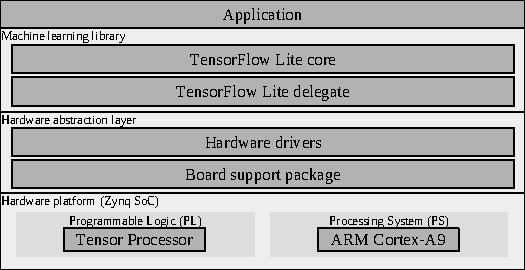
\includegraphics[width=0.5\columnwidth]{./chapters/cnn_accelerator/figures/sw_stack.pdf}
	\caption{Base embedded software architecture.}
	\label{fig:sw_stack}
\end{figure*}
\subsection{Embedded software architecture}
The software architecture is a layered object-oriented application framework written in C++, see \fig{fig:sw_stack}. A description of the software layers is as follows:
\begin{itemize}
	\item \emph{Application}: As the highest level of abstraction, this software layer implements the application invoking the ML library.
	\item \emph{Machine learning library}: This layer consist of TensorFlow Lite for micro controllers. This offers a comprehensive high level API that allows ML inference. This provides delegate software interfaces for custom hardware accelerators.
	\item \emph{Hardware abstraction layer}: This layer consist of the hardware drivers to handle initialization and runtime operation of the TP and DMA.
\end{itemize}
\section{Experimental Results}
\label{sec:experimental_results}
This section presents experimental results using a low-power/low-cost sensor analytics application. A \gls{cnn}-regression model is proposed to predict x- y- coordinates of acoustic emissions based on piezoelectric vibrations. Quantitative and qualitative aspects of the analytics are compared using floating-point 32-bit, fixed-point 8-bit, Hybrid-Logarithmic 6-bit, and Hybrid-Float6.

To demonstrate the proposed concept, the \gls{cnn} model is deployed in the smallest Zynq \gls{soc} \gls{fpga} device for low-power inference. The performance of the \gls{tp} synthesized with standard \gls{fp} (using Xilinx LogiCORE IPs) and Hybrid-Float6 design.

\subsection{Sensor Analytics Application}
The analytics model is designed to predict x- y- coordinates of acoustic emissions on a metal plate. The metal plate is in the presence of noise disturbance to simulate realistic conditions. This subsection presents the structure for experimental setup, data sets, and the \gls{cnn}-regression model.

\subsubsection{Experimental Setup}
The experiment uses eight piezoelectric sensors (Vallen Systeme VS900) attached with magnetic holders on a metal plate ($\unit[90]{cm}\times\unit[86.6]{cm}\times\unit[0.3]{cm}$). The VS900 devices can operate either in active or passive mode. Six VS900 are used in passive mode as acoustic sensors and two in active mode to produce acoustic emissions. These acoustic emissions simulate anomalies on x- y- coordinates as well as the noise disturbance on the system. See \fig{fig:data_set}(a). To create data sets, the samples of acoustic emissions are labeled with their coordinates.

\subsubsection{Data Sets}
The data sets are recorded applying pulses on the metal plate, the x- y- coordinates of these pulses are used as labels. The pulses for training and validation data sets are shown in \fig{fig:data_set}(b) and \fig{fig:data_set}(c), respectively. The pulses for training and validation data sets are mutually exclusive, this exclusion is represented by the cross symbols in \fig{fig:data_set}(c). This creates a grid layout used to collect samples for the data sets. This grid is $10\times10$ divisions, these are on the metal plate area ($\unit[90]{cm}\times\unit[86.6]{cm}$). This grid does not consider the four corners as they are used for magnetic holders.

\begin{figure}[t!]
	\centering
	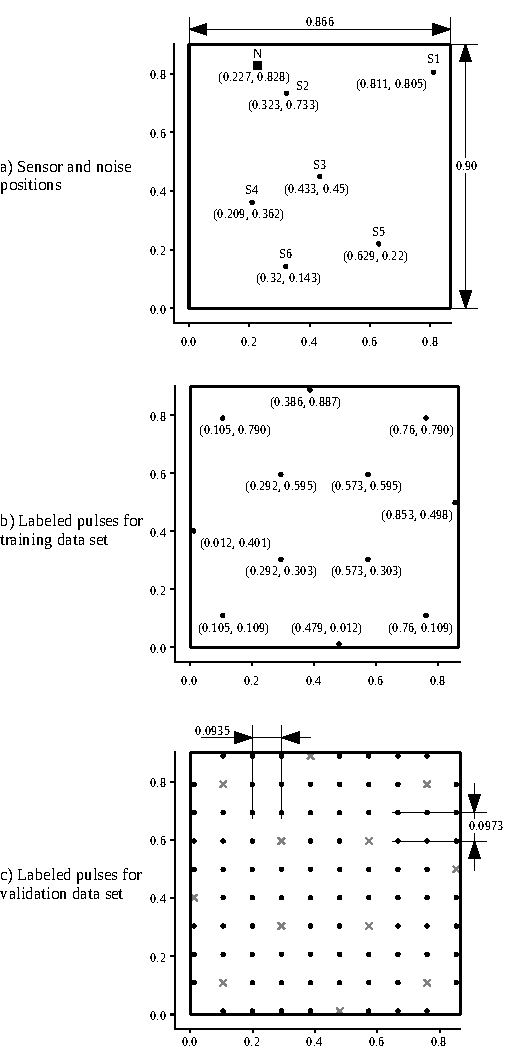
\includegraphics[width=0.5\textwidth]{./chapters/cnn_accelerator/figures/histograms/data_set.pdf}
	\caption{Experimental setup for sensor analytics on structural health monitoring, all lengths are in meters (m).}
	\label{fig:data_set}
\end{figure}

In order to create reproducible acoustic emissions, this demonstration uses 9-cycle sine pulse in a Hanning window with central frequency $f_\mathrm{c}$ (narrow-banded in the frequency domain). This experiment assumes guided Lamb waves based on the plate structure. The narrow-band behavior also reduces the dispersion of the acoustic emission waves~\cite{hannwindowsine}. The waveform can be expressed as a function of time $t$ as follows:

\begin{equation}
x_\mathrm{pulse}(t) = \frac{1}{2} \Big(1-\cos{\frac{f_\mathrm{c} t}{5}} \Big) A_0 \sin{f_\mathrm{c} t}.
\end{equation}

To generate the data sets, slightly different pulse amplitudes and frequencies for excitation are used. The pulse frequency $f_c$ is varied in $\unit[1]{kHz}$ steps between $\unit[300]{kHz}$ and $\unit[349]{kHz}$ and the amplitude $A_0$ is varied in $\unit[0.1]{V}$ steps between $\unit[2.6]{V}$ and $\unit[3.5]{V}$. This produces 500 different pulses for each of the excitation points.

The signals for labeled pulses and noise disturbance are generated by \glspl{awg}. The sensor signals are recorded via a Vallen AMSY-6 measurement system with a resolution of 18 bits and a sampling rate of $f_\mathrm{S} =\unit[10]{MHz}$. The disturbance signal is gaussian noise with amplitudes between 0-3 V. This noise is applied via the piezoelectric device $N$ at $x=\unit[0.227]{m}$ and $y=\unit[0.828]{m}$, see \fig{fig:data_set}(a).

To obtain frequency components, the sampled pulses are converted into the frequency-time domain using the \gls{stft}. This is calculated as follows~\cite{stft_lit}:

\begin{flalign}
\label{stft_eq2}
\mathcal{F}_{m,k}^\gamma= \sum_{n=0}^{N-1} x[n] \cdot \gamma^*[n-m\Delta M]\cdot \mathrm{e}^{\frac{-j 2 \pi k n }{N}}
\end{flalign}

Here $x[n]$ describes a discrete-time signal and $\gamma^*[n-m\Delta M]\cdot \mathrm{e}^{\frac{-j 2 \pi k n }{N}}$ the time- and frequency-shifted window function inside the considered interval $[0 , N-1]$. $\Delta M$ describes the time shift and $N$ the transformation window. Since only discrete frequencies and time points are considered, $m = 0,1,...,M-1$ is valid. For pictorial representation, the magnitude of the complex-valued \gls{stft} is employed in a spectrogram $\mathcal{S}_{m,k}$:

\begin{flalign}
\label{stft_eq3}
\mathcal{S}_{m,k}= \left|\mathcal{F}_{m,k}^\gamma\right|^2 = \left|\sum_{n=0}^{N-1} x[n] \cdot \gamma^*[n-m\Delta M]\cdot \mathrm{e}^{\frac{-j 2 \pi k n }{N}} \right|^2
\end{flalign}

In addition, these spectrograms are scaled in decibels. The spectrogram in decibels $\mathcal{S}_{m,k,\mathrm{dB}}$ produces $\mathcal{S}_{m,k,\mathrm{dB}}= 20 \cdot \mathrm{log}_{10}(\mathcal{S}_{m,k})$. For conversion of data, the experiment uses a signal length of 400 \textmu s (75 \textmu s pretrigger and 325 \textmu s post trigger). Thus, the arrival times of the pulses are included in the spectrogram for all channels and labeled positions. This uses Blackman window function~\cite{blackman_window}, \gls{fft} length of 32 samples, and overlap of 8 samples. The spectrograms are calculated for frequencies in the range of \unit[100]{kHz} to \unit[500]{kHz}. This produces a spectrogram size of 8x16 (8 frequency bins, 16 time values).

In order to generate larger data sets, four further variants are created with time shifts of 15 \textmu s/ 30 \textmu s/ 45 \textmu s/ 60 \textmu s. Subsequently, all spectrograms are converted to grayscale with scaling between \unit[-100]{dB} and \unit[-40]{dB}, see \fig{fig:spectrograms}.

In overall, the data set has a size of 1,440,000 images. This is the result of 500 (pulses) $\cdot$ 5 (spectrograms) $\cdot$ 6 (listening sensors) $\cdot$ 96 (excitation points).

\begin{figure}[t!]
	\centering
	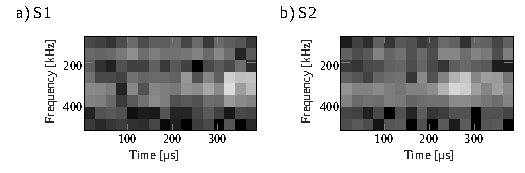
\includegraphics[width=0.5\textwidth]{./chapters/cnn_accelerator/figures/histograms/spectrograms.pdf}
	\caption{Spectrograms of sensors $S_1, S_2$ converted to grayscale for pulses at $x =0.105$ m, $y = 0.109$ m with noise disturbance.}
	\label{fig:spectrograms}
\end{figure}

\subsubsection{CNN-Regression Model}
The data analytics is implemented with a \gls{cnn}-regression model, see \fig{fig:model}. The structure of the model is described below:

\begin{enumerate}[label=\alph*)]
\item Input tensor. This is composed of spectrograms from the sensor signals. The tensor shape is defined by $S \times T \times F$, where $S$ is the number of sensors, and $T \times F$ is the time-frequency resolution of the spectrograms, see \fig{fig:model}(a).

\item Feature extraction. This is composed of three blocks of convolution, batch normalization, and max-pooling layers, see \fig{fig:model}(b). The number of channels in the convolution layers are defined by the hyper-parameters $A$, $B$, and $C$.

\item Regression function. This is an arbitrary function implemented with two fully connected layers and an output layer with linear activation, see \fig{fig:model}(c).
\end{enumerate}


\begin{figure}[t!]
	\centering
	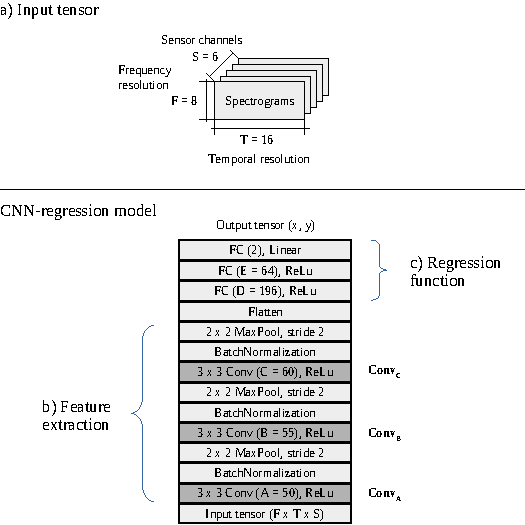
\includegraphics[width=0.5\textwidth]{./chapters/cnn_accelerator/figures/models.pdf}
	\caption{CNN-regression model for sensor analytics.}
	\label{fig:model}
\end{figure}


\subsection{Training}
\subsubsection{Base Model}
The model in \fig{fig:model} is trained using Adam algorithm with iterative search. The Adam optimizer is configured with the default settings presented in \cite{kingma2014adam}: $\alpha = 0.001$, $\beta_1 = 0.9$, $\beta_2 = 0.999$, and $\epsilon = 1\mathrm{e}{-8}$. The training-cycle has a patience of 10 iterations before stop, the optimizer is executed with early stop patience of 10 epochs, and mini-batch size of 512 samples. This is applied using the method described in \Algo{alg:training} with $N_I = 10$, $N_E=10$, $B_{size}=512$.

The training results are illustrated in \fig{fig:optimization}(a). In this optimization, the initial and the final models achieve $MSE=\unit[0.0135]{m^2}$ and $MSE=\unit[0.0122]{m^2}$, respectively. The $MSE$ is calculated with the Euclidean distance (loss) between the real/expected and the predicted/inferred coordinates. The initial model is obtained at the first early stop (after 10 epochs). In each stop, the moving averages of the Adam optimizer get re-initialized. This facilitates searching for better local minima. The model gets saved/updated when finding a better minimum.

\begin{figure}[h!]
	\centering
	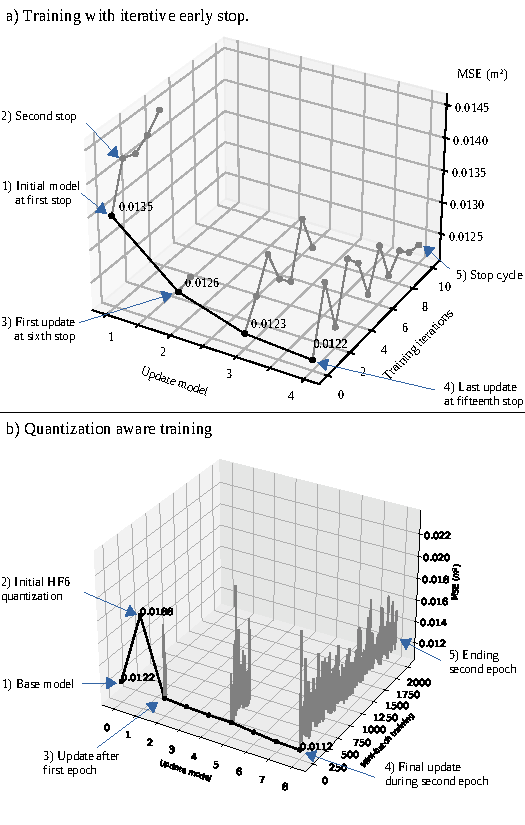
\includegraphics[width=0.5\textwidth]{./chapters/cnn_accelerator/figures/histograms/training_and_quantization.pdf}
	\caption{Training results.}
	\label{fig:optimization}
\end{figure}

The final model achieves $MSE=\unit[0.0122]{m^2}$, which corresponds to $MAE=\unit[0.0955]{m}$. See \fig{fig:model_evaluation}(a). In total, the training takes 379 epochs in 25 cycle-search iterations. The first search takes 43 epochs for the initial model and subsequent search iterations take an average of 14 epochs. The total time is 53 minutes using a \gls{pc} with AMD Ryzen 5 5600H and NVIDIA GeForce RTX 3050 \gls{gpu}.

\begin{figure}[h!]
	\centering
	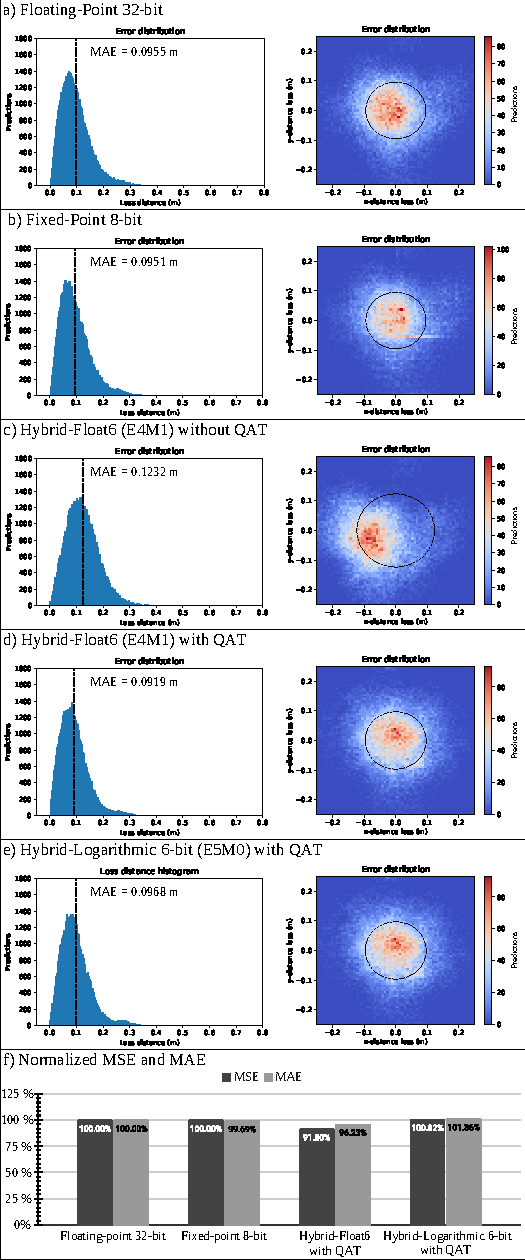
\includegraphics[width=0.5\textwidth]{./chapters/cnn_accelerator/figures/histograms/model_evaluation.pdf}
	\caption{Performance of the model with different data representations.}
	\label{fig:model_evaluation}
\end{figure}

\subsubsection{TensorFlow Lite 8-bit Quantization}
This optimization method converts filter and bias tensors as well as activation maps to 8-bit integer representation, this allows inference using integer-only arithmetic~\cite{hannwindowsine}. In this research, this quantization is applied only to the convolution layers as they are the compute bound operations. Other layers employ 32-bit \gls{fp} representation.

In the compute graph, the input and output feature maps are glued with linear quantization at the input and output of the \emph{Conv2D} operations.

The base model is quantized using the TensorFlow Lite library with integer-only quantization on the \emph{Conv2D} tensor operations. The filter and bias tensors are represented by 8-bit and 32-bit signed integers, respectively. The input and output activation maps are represented by 8-bit signed integer. The TensorFlow quantization includes two additional vectors (output-multiplier and output-shift coefficients), these two vectors are the same shape as the bias vector with 32-bit integer representation.

This model achieves $MSE=\unit[0.0126]{m^2}$ and $MAE=\unit[0.0992]{m}$. See \fig{fig:model_evaluation}(b). The MAE increases 5.1\% of the base model. We attribute this degradation to the 8-bit quantization on the \emph{Conv2D} layers.

\subsubsection{Inference of non-quantized models on HF6 hardware}
To demonstrate backward compatibility, the inference quality of the base model is measured without quantization on the \gls{hf6} hardware. See \fig{fig:model_evaluation}(c). This obtains $MSE=\unit[0.0188]{m^2}$ and $MAE=\unit[0.1232]{m}$. The MAE increases 29.5\% of the base model. We attribute this degradation to the rounding errors of non-quantized filters and bias in \emph{Conv2D} layers.

\subsubsection{Quantization-Aware Training for HF6 hardware}
The \gls{qat} is a post-training optimization. This has been run during two epochs with mini-batch size of 10 samples. This quantization is executed targeting the HF6 format: 4-bit exponent and 1-bit mantissa. This is applied to filter and bias tensors of \emph{Conv2D} layers. This method is described in \Algo{alg:quantization_integration} with $N_{ep}=2$, $B_{size}=10$, $E_{size}=4$, $M_{size}=1$. The optimization results are illustrated in \fig{fig:optimization}(b).

The resulting model achieves $MSE=\unit[0.0112]{m^2}$ and $MAE=\unit[0.0919]{m}$. This corresponds to an error reduction of 8.2\% and 3.77\%, respectively. We attribute this improvement to the regularization effect. See \fig{fig:model_evaluation}(d). The \gls{qat} time is 185 minutes.


\subsubsection{Quantization-Aware Training for Hybrid-Logarithmic 6-bit}
For the sake of quality comparison with logarithmic quantization, the model with 6-bit logarithmic representation is generated. See \fig{fig:floating}(e). This quantization matches the bit size of \gls{hf6}. The filter and bias tensors of \emph{Conv2D} layers are quantized with the 6-bit logarithmic format: 1-bit sign, 5-bit signed exponent, and 0-bit mantissa. This is applied using the method described in \Algo{alg:quantization_integration} with $N_{ep}=2$, $B_{size}=10$, $E_{size}=5$, $M_{size}=0$.

The model achieves $MSE=\unit[0.0123]{m^2}$ and $MAE=\unit[0.0968]{m}$, which correspond to an error increase of 0.82\% and 1.36\%, respectively. We attribute this degradation to the 6-bit logarithmic quantization lacking fractional bits. See \fig{fig:model_evaluation}(e).

A summary of improvement-degradation of MSE and MAE with different data representations is presented in \fig{fig:model_evaluation}(f).

\subsection{Hardware Design Exploration}
The proposed hardware/software co-design is demonstrated on the Zynq-7007S \gls{soc} on the MiniZed development board. This \gls{soc} integrates a single ARM Cortex-A9 \gls{ps} and a \gls{pl} equivalent to Xilinx Artix-7 \gls{fpga} in a single chip~\cite{xilinx2015zynq}. The Zynq-7007S \gls{soc} architecture maps the custom logic and software in the \gls{pl} and \gls{ps}, respectively.

In this platform, the proposed hardware/software architecture is implemented to deploy the sensor analytics application. The desired model is converted to TensorFlow Lite (floating-point) and deployed on the embedded software as a hex dump as a C array. The Zynq-7007S \gls{soc} executes inference with TensorFlow Lite on the \gls{ps}. The computational workload of convolution layers is delegated to the dedicated hardware.

\subsubsection{Benchmark on Embedded CPU}
First, the performance of the embedded \gls{cpu} is explored for inference without hardware acceleration. In this case, TensorFlow Lite creates the \gls{cnn} model as a sequential compute graph executing all computation on the \gls{cpu} (ARM Cortex-A9) at $\unit[666]{MHz}$ with power dissipation of $\unit[1,187]{W}$.

The compute performance and run-time inference of the \gls{cpu} are shown in \Tab{tab:performance}(a) and \fig{fig:runtime}(a), respectively.

\subsubsection{Benchmark on Tensor Processor Synthesized with Xilinx LogiCORE IP for Floating-Point Computation}
For this design, the TP is implemented with standard Xilinx \gls{fp} hardware prior synthesis. The design parameters for the maximum required accelerator on-chip size are:
\begin{itemize}
	\item Max convolution kernel size: $K_W = K_H = 3$.
	\item Max input tensor width: $W_I = 16$.
	\item Max input and output channels: $C_I = 55$, $C_O = 60$.
	\item Filter and bias bit size: $BitSize_F=BitSize_B=32$.
	\item Input tensor bit size: $BitSize_I=32$.
\end{itemize}

Using equations from Section \ref{sec:memory_utilization}, the on-chip memory utilization are $Input_M=84,480$b, $Filter_M=950,400$b, and $Bias_M=1,920$b. Hence, the required on-chip memory buffer size is $TP_B=1,036,800$b.

The post-implementation resource utilization and power dissipation are presented in \Tab{tab:resource_utilization}(a). The complete hardware platform utilizes 83\% of BRAM, this includes the on-chip memory requirements of the \gls{tp}, \gls{dma}, and AXI interconnects. The total available on-chip memory (BRAM) on the Zynq-7007S \gls{soc} is $\unit[1.8]{Mb}$. After hardware syntheses, the estimated power dissipation of the \gls{tp} is $\unit[85]{mW}$ at $\unit[200]{MHz}$ (this estimation is provided by Xilinx Vivado).

\begin{table}[!h]\centering
	\caption{Resource utilization and power dissipation on the Zynq-7007S SoC.}\label{tab:resource_utilization}
	\scriptsize
	\begin{tabular}{lrrrrrr}\toprule
		\multirow{2}{*}{\textbf{TP engine}} &\multicolumn{4}{c}{\textbf{Post-implementation resource utilization}} &\multirow{2}{*}{\textbf{Power (W)}} \\\cmidrule{2-5}
		&\textbf{LUT} &\textbf{FF} &\textbf{DSP} &\textbf{BRAM 36Kb} & \\\midrule
		\multirow{2}{*}{(a) Floating-Point} &5,578 &8,942 &23 &41.5 &\multirow{2}{*}{1.429} \\
		&39\% &31\% &35\% &\textbf{83\%} & \\
		\multirow{2}{*}{(b) Hybrid-Float6} &7,313 &10,330 &20 &15 &\multirow{2}{*}{1.424} \\
		&51\% &36\% &30\% &\textbf{30\%} & \\
		\bottomrule
	\end{tabular}
\end{table}

The compute performance and inference schedule of the model on this hardware implementation are shown in \Tab{tab:performance}(b) and \fig{fig:runtime}(b), respectively. During run-time, the software (TensorFlow Lite) delegates computation to the \gls{tp} as dedicated hardware for \emph{Conv2D} tensor operations.

The implementation of the dot-product with standard \gls{fp} engine (IEEE 754 arithmetic) utilizes proprietary multiplier and adder floating-point operator cores. Vivado \gls{hls} implements \gls{fp} arithmetic operations by mapping them onto Xilinx LogiCORE IP cores, these \gls{fp} operator cores are instantiated in the resultant \gls{rtl}~\cite{hrica2012floating}. In this case, the implementation of the dot-product with the standard \gls{fp} computation reuses the multiplier and adder cores in different compute sections of the \gls{tp}. The post-implementation resource utilization and power dissipation of the individual floating-point operator cores are shown in \Tab{tab:LogiCORE}.

\begin{table}[!t]\centering
	\caption{Compute performance of the CPU and TP on each Conv2D tensor operation. This table presents: tensor operation, computational cost in mega floating-point operations (MFLOP), latency, throughput, power efficiency, and estimated energy consumption as the energy delay product (EDP).}\label{tab:performance}
	\scriptsize
	\begin{tabular}{lrrrrrr}\toprule
		\textbf{Operation} &\textbf{MFLOP} &\textbf{t (ms)} &\textbf{MFLOP/s} &\textbf{MFLOP/s/W} &\textbf{EDP (mJ)} \\\midrule
		& &\multicolumn{4}{l}{\textbf{a) CPU (ARM Cortex-A9) @666MHz, 1.187 W}} \\
		Conv\textsubscript{A} &0.691 &112.24 &6.16 &5.19 &133.23 \\
		Conv\textsubscript{B} &1.584 &213.13 &7.43 &6.26 &252.99 \\
		Conv\textsubscript{C} &0.475 &46.59 &10.20 &8.59 &55.31 \\
		& &\multicolumn{4}{l}{\textbf{b) TP (Floating-Point engine) @200MHz, 85 mW}} \\
		Conv\textsubscript{A} &0.691 &12.49 &55.34 &651.11 &1.06 \\
		Conv\textsubscript{B} &1.584 &16.39 &96.66 &1,137.20 &1.39 \\
		Conv\textsubscript{C} &0.475 &3.59 &132.44 &1,558.13 &0.30 \\
		& &\multicolumn{4}{l}{\textbf{c) TP (Hybrid-Float6 engine) @200MHz, 84 mW}} \\
		Conv\textsubscript{A} &0.691 &6.92 &99.81 &1,188.24 &0.58 \\
		Conv\textsubscript{B} &1.584 &4.41 &358.94 &4,273.09 &0.37 \\
		Conv\textsubscript{C} &0.475 &0.99 &482.44 &5,743.29 &0.08 \\
		\bottomrule
	\end{tabular}
\end{table}

\begin{figure}[t!]
	\centering
	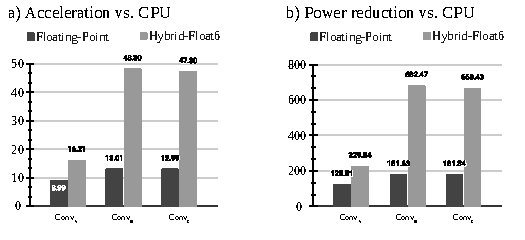
\includegraphics[width=0.5\textwidth]{./chapters/cnn_accelerator/figures/power_breakdown/acceleration_power_reduction.pdf}
	\caption{Inference acceleration and power reduction on the TP with floating-point and HF6 vs. CPU on the Zynq-7007S SoC.}
	\label{fig:acceleration}
\end{figure}


\begin{table}[!h]\centering
	\caption{Resource utilization and power dissipation of individual multiplier and adder floating-point (IEEE 754) operator cores (Xilinx LogiCORE IP).}\label{tab:LogiCORE}
	\scriptsize
	\begin{tabular}{lrrrrrr}\toprule
		\textbf{Core operation} &\textbf{DSP} &\textbf{FF} &\textbf{LUT} &\textbf{Latency (clk)} &\textbf{Power (mW)} \\\midrule
		Multiplier &3 &151 &325 &4 &7 \\
		Adder &2 &324 &424 &8 &6 \\
		\bottomrule
	\end{tabular}
\end{table}



\subsubsection{Tensor Processor Synthesized with Hybrid-Float6 Hardware Architecture}
To demonstrate the proposed design, the \gls{tp} with \gls{hf6} hardware reuses the standard \gls{fp} design parameters with the following variation for the 6-bit representation in filter and bias: $BitSize_F=BitSize_B=6$.

Using equations from Section \ref{sec:memory_utilization}, the on-chip memory requirements for the hardware accelerator are $Input_M=\unit[84,480]{b}$, $Filter_M=\unit[178,200]{b}$, $Bias_M=\unit[360]{b}$. Hence, the required on-chip memory buffer size is $TP_B=\unit[263,040]{b}$.

The post-implementation resource utilization and power dissipation are presented in \Tab{tab:resource_utilization}(b). The complete hardware platform utilizes 30\% of BRAM, this includes the on-chip memory requirements of the \gls{tp}, \gls{dma}, and AXI interconnects. The estimated power dissipation of the \gls{tp} is $\unit[84]{mW}$ at $\unit[200]{MHz}$ (this estimation is provided by Xilinx Vivado).

The compute performance and inference schedule of the model on this hardware implementation are shown in \Tab{tab:performance}(c) and \fig{fig:runtime}(c), respectively. \Fig{fig:acceleration} presents a comparison of the acceleration and the reduction of power dissipation between standard \gls{fp} and \gls{hf6} hardware implementations.

This deployment does not require model treatment for hardware compatibility. For backward compatibility, the 6-bit \gls{fp} representation is wrapped into the standard \gls{fp}. The dedicated hardware design extracts the 6-bit format automatically to perform computation.

\begin{figure}[t!]
	\centering
	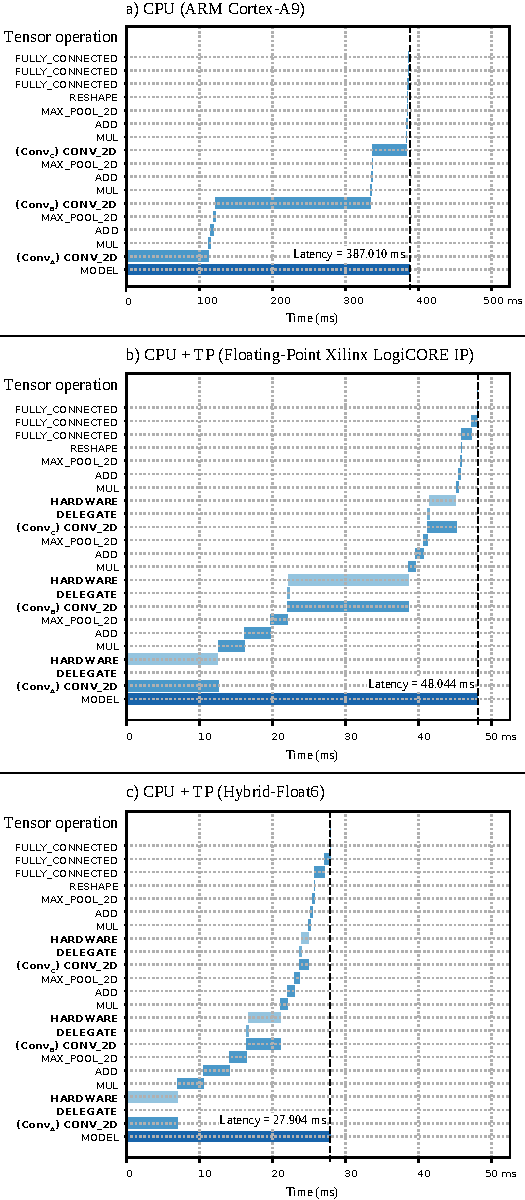
\includegraphics[width=0.5\textwidth]{./chapters/cnn_accelerator/figures/runtime/runtime.pdf}
	\caption{Run-time inference of TensorFlow Lite on the Zynq-7007S SoC. (a) CPU ARM Cortex-A9 at $\unit[666]{MHz}$, (b) cooperative CPU + TP with floating-point Xilinx LogiCORE IP at $\unit[200]{MHz}$, and (c) cooperative CPU + TP with Hybrid-Float6 at $\unit[200]{MHz}$.}
	\label{fig:runtime}
\end{figure}

\subsection{Discussion}
\subsubsection{Training and Quantization}
The training with iterative early stop obtains a model with enhanced accuracy than standard early stop. This method iteratively resets the moving averages of Adam's optimizer, which helps to iteratively search for better local minima. This iterative search is suitable for models with low computational cost.

The TensorFlow Lite 8-bit quantization preserves the overall model accuracy. In some cases, the associated regularization effect can improve the accuracy. However, the error distribution in \gls{cnn} linear regressions gets slightly degraded. In particular, 8-bit quantized output layers incur in discrete-degradation patterns, \fig{fig:2d_error_distribtion}(b) shows this effect on three different models. Vertical and horizontal patterns appear in the error distribution of 8-bit fixed-point quantization. We attribute this effect to the 8-bit resolution in the activation maps. In the case of \gls{hf6} quantization, the activation maps are represented by floating-point preventing this degradation.

The proposed 6-bit \gls{fp} representation (E4M1) improves latency, hardware area, and power dissipation, while preserving model accuracy. For comparison, in our application, this number format produces better results than the 6-bit logarithmic representation (E5M0). This is demonstrated in \Fig{fig:model_evaluation}(d) and \Fig{fig:model_evaluation}(e).

In \cite{lai2017deep}, Lai et al. demonstrated that 4-bit exponent and X-bit mantissa preserves accuracy on SqueezeNet, AlexNet, GoogLeNet, and VGG-16. To contribute on this, I investigated 4-bit exponent and 1-bit mantissa to ALL-CNN-C~\cite{springenberg2014striving}, this produces an accuracy degradation of 1.39\% and 0.11\% with \gls{qat}. While applying 6-bit logarithmic produces a degradation of 11.18\% and 7.22\% with \gls{qat}.

\begin{figure}[t!]
	\centering
	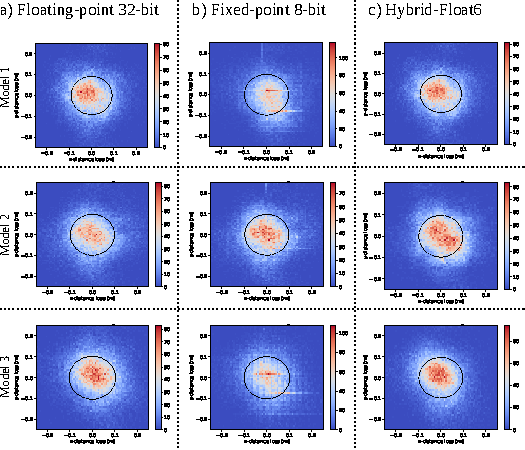
\includegraphics[width=0.5\textwidth]{./chapters/cnn_accelerator/figures/histograms/2D_error_distribtion.pdf}
	\caption{2D error distribution of three CNN-regression models.}
	\label{fig:2d_error_distribtion}
\end{figure}

\subsubsection{Implementation and Performance}
The proposed \gls{hf6} implementation reduces on-chip memory and \gls{dsp} utilization while slightly increasing \glspl{ff} and \glspl{lut} compared to the standard \gls{fp} implementation. See \Tab{tab:resource_utilization} and \Fig{fig:resource_utilization}. This is attributed to the \gls{hf6} logic implementation using \gls{ff} and \gls{lut}, while the \gls{fp} logic implementation uses Xilinx LogiCORE IPs mainly with \glspl{dsp}.

The compute performance of the \gls{cpu} and \gls{tp} on each convolution layer is presented in \Tab{tab:performance} and \fig{fig:acceleration}. 
The peak acceleration and power efficiency of the \gls{tp} with standard \gls{fp} (Xilinx LogiCORE IP) is $13\times$ and \unit[1,558.13]{MFLOPS/s/W}, respectively. While the peak acceleration and power efficiency of the \gls{tp} with \gls{hf6} is $48.3\times$ and \unit[5,743.29]{MFLOPS/s/W}, respectively. The \gls{hf6} hardware demonstrates an improvement of $3.7\times$ in acceleration and power efficiency with respect to the standard \gls{fp} hardware. See \Fig{fig:acceleration}.

The estimated power dissipation on the \gls{soc} is presented in \fig{fig:power}. This shows a very similar breakdown of power dissipation in both implementations. However, the energy efficiency is increased due to the reduced latency in \gls{hf6} hardware. A comparison of related work is presented in \Tab{tab:comparison}.

\begin{figure}[h!]
	\centering
	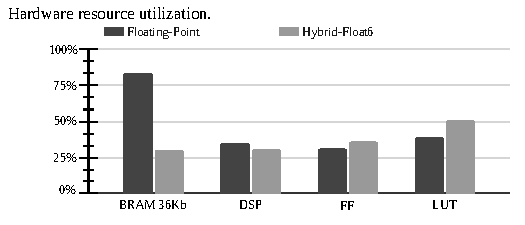
\includegraphics[width=0.5\textwidth]{./chapters/cnn_accelerator/figures/power_breakdown/resource_utilization.pdf}
	\caption{Hardware resource utilization on the Zynq-7007S SoC.}
	\label{fig:resource_utilization}
\end{figure}

\begin{figure}[h!]
	\centering
	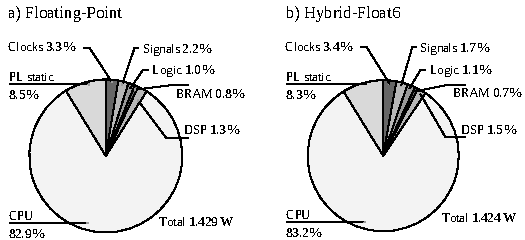
\includegraphics[width=0.5\textwidth]{./chapters/cnn_accelerator/figures/power_breakdown/power_breakdown.pdf}
	\caption{Estimated power dissipation on the Zynq-7007S SoC with PS at $\unit[666]{MHz}$ and PL at $\unit[200]{MHz}$.}
	\label{fig:power}
\end{figure}

The run-time inference of TensorFlow Lite on the \gls{soc} is illustrated in \Fig{fig:runtime}. This shows the convolution layers as the compute-bound operations. The proposed embedded platform is a cooperative system where the convolution operations are delegated to the dedicated hardware accelerator. The ARM \gls{cpu} obtains a latency of $\unit[387]{ms}$ ($\unit[2.58]{FPS}$). The platform with standard \gls{fp} hardware obtains a latency of $\unit[48]{ms}$ ($\unit[20.8]{FPS}$), while the implementation with \gls{hf6} obtains a latency of $\unit[27.9]{ms}$ ($\unit[35.84]{FPS}$). These represent an overall acceleration of $8\times$ and $13.87\times$ over the \gls{cpu}, respectively.

This design facilitates \gls{ml} compatibility/portability as the 6-bit \gls{fp} is wrapped in the standard \gls{fp} representation. The dedicated hardware design extracts the 6-bit format automatically and performs computation.

\subsubsection{SoC Design and Compatibility}
The proposed design is an alternative for high accuracy and low-power floating-point inference. The system runs as a cooperative hardware/software mechanism. This architecture delegates compute-bound tensor operations to a hardware accelerator.

The hybrid 32-bit \gls{fp} and 6-bit \gls{fp} quantization enables high quality of results and backward \gls{ml} compatibility. Backwards \gls{ml} compatibility gives portability from training to inference. This enables to run inference of \gls{hf6} quantized models on standard \gls{fp} hardware and vise versa. The proposed \gls{hf6} architecture allows to compute inference of non-quantized floating-point \gls{ml} models for rapid deployment; however, this will incur in accuracy degradation depending on the resilience of the model, see \Fig{fig:model_evaluation}(c).

\subsubsection{Limitations and Directions for Future Work}
In this research, we foresee three lines of future work:
\begin{itemize}
\item \textbf{To reduce energy consumption.} The proposed architecture consists of a hybrid floating-point quantization using 32-bit activation maps. These can be represented using lower-bit formats; for example, Bfloat16 and 8-bit or lower custom floating-point. This would reduce hardware resource utilization, memory footprint and data transfer, while preserving backward compatibility and accuracy. (Floating-point formats present better \gls{qor} than fixed-pint representations based on the dynamic value range.)

\item \textbf{To increase performance.} This implementation requires matching higher computational throughput with memory bandwidth. This would replace the light-weight pipeline hardware design with a parallelized structure. This will increase hardware area and energy consumption. This can be achieved by using wider memory channels and systolic arrays to increase throughput.

\item \textbf{To use in computer vision applications.} This implementation is designed for sensor analytics workloads. For computer vision applications, the hardware design would require increased on-chip memory capacity for larger bias and filter vectors (using equations from Section \ref{sec:memory_utilization}), and higher computational throughput in a larger/costlier \gls{fpga} \gls{soc}.
\end{itemize}

\begin{table*}[!t]\centering
	\caption{Comparison of hardware implementation with related work.}\label{tab:comparison}
	\scriptsize
	\begin{tabular}{lrrrrrr}\toprule
		Platform &Chunsheng Mei et al. \cite{mei2017200mhz} &Chen Wu et al. \cite{wu2021low} &BFP \cite{lian2019high} &Paolo Meloni et al. \cite{meloni2019cnn} &This work \\\midrule
		Device &XC7VX690T &XC7K325T &XC7VX690T &XC7Z007S &XC7Z007S \\
		Year &2017 &2019 &2019 &2019 &2022 \\
		Dev. kit cost &\$7,494 &\$1,299 &\$7,494 &\$89 &\$89 \\
		Format (activation/weight) &FP 16-bit &FP 8-bit / 8-bit &FP 16-bit / 8-bit &INT 16-bit &FP 32-bit / 6-bit \\
		Frequency (MHz) &200 &200 &200 &80 &200 \\
		Peak power efficiency (GFLOP/s/W) &18.72 &115.40 &82.88 &2.98 &5.74 \\
		Peak throughput (GFLOP/s) & 202.42 & 1086.8 & 760.83 &  10.62& 0.482\\
		Wall plug power (W) &10.81 &9.42 &9.18 &2.5 &2.3 \\
		BRAM 36Kb utilization &196.5 &234.5 &913 &44 &15 \\
		DSP utilization &1728 &768 &1027 &54 &20 \\
		\bottomrule
	\end{tabular}
\end{table*}
\section{Conclusions}
\label{sec:conclusions}
In this paper, we present the Hybrid-Float6 quantization for floating-point CNN hardware acceleration. Feature maps and weights are represented by 32-bit and 6-bit floating-point, respectively. The 6-bit floating-point format is composed of 1-bit sign, 4-bit exponent, and 1-bit mantissa. The 1-bit mantissa enables low-power multiply-accumulate implementations by reducing the mantissa multiplication to a multiplexer-adder operation. We exploit the intrinsic error tolerance of neural networks to further reduce the hardware design with approximation. This approach improves latency, hardware area, and energy consumption. To preserve accuracy, we introduce a quantization aware training method that, in some cases, improves accuracy. We present a lightweight tensor processor implementing a pipelined vector dot-product. For ML compatibility/portability, the 6-bit FP is wrapped in the standard floating-point format, which is automatically extracted by the proposed hardware. The hardware/software architecture is compatible with TensorFlow Lite. We evaluate the applicability of our approach with a CNN-regression model for anomaly localization in a structural health monitoring application based on acoustic emissions. The embedded hardware/software framework is demonstrated on XC7Z007S as the smallest Zynq-7000 SoC. The proposed hardware achieves a peak power efficiency and acceleration on convolution layers of $5.7$ GFLOPS/s/W and $48.3\times$, respectively.




\chapter{Conclusion and Outlook}
\label{chap.conclusion}
\minitoc
The use of \gls{ai} is entering a new era based on the use of ubiquitous embedded connected devices. The sustainability of this transformation requires the adoption of design techniques that reconcile accurate results with cost-effective system architectures. As such, improving the efficiency of \gls{ai} hardware engines as well as \gls{ml} portability must be considered.

In the emerging era of Industry 4.0, \gls{ml} algorithms yield the power of \gls{ai} to massively ubiquitous \gls{iot} devices. Applications in this field become smarter and more profitable as the availability of big data gets expanded, driving evolution of many aspects in science, industry, and daily life. However, state-of-the-art \gls{ml} algorithms, specially \gls{snn} and \gls{cnn}, represent elevated computational and energy costs. Therefore, hardware efficiency is one of the major goals to innovate compute engines as they are the machinery of the future.

Energy, performance, and chip-area are the key design concerns in computer systems. Considering the intrinsic error resilience of \gls{ml} algorithms, paradigms such as approximate computing come to the rescue by offering promising efficiency gains to assist the aforementioned design concerns. Approximation techniques are widely used in \gls{ml} algorithms at the model-structure as well as at the hardware processing level. However, state-of-the-art methods do not sufficiently address accelerator designs for \gls{ann}, in particular with \gls{fp} computation.

To sustain the continuous expansion of \gls{ml} applications on cost-effective compute devices, approximate computing will gradually transform from a design alternative to an essential prerequisite. This dissertation focuses on the investigation of design methodologies to exploit the intrinsic error resilience of \gls{ml} algorithms to optimize \gls{fp} inference in low-power embedded systems.

\section{Summary of Contributions}

In the field of \gls{snn}, this dissertation presents a hardware design methodology for low-power inference of \gls{sbs} neural networks targeting embedded applications. This \gls{ml} algorithm provides exceptional noise robustness and reduced complexity compared to conventional \gls{snn} with \gls{lif} mechanism. However, \gls{sbs} networks represent a memory footprint and a computational cost unsuitable for embedded applications. To address this problem, this work exploits the intrinsic error resilience of \gls{sbs} to improve performance and to reduce hardware complexity. More precisely, we design a vector dot-product module based on approximate computing with configurable quality using hybrid custom \gls{fp} and logarithmic number representations. This approach reduces computational run-time, memory footprint, and power dissipation while preserving inference accuracy. To demonstrate this approach, we address a design exploration flow with \gls{hls} on a \gls{fpga}. The proposed design reduces $20.5\times$ run-time and $8\times$ weight memory footprint, with less than $0.5\%$ of accuracy degradation without retraining on a handwritten digit classification task.

In the field of \gls{cnn}, this dissertation presents a hardware design methodology for low-power inference targeting sensor analytics applications. In this work, we present the \gls{hf6} quantization and its dedicated hardware processor. We propose an optimized \gls{fp} \gls{mac} hardware by reducing the mantissa multiplication to a multiplexer-adder operation. We exploit the intrinsic error tolerance of neural networks to further reduce the hardware design with approximation on the subnormal number computation. To preserve model accuracy, we present a \gls{qat} method, which in some cases improves accuracy. We demonstrate this concept in 2D convolution layers. We present a lightweight \gls{tp} implementing a pipelined vector dot-product. For \gls{ml} portability, the custom \gls{fp} representation is wrapped in the standard format, which is automatically extracted by the proposed hardware. The hardware/software architecture is integrated with \gls{tf} Lite. We evaluate the applicability of our approach with a \gls{cnn}-regression model for anomaly localization in a \gls{shm} application based on \gls{ae}. The embedded hardware/software framework is demonstrated on XC7Z007S as the smallest Zynq-7000 \gls{soc}. The proposed implementation achieves a peak power efficiency and acceleration of $5.7$ GFLOPS/s/W and $48.3\times$, respectively.

The outcome of this dissertation aims to contribute to the rise of a sustainable next generation of low-power \gls{fp} neural network processors with \gls{ml} portability as a design philosophy.

\section{Future Works}




\appendix
\chapter{Appendix}\label{chap.append}
\section{SbS algorithm}
\label{chap:appendix}

The SbS network inference is described in \Algo{alg:inference}, while spike production and layer update are described in \Algo{alg:spike} and \Algo{alg:update}, respectably.

\begin{algorithm}[t]
	\caption{SbS network inference.} \label{alg:inference}
	
	\begin{algorithmic}
		\SetAlgoLined
		\renewcommand{\algorithmicrequire}{\textbf{input:}}
		\renewcommand{\algorithmicensure}{\textbf{output:}}
		\REQUIRE Layers of the network as $H^l$, where\\
		$l$ is the layer index.
		\REQUIRE $N_{L}$ as the number of layers.
		\REQUIRE $N^l_{X}, N^l_{Y}$ as the size of layers.
		\REQUIRE $N_{Spk}$ as the number of spikes for inference (iterations).
		\ENSURE $H^l$.
		\FOR {$t = 0$ \textbf{to} $N_{Spk}-1$}
		\STATE \textit{Initialization of $H^l(i_X,i_Y,:)$} :
		
		\IF {$t == 0$}
		\FOR {$l = 0$ \textbf{to} $N_{L}-1$}
		\FOR {$i_X = 0, i_Y = 0$ \textbf{to} $N^l_{X}-1, N^l_{Y}-1$}
		\FOR {$i_{H} = 0$ \textbf{to} $N^l_H-1$}
		\STATE $H^l(i_X,i_Y,i_{H}) = 1/N^l_H$
		\ENDFOR
		\ENDFOR
		\ENDFOR
		\ENDIF
		
		\textit{Production of spikes} :
		
		\FOR {$l = 0$ \textbf{to} $N_{L}-1$}
		\IF {$l == 0$}
		\STATE Draw spikes from input \tcp{(Algorithm~\ref{alg:spike})}
		\ELSE
		\STATE Draw spikes from $H^l$ \tcp{(Algorithm~\ref{alg:spike})}
		\ENDIF
		
		\ENDFOR
		
		\textit{Update layers} :
		\FOR {$l = 0$ \textbf{to} $N_L - 1$}
		\STATE Update $H^l$ \tcp{(Algorithm~\ref{alg:update})}
		\ENDFOR
		
		\ENDFOR
	\end{algorithmic} 
\end{algorithm}


\begin{algorithm}[t]
	\caption{Spike production.} \label{alg:spike}
	
	\begin{algorithmic}[1]
		\SetAlgoLined
		\renewcommand{\algorithmicrequire}{\textbf{input:}}
		\renewcommand{\algorithmicensure}{\textbf{output:}}
		\REQUIRE Layer as $H_t\in\mathbb{R}^{N_X \times N_Y \times N_H}$, where\\
		$N_X$ is the layer width,\\
		$N_Y$ is the layer height\\
		$N_H$ is the length of $\vec{h}$ (IP vector).
		\ENSURE Output spikes as $S_t^{out} \in\mathbb{N}^{N_X \times N_Y}$
		
		\FOR {$i_X = 0$, $i_Y = 0$ \textbf{to} $N_X-1$, $N_Y-1$}
		
		
		\STATE \textit{Generate spike} :
		
		\STATE $th = MT19937PseudoRandom()/(2^{32}-1)$
		\STATE $acu = 0$
		\FOR {$i_{H} = 0$ \textbf{to} $N_H-1$}
		\STATE $acu = acu + H_t(i_X,i_Y,i_{H})$
		\IF {$th \leq acu$ \textbf{or} $i_{H} == N_{H}-1$}
		\STATE $S_t^{out}(i_X,i_Y) = i_{H}$
		\ENDIF
		\ENDFOR
		\ENDFOR
	\end{algorithmic} 
\end{algorithm}





\begin{algorithm}[t]
	\caption{SbS layer update.} \label{alg:update}
	
	\begin{algorithmic}[1]
		\SetAlgoLined
		\renewcommand{\algorithmicrequire}{\textbf{input:}}
		\renewcommand{\algorithmicensure}{\textbf{output:}}
		\REQUIRE Layer as $H\in\mathbb{R}^{N_X \times N_Y \times N_H}$, where\\
		$N_X$ is the layer width,\\
		$N_Y$ is the layer height\\
		$N_H$ is the length of $\vec{h}$ (IP vector).
		\REQUIRE Synaptic matrix as $W\in\mathbb{R}^{K_X \times K_Y \times M_H\times N_H}$, where\\
		$K_X \times K_Y$ is the size of the convolution/pooling kernel, \\
		$M_H$ is the length of $\vec{h}$ from previous layer,\\
		$N_H$ is the length of $\vec{h}$ from this layer.  
		\REQUIRE Input spike matrix from previous layer as $S_t^{in} \in\mathbb{N}^{N_{Xin} \times N_{Yin}}$, where\\
		$N_{Xin}$ is the width of the previous layer,\\
		$N_{Yin}$ is the height of the previous layer.
		\REQUIRE Strides of X and Y as $stride_{X}$ and $stride_{Y}$, respectively.
		
		\REQUIRE Epsilon as $\epsilon\in\mathbb{R}$.
		\ENSURE Updated layer as $H^{new}\in\mathbb{R}^{N_X \times N_Y \times N_H}$.
		\\
		\textit{Update layer} :
		\STATE $z_{X} = 0$ \tcp{X and Y index for $S_t^{in}$}
		\STATE $z_{Y} = 0$
		\FOR {$i_Y = 0$ \textbf{to} $N_Y - 1$}
		\FOR {$i_X = 0$ \textbf{to} $N_X-1$}
		\STATE $\vec{h} = H(i_X, i_Y,:)$\\
		
		\textit{Update IP} :
		\FOR {$j_X = 0, j_Y = 0$ \textbf{to} $K_X - 1,K_Y - 1$}
		
		\STATE $s_t = S_t^{in}(z_{X}+j_X,z_{Y}+j_Y)$
		\STATE $\vec{w} = W(j_X,j_Y,s_t,:)$
		\STATE $\vec{p} = 0$
		
		\textit{Dot-product} :
		\STATE $r = 0$
		\FOR {$j_H = 0$ \textbf{to} $N_H-1$}
		\STATE $\vec{p}(j_H) = \vec{h}_(j_H)\vec{w}(j_H)$
		\STATE $r = r + \vec{p}(j_H)$
		\ENDFOR
		
		
		\IF {$r \ne 0$}
		\STATE \textit{Update IP vector} :
		\FOR {$i_H =$ \textbf{to} $N_H-1$}
		\STATE
		$  h^{new}(i_H) = \frac{1}{1+\epsilon} \left(h(i_H) + \epsilon \frac{\vec{p}(i_H) }{r} \right) $
		\ENDFOR
		
		\textit{Set the new $H$ vector for the layer} :
		\STATE $H^{new}(i_X,i_Y,:) = \vec{h}^{new}$
		\ENDIF
		\ENDFOR
		\STATE $z_{X} = z_{X} + stride_{X}$
		\ENDFOR
		\STATE $z_{Y} = z_{Y} + stride_{Y}$
		\ENDFOR
		
	\end{algorithmic} 
\end{algorithm}






%-----------------------------------------------------------------
%----------------------- ACRONYMS ----------------------
%-----------------------------------------------------------------


\chapter*{Acronyms}
\setlength\LTleft{0pt}
\setlength\LTright{0pt}
\setlength\glsdescwidth{0.8\hsize}
%\renewcommand*{\arraystretch}{0.5}% default is 1
\printnoidxglossary[type=symbol, nonumberlist]
\printnoidxglossary[type=acronym, nonumberlist]
\printnoidxglossary[type=n1, nonumberlist]

%-----------------------------------------------------------------
%------------------------ LIST OF FIGURES --------------------
%-----------------------------------------------------------------

\listoffigures

%-----------------------------------------------------------------
%------------------------ LIST OF TABLES ----------------------
%-----------------------------------------------------------------

\listoftables

%-----------------------------------------------------------------
%------------------------BIBLIOGRAPHY-------------
%-----------------------------------------------------------------

\bibliographystyle{unsrt}
%\bibliographystyle{wmaainf}
\bibliography{./bibliography/mybib}

\end{document}





